% SSEE — Paper 5: Israel-Stewart Causal Perturbative Analysis
% Compile: pdflatex (×2) + bibtex + pdflatex (×2)
\documentclass[12pt,a4paper]{article}

\usepackage[utf8]{inputenc}
\usepackage{amsmath,amssymb,amsfonts,amsthm}
\usepackage{graphicx}
\usepackage{booktabs}
\usepackage[colorlinks=true,linkcolor=red!70!black,citecolor=green!50!black,urlcolor=blue!80!black]{hyperref}
\usepackage{xcolor}
\usepackage{geometry}
\usepackage{natbib}
\usepackage{caption}
\usepackage{float}
\usepackage{array}
\usepackage{tabularx}
\usepackage{enumitem}
\usepackage{tcolorbox}
\tcbuselibrary{breakable}
\usepackage{multirow}
\usepackage{mathtools}
\usepackage{physics}
\geometry{margin=2.5cm}
\emergencystretch=2em

% ── Custom commands ─────────────────────────────────────────────────────────
\newcommand{\SSEE}{\ifmmode\mathrm{SSEE}\else\textsc{ssee}\fi}
\newcommand{\LCDM}{\ifmmode\Lambda\mathrm{CDM}\else$\Lambda$CDM\fi}
\newcommand{\KALz}{\mathrm{KAL}_0}
\newcommand{\wz}{w_0}
\newcommand{\wa}{w_a}
\newcommand{\OmDE}{\Omega_{\mathrm{DE}}}
\newcommand{\sDE}{s_{\mathrm{DE}}}
\newcommand{\Omm}{\Omega_{m}}
\newcommand{\cs}{c_{s}}
\newcommand{\tauPi}{\tau_\Pi}
\newcommand{\ztilde}{\tilde{\zeta}}
\newcommand{\Pitilde}{\tilde{\Pi}}
% \dd is already defined by the physics package
\newcommand{\Mpc}{\,\mathrm{Mpc}}
\newcommand{\kms}{\,\mathrm{km\,s^{-1}\,Mpc^{-1}}}

\graphicspath{{../results/figures/}}

% ── Title ───────────────────────────────────────────────────────────────────
\title{\textbf{Israel-Stewart Causal Viscous Perturbations\\
in the SSEE Dark Energy Framework:\\
Stability from the Field, Weak Dark-Energy Clustering,\\
and $\Lambda$CDM-Consistent Structure Growth}}

\author{Mike Edison Almeida Vallejo \\
\small \textit{Independent Researcher} \\
\small \href{mailto:mike.almeida1721@gmail.com}{mike.almeida1721@gmail.com} \\
\small ORCID: \href{https://orcid.org/0009-0008-2195-7836}{0009-0008-2195-7836}
}

\date{May 2026 \quad (SSEE, Paper~5 of~10)}

\sloppy
% ACTA-PROCEDENCIA {"commit": "7a7517c34122f084c6a0c50e8d10af6570f2d4df", "reproducible_desde_commit": true, "cambios_sin_commitear": [], "script": "src/valores_tex.py", "script_sha256": "6d73d0438c3af1c1f6ca285c35e02d6cadbb3f4c462acb1e5195aa1fedc1b87e", "nucleo_sha256": "5cec8af72d88f154116c5a532e42a9b6ff7a5b4c3d86bcc6921eabb246698993", "entradas": {"manuscript/valores.yaml": "b405c1b27c9a780bd72eac021fbf3a277eff00a08c76205a42771179559af1b9", "results/logs/algebra_derivada.json": "3cc4da97cf2d696d9bb39a922e3d36506fbb02e5016b312e7121a0bde59419f9", "results/logs/b1_k2.json": "948a4a6e4108e14e560fe35c8a3c5e8d378a5b7669b4c5e56f648aec257225f9", "results/logs/bao_lcdm_libre.json": "7635b3351b03c4668db3576e33a57f3fd0ea2cf507458cc2fef6322da57b7202", "results/logs/class_picos.json": "3b1dee2b9e79a4d8634bda4ead8c018852b90df527f3d319c72c6ee038115458", "results/logs/cmb_dbic_mnu_propia.json": "15c8cacf4b7f6b42e028d26c56e8d58f222244e20ce6d731551b012a5b98a4e7", "results/logs/cumulos_zhang2026.json": "17914016bc54cf45c5a4d0bd0507ba8531e587d0d366cb9cc369b37b403542c2", "results/logs/deltac_spherical_collapse.json": "3f6776f1574c618c501d7acc47a5250d30c65a0cca47d96f5f01b7d64efeb012", "results/logs/dic_from_chains.json": "06d0b1c035820a659251f4ca330974a3347e49aacc8af6c86b9b22abc3ac048e", "results/logs/edad_universo.json": "124876f5e705295a571b433837fb60228faf8a0e538132e6b912ffd7e271fb90", "results/logs/fondos_exponenciales.json": "0f03f940b0c4798901b596e95636fa654cb7ac5bc8088fef2cab956d24525620", "results/logs/fsigma8_canonico.json": "5a7b40865ac7be37b047991e5d83db9cf36442b79335cac816c023b067a4abdb", "results/logs/ganancia_wc_libre.json": "6f7c9e003581a67c65fe2cd5b6578b8d9ef29163f9eddd21f8b645b5c477164b", "results/logs/growth_2026-07/As_medido_o_producto.json": "29d8258860d20d17b58bc8c6410731099ac40434a516008c00a40de967d78d99", "results/logs/growth_2026-07/R1R2_boss_lpt_cobaya.json": "ef69c0f77e8eaaa35ffdbd2f04a3c7b47d9e699c0a296041dfa6c0e05e05c968", "results/logs/growth_2026-07/R3_ssee_kids_S8_rehecho.json": "62e8e7c817bb5831c06d171fe50170a35cbba60bcdc1c82ea21808729d4e7b70", "results/logs/growth_2026-07/R4_lcdm_kids_S8.json": "555edc9b1922166a50239ff930303e81e19b3c70ded3a47521d164cf76ae9268", "results/logs/growth_2026-07/base_sin_particula.json": "a6db72ced839b0d099d9e0f341cbb4ed5763e5bd6d342e2c18c7fa9a234f2a71", "results/logs/h0_four_priors.json": "7ac8cc6e34b14fb0a254fcc00670cbcc19b2dfa54744dbbab453e02aa8f3d33e", "results/logs/h0_lente_fondo_ssee.json": "7276b20bee6e4907f7cfedd452ddc968708d39f630507f4a774700a83d6232f6", "results/logs/h0_por_metodos.json": "6a01f6a366079e0aa0d686032726e5a8d41a63daa121fd951895e6e4f37b4fb8", "results/logs/h0_por_profundidad.json": "6516f879d50b59ab99ef3990778274942c1f21c9c47e176638bedc49f8cec63b", "results/logs/hiclass_campo.json": "0450a47e56cfb22981ad056f0eeff5c7dc38ad44216212685d4172ca71cd252c", "results/logs/hmcode_bariones.json": "556f8743383e73a737f6543ac739230c3a6de41ccb94f9d36fc45a9ed7bc0a79", "results/logs/is_growth_gamma.json": "30578d47f8b9b9da74c22d4d200bc29b04fb99ab7529f39e4ba4b92827052fb5", "results/logs/kids1000_control.json": "65f6644d6995cba3d2ab29728d35585c89b1a16a58ce20aae10a5e398c2c7b74", "results/logs/kids_legacy_bic.json": "68e01c09b470df2d3e594b34f53227e1ebe19bc335bdf3731011610a379ae421", "results/logs/kids_publicados.json": "302ff84411206bee4db07ebaf0bb15e43a4916be573ac1d4b470b3f283ce62b8", "results/logs/lcdm_conjunta.json": "28f43f7ce9bfa819f910d14c5cc6d1389c299ab2b1cdf032e6851a0a3418da70", "results/logs/lya_auditoria.json": "83ffc8da38af36b8d338c961df534e2a96d72e1852e7977b84a31f9fa5b0f240", "results/logs/mcmc_full_posteriores.json": "09228b5baab24344ef1d567f4c07d73a9d5a1052145b25adcc0abf30d47e0f92", "results/logs/mcmc_paper2_reframe.json": "c4f32b358ca3400428340b3bd4d7422ad70625af3d2a53ba2eae0d8baeeb260e", "results/logs/mcmc_paper2_reframe_obh2.json": "7654d2067e5656c6f495f0b52195df184508be72d046d8444fa430bc8ecf4e2a", "results/logs/p10_uv_fscreen.json": "268d8da20b4dbecfbfb9371ecfc88c2a05146f070c3129257d8d01f155d72eda", "results/logs/p2_fig8_rd.json": "c1ca4031636f37274bb4b58cbba4b7c4f8e574939585e5fb416a3985b72ca654", "results/logs/p3_rd_reframe_omega_m.json": "ad481322df53bf579cadd6ed0c73cb9326d981573b45d9e8d8be7369b4f31e94", "results/logs/p5_IS_perturbations_Q2.json": "9a6f60df21ce3a168a32f3014aabf3fd4730541d55e167cbcc285a44c889dc0c", "results/logs/p5_IS_perturbations_Q3.json": "600cd41c25c49db79a3dda2bb93cae0f3e73753b3c8096acb6599daa1064ffd7", "results/logs/p5_techo_sigma8_As_fijo.json": "5cd4cb5d4ed464767bcb73d985fbd41c5ed1a8439de7f7ebae29c5ad05b704f9", "results/logs/p9_cascada_control.json": "c952621528e9532f5dce879b7a88738d5311c5b8c2dbd5f8e59e2a3ba06c3453", "results/logs/paper2_w0wa.json": "12b631d69348654836e0a6e19ebcc77f7e3cf7f10cf6c1015b89c82512d8c0f9", "results/logs/paper3_cmb_chi2.json": "5fc4bcabe81b0e4a1028b1d500af37e0d1ddaaab166dde6ab683addc1315bf54", "results/logs/paper4_toe.json": "d57420081769905749665b1a1c499d45f16167b908511cf84ade9dcb5c6d67e1", "results/logs/perfil_h0_ancla.json": "c719430df9fa77e559db0c10204002cd7f3282242bc9caa80b68a7170e82796d", "results/logs/perfil_wc_boss.json": "03b39da257f6a2dfee189d15ddea13ad5622e3e80e787c2282d7bc8732b13011", "results/logs/perfil_wc_boss_lcdm.json": "06cf01179b023b714e9ffa6d6b892ed06590a1021d4561c4ab16523875860df8", "results/logs/ppc_cronometros.json": "c4c0b4eb0b42b95a4b45fd372febb7e0b982f49ccc8c9e1b940558936b6c8c3c", "results/logs/press_schechter.json": "d8ce265e22f725ed7f5ce4a02f0ce52c2d52aeaa4df962711c259caad1e129ff", "results/logs/rd_dual.json": "1475c00bc8c5e4c26f1edb74d36f619daa795447fd4a9d001d19a24cddcb9cdf", "results/logs/resumen_3modelos.json": "504a0a03186028dc903bdc464ff50a0757e16bc24670c58dae032f2f757f75ef", "results/logs/s8_desde_b1.json": "46486f5d9f8f6d61469b1f41dac408f1080022487354233da6542c16536f5484", "results/logs/s8_kids_legacy_camb.json": "885b755de1fba1117778070ed8da16b55c937f1eeeb159f7ac62de2dd2c6f766", "results/logs/savage_cv.json": "4c7bab4d079925092829c834df598bbd569c6de33ad28e800d11ec75735a94ae", "results/logs/sondas_ssee_vs_lcdm.json": "f948dce70929d5d54f15a80b167ff2b3b3b8098d3223fbbce37d519136645774"}, "argv": ["src/valores_tex.py"], "fecha": "2026-10-11T11:21:13", "host": "mike-System-Product-Name", "python": "3.12.3", "versiones": {}, "nucleos": {"OMP_NUM_THREADS": null, "MKL_NUM_THREADS": null, "OPENBLAS_NUM_THREADS": null, "OMPI_COMM_WORLD_SIZE": null}}
% GENERADO por src/valores_tex.py desde manuscript/valores.yaml — NO EDITAR A MANO.
% Cada numero sale de un log de la cadena de procedencia (dvc.yaml + acta).
\providecommand{\val}[1]{\csname ssee@val@#1\endcsname}
\expandafter\def\csname ssee@val@ALPHA_ATT_d4\endcsname{2.2847}  % results/logs/algebra_derivada.json#nucleo.ALPHA_ATT
\expandafter\def\csname ssee@val@ALPHA_ATT_d6\endcsname{2.284701}  % results/logs/algebra_derivada.json#nucleo.ALPHA_ATT
\expandafter\def\csname ssee@val@ALPHA_ATT_d8\endcsname{2.28470066}  % results/logs/algebra_derivada.json#nucleo.ALPHA_ATT
\expandafter\def\csname ssee@val@AURA_d10\endcsname{3.9978473099}  % results/logs/algebra_derivada.json#nucleo.AURA
\expandafter\def\csname ssee@val@AURA_d3\endcsname{3.998}  % results/logs/algebra_derivada.json#nucleo.AURA
\expandafter\def\csname ssee@val@AURA_d5\endcsname{3.99785}  % results/logs/algebra_derivada.json#nucleo.AURA
\expandafter\def\csname ssee@val@AURA_d6\endcsname{3.997847}  % results/logs/algebra_derivada.json#nucleo.AURA
\expandafter\def\csname ssee@val@BETA_d4\endcsname{2.3798}  % results/logs/algebra_derivada.json#nucleo.BETA
\expandafter\def\csname ssee@val@BETA_d5\endcsname{2.37981}  % results/logs/algebra_derivada.json#nucleo.BETA
\expandafter\def\csname ssee@val@BETA_d6\endcsname{2.379813}  % results/logs/algebra_derivada.json#nucleo.BETA
\expandafter\def\csname ssee@val@BIC_leg_lcdm\endcsname{471.85}  % results/logs/kids_legacy_bic.json#corridas.lcdmfijo.BIC
\expandafter\def\csname ssee@val@BIC_leg_libre\endcsname{471.24}  % results/logs/kids_legacy_bic.json#corridas.ssee.BIC
\expandafter\def\csname ssee@val@BIC_leg_unif\endcsname{464.99}  % results/logs/kids_legacy_bic.json#corridas.sseefijo.BIC
\expandafter\def\csname ssee@val@F_SCREEN_IR_d4\endcsname{0.0673}  % results/logs/algebra_derivada.json#nucleo.F_SCREEN_IR
\expandafter\def\csname ssee@val@F_SCREEN_IR_d5\endcsname{0.06725}  % results/logs/algebra_derivada.json#nucleo.F_SCREEN_IR
\expandafter\def\csname ssee@val@F_SCREEN_IR_d6\endcsname{0.067253}  % results/logs/algebra_derivada.json#nucleo.F_SCREEN_IR
\expandafter\def\csname ssee@val@F_SCREEN_d12\endcsname{0.069521611144}  % results/logs/algebra_derivada.json#nucleo.F_SCREEN
\expandafter\def\csname ssee@val@F_SCREEN_d5\endcsname{0.06952}  % results/logs/algebra_derivada.json#nucleo.F_SCREEN
\expandafter\def\csname ssee@val@F_SCREEN_d6\endcsname{0.069522}  % results/logs/algebra_derivada.json#nucleo.F_SCREEN
\expandafter\def\csname ssee@val@F_SCREEN_d7\endcsname{0.0695216}  % results/logs/algebra_derivada.json#nucleo.F_SCREEN
\expandafter\def\csname ssee@val@H0_ALG_d3\endcsname{67.962}  % results/logs/algebra_derivada.json#nucleo.H0_ALG
\expandafter\def\csname ssee@val@H0_ALG_d4\endcsname{67.9621}  % results/logs/algebra_derivada.json#nucleo.H0_ALG
\expandafter\def\csname ssee@val@H0_ALG_d5\endcsname{67.96214}  % results/logs/algebra_derivada.json#nucleo.H0_ALG
\expandafter\def\csname ssee@val@H0_ALG_d6\endcsname{67.962137}  % results/logs/algebra_derivada.json#nucleo.H0_ALG
\expandafter\def\csname ssee@val@H0_GLOBAL_d3\endcsname{67.962}  % results/logs/algebra_derivada.json#nucleo.H0_GLOBAL
\expandafter\def\csname ssee@val@H0_GLOBAL_d5\endcsname{67.96214}  % results/logs/algebra_derivada.json#nucleo.H0_GLOBAL
\expandafter\def\csname ssee@val@H0_GLOBAL_d6\endcsname{67.962142}  % results/logs/algebra_derivada.json#nucleo.H0_GLOBAL
\expandafter\def\csname ssee@val@H0_glob\endcsname{67.962142}  % results/logs/p10_uv_fscreen.json#H0_glob
\expandafter\def\csname ssee@val@IGNIS_d6\endcsname{9.519253}  % results/logs/algebra_derivada.json#nucleo.IGNIS
\expandafter\def\csname ssee@val@KAL0_d3\endcsname{5.521}  % results/logs/algebra_derivada.json#nucleo.KAL0
\expandafter\def\csname ssee@val@KAL0_d4\endcsname{5.5214}  % results/logs/algebra_derivada.json#nucleo.KAL0
\expandafter\def\csname ssee@val@KAL0_d5\endcsname{5.52141}  % results/logs/algebra_derivada.json#nucleo.KAL0
\expandafter\def\csname ssee@val@KAL0_d6\endcsname{5.521406}  % results/logs/algebra_derivada.json#nucleo.KAL0
\expandafter\def\csname ssee@val@KAL_KALeff2_d3\endcsname{1.779}  % results/logs/algebra_derivada.json#algebra.KAL_KALeff2.valor
\expandafter\def\csname ssee@val@KAL_KALeff2_d6\endcsname{1.779135}  % results/logs/algebra_derivada.json#algebra.KAL_KALeff2.valor
\expandafter\def\csname ssee@val@KAL_KALeff_d6\endcsname{1.333842}  % results/logs/algebra_derivada.json#algebra.KAL_KALeff.valor
\expandafter\def\csname ssee@val@K_V_d4\endcsname{9.5193}  % results/logs/algebra_derivada.json#nucleo.K_V
\expandafter\def\csname ssee@val@K_V_d5\endcsname{9.51925}  % results/logs/algebra_derivada.json#nucleo.K_V
\expandafter\def\csname ssee@val@K_V_d6\endcsname{9.519253}  % results/logs/algebra_derivada.json#nucleo.K_V
\expandafter\def\csname ssee@val@M4_UV_d1\endcsname{234.9}  % results/logs/algebra_derivada.json#nucleo._M4_UV
\expandafter\def\csname ssee@val@MIRA_d10\endcsname{1.9989236550}  % results/logs/algebra_derivada.json#nucleo.MIRA
\expandafter\def\csname ssee@val@MIRA_d4\endcsname{1.9989}  % results/logs/algebra_derivada.json#nucleo.MIRA
\expandafter\def\csname ssee@val@MIRA_d5\endcsname{1.99892}  % results/logs/algebra_derivada.json#nucleo.MIRA
\expandafter\def\csname ssee@val@MIRA_d6\endcsname{1.998924}  % results/logs/algebra_derivada.json#nucleo.MIRA
\expandafter\def\csname ssee@val@MIRA_m1_d6\endcsname{0.998924}  % results/logs/algebra_derivada.json#algebra.MIRA_m1.valor
\expandafter\def\csname ssee@val@M_V_d15\endcsname{14.278879927019064}  % results/logs/algebra_derivada.json#nucleo.M_V
\expandafter\def\csname ssee@val@M_V_d4\endcsname{14.2789}  % results/logs/algebra_derivada.json#nucleo.M_V
\expandafter\def\csname ssee@val@M_V_d5\endcsname{14.27888}  % results/logs/algebra_derivada.json#nucleo.M_V
\expandafter\def\csname ssee@val@M_V_d6\endcsname{14.278880}  % results/logs/algebra_derivada.json#nucleo.M_V
\expandafter\def\csname ssee@val@M_V_d9\endcsname{14.278879927}  % results/logs/algebra_derivada.json#nucleo.M_V
\expandafter\def\csname ssee@val@M_meV_rhoLambda_d2\endcsname{8.81}  % results/logs/algebra_derivada.json#algebra.M_meV_rhoLambda.valor
\expandafter\def\csname ssee@val@N_S_d5\endcsname{0.96556}  % results/logs/algebra_derivada.json#nucleo.N_S
\expandafter\def\csname ssee@val@N_S_d6\endcsname{0.965558}  % results/logs/algebra_derivada.json#nucleo.N_S
\expandafter\def\csname ssee@val@N_conj\endcsname{1039}  % results/logs/lcdm_conjunta.json#seleccion.N
\expandafter\def\csname ssee@val@N_star_rh_d3\endcsname{58.067}  % results/logs/algebra_derivada.json#algebra.N_star_rh.valor
\expandafter\def\csname ssee@val@OMDE_DENS_d6\endcsname{0.691119}  % results/logs/algebra_derivada.json#nucleo.OMDE_DENS
\expandafter\def\csname ssee@val@OMEGA_B_H2_d5\endcsname{0.02242}  % results/logs/algebra_derivada.json#nucleo.OMEGA_B_H2
\expandafter\def\csname ssee@val@OMEGA_B_H2_d6\endcsname{0.022418}  % results/logs/algebra_derivada.json#nucleo.OMEGA_B_H2
\expandafter\def\csname ssee@val@OMEGA_C_H2_d5\endcsname{0.11951}  % results/logs/algebra_derivada.json#nucleo.OMEGA_C_H2
\expandafter\def\csname ssee@val@OMEGA_C_H2_d6\endcsname{0.119514}  % results/logs/algebra_derivada.json#nucleo.OMEGA_C_H2
\expandafter\def\csname ssee@val@OMEGA_M_H2_d5\endcsname{0.14267}  % results/logs/algebra_derivada.json#nucleo.OMEGA_M_H2
\expandafter\def\csname ssee@val@OMEGA_M_TOTAL_d6\endcsname{0.308881}  % results/logs/algebra_derivada.json#nucleo.OMEGA_M_TOTAL
\expandafter\def\csname ssee@val@OMEGA_d10\endcsname{4.7596266423}  % results/logs/algebra_derivada.json#nucleo.OMEGA
\expandafter\def\csname ssee@val@OMEGA_d4\endcsname{4.7596}  % results/logs/algebra_derivada.json#nucleo.OMEGA
\expandafter\def\csname ssee@val@OMEGA_d5\endcsname{4.75963}  % results/logs/algebra_derivada.json#nucleo.OMEGA
\expandafter\def\csname ssee@val@OMEGA_d6\endcsname{4.759627}  % results/logs/algebra_derivada.json#nucleo.OMEGA
\expandafter\def\csname ssee@val@OMEGA_d9\endcsname{4.759626642}  % results/logs/algebra_derivada.json#nucleo.OMEGA
\expandafter\def\csname ssee@val@Om_sin_nu_d5\endcsname{0.30729}  % results/logs/algebra_derivada.json#algebra.Om_sin_nu.valor
\expandafter\def\csname ssee@val@Om_sin_nu_pct\endcsname{0.5}  % results/logs/algebra_derivada.json#algebra.Om_sin_nu_pct.valor
\expandafter\def\csname ssee@val@Omega_b_alg_d4\endcsname{0.0485}  % results/logs/algebra_derivada.json#algebra.Omega_b_alg.valor
\expandafter\def\csname ssee@val@Omega_b_alg_d5\endcsname{0.04854}  % results/logs/algebra_derivada.json#algebra.Omega_b_alg.valor
\expandafter\def\csname ssee@val@Omega_b_pct_vs_planck\endcsname{-1.6}  % results/logs/algebra_derivada.json#algebra.Omega_b_pct_vs_planck.valor
\expandafter\def\csname ssee@val@Omega_b_planck_d4\endcsname{0.0493}  % results/logs/algebra_derivada.json#algebra.Omega_b_planck.valor
\expandafter\def\csname ssee@val@Omega_m_k1000_lcdm\endcsname{0.231}  % results/logs/growth_2026-07/R4_lcdm_kids_S8.json#Omega_m.media
\expandafter\def\csname ssee@val@Omega_m_k1000_lcdm_sigma\endcsname{0.046}  % results/logs/growth_2026-07/R4_lcdm_kids_S8.json#Omega_m.sigma
\expandafter\def\csname ssee@val@PHI_d10\endcsname{1.6180339887}  % results/logs/algebra_derivada.json#nucleo.PHI
\expandafter\def\csname ssee@val@PHI_d4\endcsname{1.6180}  % results/logs/algebra_derivada.json#nucleo.PHI
\expandafter\def\csname ssee@val@PHI_d5\endcsname{1.61803}  % results/logs/algebra_derivada.json#nucleo.PHI
\expandafter\def\csname ssee@val@PHI_d6\endcsname{1.618034}  % results/logs/algebra_derivada.json#nucleo.PHI
\expandafter\def\csname ssee@val@PHI_d8\endcsname{1.61803399}  % results/logs/algebra_derivada.json#nucleo.PHI
\expandafter\def\csname ssee@val@PI_d10\endcsname{3.1415926536}  % results/logs/algebra_derivada.json#nucleo.PI
\expandafter\def\csname ssee@val@PI_d4\endcsname{3.1416}  % results/logs/algebra_derivada.json#nucleo.PI
\expandafter\def\csname ssee@val@PI_d5\endcsname{3.14159}  % results/logs/algebra_derivada.json#nucleo.PI
\expandafter\def\csname ssee@val@PI_d6\endcsname{3.141593}  % results/logs/algebra_derivada.json#nucleo.PI
\expandafter\def\csname ssee@val@PTE_k1000_lcdm\endcsname{0.010}  % results/logs/kids_publicados.json#PTE.lcdm.PTE
\expandafter\def\csname ssee@val@PTE_k1000_ssee\endcsname{0.012}  % results/logs/kids_publicados.json#PTE.ssee.PTE
\expandafter\def\csname ssee@val@P_SC_d4\endcsname{6.3777}  % results/logs/algebra_derivada.json#nucleo.P_SC
\expandafter\def\csname ssee@val@P_SC_d5\endcsname{6.37766}  % results/logs/algebra_derivada.json#nucleo.P_SC
\expandafter\def\csname ssee@val@P_SC_d6\endcsname{6.377661}  % results/logs/algebra_derivada.json#nucleo.P_SC
\expandafter\def\csname ssee@val@R2_STABILITY_d6\endcsname{0.071875}  % results/logs/algebra_derivada.json#nucleo.R2_STABILITY
\expandafter\def\csname ssee@val@R_TENSOR_d5\endcsname{0.00813}  % results/logs/algebra_derivada.json#nucleo.R_TENSOR
\expandafter\def\csname ssee@val@R_TENSOR_d6\endcsname{0.008131}  % results/logs/algebra_derivada.json#nucleo.R_TENSOR
\expandafter\def\csname ssee@val@R_media_k10_p5\endcsname{0.9897}  % results/logs/p5_IS_perturbations_Q2.json#R_media_k10
\expandafter\def\csname ssee@val@R_sd_k10_p5\endcsname{0.0167}  % results/logs/p5_IS_perturbations_Q2.json#R_sd_k10
\expandafter\def\csname ssee@val@Rm1_k1000\endcsname{0.019}  % results/logs/kids_publicados.json#s8.k1000_ssee.Rminus1
\expandafter\def\csname ssee@val@S8_SSEE_growth_ceiling_sigma\endcsname{0.0061}  % results/logs/p5_IS_perturbations_Q3.json#S8_SSEE_sigma
\expandafter\def\csname ssee@val@S8_b1_lcdm\endcsname{0.8229}  % results/logs/s8_desde_b1.json#filas.LCDM.S8
\expandafter\def\csname ssee@val@S8_b1_lcdm_sigma\endcsname{0.0059}  % results/logs/s8_desde_b1.json#filas.LCDM.S8_sigma
\expandafter\def\csname ssee@val@S8_b1_ssee\endcsname{0.8261}  % results/logs/s8_desde_b1.json#filas.SSEE.S8
\expandafter\def\csname ssee@val@S8_b1_ssee_sigma\endcsname{0.0054}  % results/logs/s8_desde_b1.json#filas.SSEE.S8_sigma
\expandafter\def\csname ssee@val@S8_k1000_dS8\endcsname{0.0012}  % results/logs/kids_publicados.json#s8.k1000_dS8_lcdm_menos_ssee
\expandafter\def\csname ssee@val@S8_k1000_dato\endcsname{0.759}  % results/logs/kids_publicados.json#s8.k1000_dato.S8
\expandafter\def\csname ssee@val@S8_k1000_dato_sigma\endcsname{0.024}  % results/logs/kids_publicados.json#s8.k1000_dato.S8_sigma
\expandafter\def\csname ssee@val@S8_k1000_lcdm\endcsname{0.7571}  % results/logs/kids_publicados.json#s8.k1000_lcdm.S8
\expandafter\def\csname ssee@val@S8_k1000_lcdm_sigma\endcsname{0.0194}  % results/logs/kids_publicados.json#s8.k1000_lcdm.S8_sigma
\expandafter\def\csname ssee@val@S8_k1000_lcdm_tension\endcsname{0.06}  % results/logs/kids_publicados.json#s8.k1000_lcdm.tension_sigma
\expandafter\def\csname ssee@val@S8_k1000_ssee\endcsname{0.7559}  % results/logs/kids_publicados.json#s8.k1000_ssee.S8
\expandafter\def\csname ssee@val@S8_k1000_ssee_sigma\endcsname{0.0189}  % results/logs/kids_publicados.json#s8.k1000_ssee.S8_sigma
\expandafter\def\csname ssee@val@S8_k1000_ssee_tension\endcsname{0.10}  % results/logs/kids_publicados.json#s8.k1000_ssee.tension_sigma
\expandafter\def\csname ssee@val@S8_leg_libre\endcsname{0.8193}  % results/logs/s8_kids_legacy_camb.json#libre.S8
\expandafter\def\csname ssee@val@S8_leg_libre_sigma\endcsname{0.0162}  % results/logs/s8_kids_legacy_camb.json#libre.S8_sigma
\expandafter\def\csname ssee@val@S8_leg_pred\endcsname{0.8273}  % results/logs/kids_publicados.json#s8.legacy_prediccion.S8
\expandafter\def\csname ssee@val@S8_leg_tension\endcsname{0.04}  % results/logs/kids_publicados.json#s8.legacy_prediccion.tension_sigma
\expandafter\def\csname ssee@val@S8_legacy_dato\endcsname{0.8265}  % results/logs/kids_publicados.json#kids_legacy.S8
\expandafter\def\csname ssee@val@S8_legacy_dato_sigma\endcsname{0.0176}  % results/logs/kids_publicados.json#kids_legacy.S8_sigma
\expandafter\def\csname ssee@val@SOLAR_NYX_d5\endcsname{0.66933}  % results/logs/algebra_derivada.json#algebra.SOLAR_NYX.valor
\expandafter\def\csname ssee@val@SUM_MNU_EV_d4\endcsname{0.0685}  % results/logs/algebra_derivada.json#nucleo.SUM_MNU_EV
\expandafter\def\csname ssee@val@SUM_MNU_EV_d5\endcsname{0.06849}  % results/logs/algebra_derivada.json#nucleo.SUM_MNU_EV
\expandafter\def\csname ssee@val@SUM_MNU_EV_d6\endcsname{0.068490}  % results/logs/algebra_derivada.json#nucleo.SUM_MNU_EV
\expandafter\def\csname ssee@val@S_DE_d3\endcsname{0.840}  % results/logs/algebra_derivada.json#nucleo.S_DE
\expandafter\def\csname ssee@val@S_DE_d6\endcsname{0.839950}  % results/logs/algebra_derivada.json#nucleo.S_DE
\expandafter\def\csname ssee@val@S_DE_d8\endcsname{0.83994977}  % results/logs/algebra_derivada.json#nucleo.S_DE
\expandafter\def\csname ssee@val@S_K_FULL_d5\endcsname{0.41691}  % results/logs/algebra_derivada.json#nucleo.S_K_FULL
\expandafter\def\csname ssee@val@S_K_d12\endcsname{0.403302458888}  % results/logs/algebra_derivada.json#nucleo.S_K
\expandafter\def\csname ssee@val@S_K_d5\endcsname{0.40330}  % results/logs/algebra_derivada.json#nucleo.S_K
\expandafter\def\csname ssee@val@S_K_d6\endcsname{0.403302}  % results/logs/algebra_derivada.json#nucleo.S_K
\expandafter\def\csname ssee@val@S_M_d6\endcsname{0.160050}  % results/logs/algebra_derivada.json#nucleo.S_M
\expandafter\def\csname ssee@val@S_M_d8\endcsname{0.16005023}  % results/logs/algebra_derivada.json#nucleo.S_M
\expandafter\def\csname ssee@val@TAU_PI_H0_d3\endcsname{2.191}  % results/logs/algebra_derivada.json#nucleo.TAU_PI_H0
\expandafter\def\csname ssee@val@T_R_d4\endcsname{11.9935}  % results/logs/algebra_derivada.json#nucleo.T_R
\expandafter\def\csname ssee@val@T_R_d5\endcsname{11.99354}  % results/logs/algebra_derivada.json#nucleo.T_R
\expandafter\def\csname ssee@val@T_R_d6\endcsname{11.993542}  % results/logs/algebra_derivada.json#nucleo.T_R
\expandafter\def\csname ssee@val@W0_d3\endcsname{-0.840}  % results/logs/algebra_derivada.json#nucleo.W0
\expandafter\def\csname ssee@val@W0_d5\endcsname{-0.83995}  % results/logs/algebra_derivada.json#nucleo.W0
\expandafter\def\csname ssee@val@W0_d6\endcsname{-0.839950}  % results/logs/algebra_derivada.json#nucleo.W0
\expandafter\def\csname ssee@val@W0_d8\endcsname{-0.83994977}  % results/logs/algebra_derivada.json#nucleo.W0
\expandafter\def\csname ssee@val@WA_abs_d6\endcsname{0.669975}  % results/logs/algebra_derivada.json#algebra.WA_abs.valor
\expandafter\def\csname ssee@val@WA_d3\endcsname{-0.670}  % results/logs/algebra_derivada.json#nucleo.WA
\expandafter\def\csname ssee@val@WA_d5\endcsname{-0.66997}  % results/logs/algebra_derivada.json#nucleo.WA
\expandafter\def\csname ssee@val@WA_d6\endcsname{-0.669975}  % results/logs/algebra_derivada.json#nucleo.WA
\expandafter\def\csname ssee@val@X_UV_sobre_IR_d4\endcsname{0.9831}  % results/logs/algebra_derivada.json#algebra.X_UV_sobre_IR.valor
\expandafter\def\csname ssee@val@X_bg_IR_d5\endcsname{0.37113}  % results/logs/algebra_derivada.json#algebra.X_bg_IR.valor
\expandafter\def\csname ssee@val@X_sobre_Xmin_d6\endcsname{1.045471}  % results/logs/algebra_derivada.json#algebra.X_sobre_Xmin.valor
\expandafter\def\csname ssee@val@Yp_ssee_d4\endcsname{0.2471}  % results/logs/algebra_derivada.json#algebra.Yp_ssee.valor
\expandafter\def\csname ssee@val@_M4_UV_d2\endcsname{234.89}  % results/logs/algebra_derivada.json#nucleo._M4_UV
\expandafter\def\csname ssee@val@_M4_UV_d6\endcsname{234.893569}  % results/logs/algebra_derivada.json#nucleo._M4_UV
\expandafter\def\csname ssee@val@_X_UV_d5\endcsname{0.36487}  % results/logs/algebra_derivada.json#nucleo._X_UV
\expandafter\def\csname ssee@val@alpha_K_z0_d1\endcsname{15.6}  % results/logs/algebra_derivada.json#algebra.alpha_K_z0.valor
\expandafter\def\csname ssee@val@alpha_K_z0_d6\endcsname{15.591336}  % results/logs/algebra_derivada.json#algebra.alpha_K_z0.valor
\expandafter\def\csname ssee@val@b1_H0_lcdm\endcsname{67.39}  % results/logs/b1_k2.json#LCDM.posterior.H0.media
\expandafter\def\csname ssee@val@b1_H0_lcdm_s\endcsname{0.53}  % results/logs/b1_k2.json#LCDM.posterior.H0.semiancho
\expandafter\def\csname ssee@val@b1_N\endcsname{2354}  % results/logs/b1_k2.json#N_DATA
\expandafter\def\csname ssee@val@b1_chi2_lcdm\endcsname{2771.2}  % results/logs/b1_k2.json#LCDM.chi2_min
\expandafter\def\csname ssee@val@b1_chi2_ssee\endcsname{2768.4}  % results/logs/b1_k2.json#SSEE.chi2_min
\expandafter\def\csname ssee@val@b1_dBIC\endcsname{-33.83}  % results/logs/b1_k2.json#dBIC
\expandafter\def\csname ssee@val@b1_dBIC_k4\endcsname{-18.31}  % results/logs/b1_k2.json#dBIC_k4
\expandafter\def\csname ssee@val@b1_dBIC_muestreado\endcsname{-34.08}  % results/logs/b1_k2.json#dBIC_muestreado
\expandafter\def\csname ssee@val@b1_dchi2\endcsname{-2.78}  % results/logs/b1_k2.json#dchi2
\expandafter\def\csname ssee@val@b1_logA_lcdm\endcsname{3.045}  % results/logs/b1_k2.json#LCDM.posterior.logA.media
\expandafter\def\csname ssee@val@b1_logA_lcdm_s\endcsname{0.014}  % results/logs/b1_k2.json#LCDM.posterior.logA.semiancho
\expandafter\def\csname ssee@val@b1_logA_ssee\endcsname{3.046}  % results/logs/b1_k2.json#SSEE.posterior.logA.media
\expandafter\def\csname ssee@val@b1_logA_ssee_s\endcsname{0.014}  % results/logs/b1_k2.json#SSEE.posterior.logA.semiancho
\expandafter\def\csname ssee@val@b1_ns_lcdm\endcsname{0.9654}  % results/logs/b1_k2.json#LCDM.posterior.ns.media
\expandafter\def\csname ssee@val@b1_ns_lcdm_s\endcsname{0.0041}  % results/logs/b1_k2.json#LCDM.posterior.ns.semiancho
\expandafter\def\csname ssee@val@b1_obh2_lcdm\endcsname{0.02239}  % results/logs/b1_k2.json#LCDM.posterior.ombh2.media
\expandafter\def\csname ssee@val@b1_obh2_lcdm_s\endcsname{0.00014}  % results/logs/b1_k2.json#LCDM.posterior.ombh2.semiancho
\expandafter\def\csname ssee@val@b1_och2_lcdm\endcsname{0.1199}  % results/logs/b1_k2.json#LCDM.posterior.omch2.media
\expandafter\def\csname ssee@val@b1_och2_lcdm_s\endcsname{0.0012}  % results/logs/b1_k2.json#LCDM.posterior.omch2.semiancho
\expandafter\def\csname ssee@val@b1_penal\endcsname{31.06}  % results/logs/b1_k2.json#penal_BIC_magnitud
\expandafter\def\csname ssee@val@b1_penal_k4\endcsname{15.53}  % results/logs/b1_k2.json#penal_k4_magnitud
\expandafter\def\csname ssee@val@b1_s8_lcdm\endcsname{0.811}  % results/logs/b1_k2.json#LCDM.posterior.sigma8.media
\expandafter\def\csname ssee@val@b1_s8_lcdm_s\endcsname{0.006}  % results/logs/b1_k2.json#LCDM.posterior.sigma8.semiancho
\expandafter\def\csname ssee@val@b1_s8_ssee\endcsname{0.816}  % results/logs/b1_k2.json#SSEE.posterior.sigma8.media
\expandafter\def\csname ssee@val@b1_s8_ssee_s\endcsname{0.006}  % results/logs/b1_k2.json#SSEE.posterior.sigma8.semiancho
\expandafter\def\csname ssee@val@b1_tau_lcdm\endcsname{0.054}  % results/logs/b1_k2.json#LCDM.posterior.tau.media
\expandafter\def\csname ssee@val@b1_tau_lcdm_s\endcsname{0.007}  % results/logs/b1_k2.json#LCDM.posterior.tau.semiancho
\expandafter\def\csname ssee@val@b1_tau_ssee\endcsname{0.056}  % results/logs/b1_k2.json#SSEE.posterior.tau.media
\expandafter\def\csname ssee@val@b1_tau_ssee_s\endcsname{0.007}  % results/logs/b1_k2.json#SSEE.posterior.tau.semiancho
\expandafter\def\csname ssee@val@b1v_H0\endcsname{67.88}  % results/logs/b1_k2.json#validacion_k3.H0_media
\expandafter\def\csname ssee@val@b1v_H0_s\endcsname{0.10}  % results/logs/b1_k2.json#validacion_k3.H0_semiancho
\expandafter\def\csname ssee@val@b1v_d\endcsname{0.81}  % results/logs/b1_k2.json#validacion_k3.distancia_a_Hglob_sigma
\expandafter\def\csname ssee@val@bossR_D_ssee\endcsname{4.13}  % results/logs/growth_2026-07/As_medido_o_producto.json#fuentes.BOSS (SSEE).parametros.logA.D
\expandafter\def\csname ssee@val@bossR_chi2_lcdm\endcsname{207.58}  % results/logs/growth_2026-07/R1R2_boss_lpt_cobaya.json#lcdm.chi2_real_min
\expandafter\def\csname ssee@val@bossR_chi2_ssee\endcsname{205.55}  % results/logs/growth_2026-07/R1R2_boss_lpt_cobaya.json#ssee.chi2_real_min
\expandafter\def\csname ssee@val@bossR_dchi2\endcsname{-2.03}  % results/logs/growth_2026-07/R1R2_boss_lpt_cobaya.json#dchi2_real
\expandafter\def\csname ssee@val@bossR_fs8_lcdm_z1\endcsname{0.4208}  % results/logs/growth_2026-07/R1R2_boss_lpt_cobaya.json#lcdm.fs8.z1.1
\expandafter\def\csname ssee@val@bossR_fs8_lcdm_z1_sigma\endcsname{0.0199}  % results/logs/growth_2026-07/R1R2_boss_lpt_cobaya.json#lcdm.fs8.z1.2
\expandafter\def\csname ssee@val@bossR_fs8_lcdm_z2\endcsname{0.4192}  % results/logs/growth_2026-07/R1R2_boss_lpt_cobaya.json#lcdm.fs8.z2.1
\expandafter\def\csname ssee@val@bossR_fs8_lcdm_z2_sigma\endcsname{0.0198}  % results/logs/growth_2026-07/R1R2_boss_lpt_cobaya.json#lcdm.fs8.z2.2
\expandafter\def\csname ssee@val@bossR_fs8_lcdm_z3\endcsname{0.4145}  % results/logs/growth_2026-07/R1R2_boss_lpt_cobaya.json#lcdm.fs8.z3.1
\expandafter\def\csname ssee@val@bossR_fs8_lcdm_z3_sigma\endcsname{0.0196}  % results/logs/growth_2026-07/R1R2_boss_lpt_cobaya.json#lcdm.fs8.z3.2
\expandafter\def\csname ssee@val@bossR_fs8_ssee_z1\endcsname{0.4100}  % results/logs/growth_2026-07/R1R2_boss_lpt_cobaya.json#ssee.fs8.z1.1
\expandafter\def\csname ssee@val@bossR_fs8_ssee_z1_sigma\endcsname{0.0206}  % results/logs/growth_2026-07/R1R2_boss_lpt_cobaya.json#ssee.fs8.z1.2
\expandafter\def\csname ssee@val@bossR_fs8_ssee_z2\endcsname{0.4114}  % results/logs/growth_2026-07/R1R2_boss_lpt_cobaya.json#ssee.fs8.z2.1
\expandafter\def\csname ssee@val@bossR_fs8_ssee_z2_sigma\endcsname{0.0207}  % results/logs/growth_2026-07/R1R2_boss_lpt_cobaya.json#ssee.fs8.z2.2
\expandafter\def\csname ssee@val@bossR_fs8_ssee_z3\endcsname{0.4091}  % results/logs/growth_2026-07/R1R2_boss_lpt_cobaya.json#ssee.fs8.z3.1
\expandafter\def\csname ssee@val@bossR_fs8_ssee_z3_sigma\endcsname{0.0206}  % results/logs/growth_2026-07/R1R2_boss_lpt_cobaya.json#ssee.fs8.z3.2
\expandafter\def\csname ssee@val@bossR_logA_lcdm\endcsname{2.7902}  % results/logs/growth_2026-07/R1R2_boss_lpt_cobaya.json#lcdm.logA
\expandafter\def\csname ssee@val@bossR_logA_lcdm_sigma\endcsname{0.0945}  % results/logs/growth_2026-07/R1R2_boss_lpt_cobaya.json#lcdm.logA_sig
\expandafter\def\csname ssee@val@bossR_logA_ssee\endcsname{2.7614}  % results/logs/growth_2026-07/R1R2_boss_lpt_cobaya.json#ssee.logA
\expandafter\def\csname ssee@val@bossR_logA_ssee_sigma\endcsname{0.1010}  % results/logs/growth_2026-07/R1R2_boss_lpt_cobaya.json#ssee.logA_sig
\expandafter\def\csname ssee@val@bossR_perfil_chi2\endcsname{197.44}  % results/logs/growth_2026-07/R1R2_boss_lpt_cobaya.json#perfil_vs_marginal.perfil_chi2
\expandafter\def\csname ssee@val@bossR_perfil_logA\endcsname{2.9448}  % results/logs/growth_2026-07/R1R2_boss_lpt_cobaya.json#perfil_vs_marginal.perfil_logA
\expandafter\def\csname ssee@val@bossR_perfil_logA_sigma\endcsname{0.1239}  % results/logs/growth_2026-07/R1R2_boss_lpt_cobaya.json#perfil_vs_marginal.perfil_sigma
\expandafter\def\csname ssee@val@bossR_perfil_vs_marg\endcsname{1.82}  % results/logs/growth_2026-07/R1R2_boss_lpt_cobaya.json#perfil_vs_marginal.sigmas
\expandafter\def\csname ssee@val@bossR_pub_lcdm_z1\endcsname{1.55}  % results/logs/growth_2026-07/R1R2_boss_lpt_cobaya.json#vs_publicado.modelos.lcdm.z1.sigma
\expandafter\def\csname ssee@val@bossR_pub_lcdm_z2\endcsname{0.91}  % results/logs/growth_2026-07/R1R2_boss_lpt_cobaya.json#vs_publicado.modelos.lcdm.z2.sigma
\expandafter\def\csname ssee@val@bossR_pub_lcdm_z3\endcsname{0.55}  % results/logs/growth_2026-07/R1R2_boss_lpt_cobaya.json#vs_publicado.modelos.lcdm.z3.sigma
\expandafter\def\csname ssee@val@bossR_pub_ssee_z1\endcsname{1.76}  % results/logs/growth_2026-07/R1R2_boss_lpt_cobaya.json#vs_publicado.modelos.ssee.z1.sigma
\expandafter\def\csname ssee@val@bossR_pub_ssee_z2\endcsname{1.08}  % results/logs/growth_2026-07/R1R2_boss_lpt_cobaya.json#vs_publicado.modelos.ssee.z2.sigma
\expandafter\def\csname ssee@val@bossR_pub_ssee_z3\endcsname{0.68}  % results/logs/growth_2026-07/R1R2_boss_lpt_cobaya.json#vs_publicado.modelos.ssee.z3.sigma
\expandafter\def\csname ssee@val@bossR_r_ssee\endcsname{-0.90}  % results/logs/growth_2026-07/As_medido_o_producto.json#fuentes.BOSS (SSEE).parametros.logA.correlacion
\expandafter\def\csname ssee@val@boss_chi2_logA_cmb\endcsname{198.07}  % results/logs/growth_2026-07/base_sin_particula.json#boss.6
\expandafter\def\csname ssee@val@c2X_c1_KX_d6\endcsname{0.008577}  % results/logs/algebra_derivada.json#algebra.c2X_c1_KX.valor
\expandafter\def\csname ssee@val@cc_N\endcsname{32}  % results/logs/ppc_cronometros.json#datos.N
\expandafter\def\csname ssee@val@cc_chi2r_cpl\endcsname{0.466}  % results/logs/ppc_cronometros.json#modelos.cpl.chi2r_32
\expandafter\def\csname ssee@val@cc_chi2r_lcdm\endcsname{0.461}  % results/logs/ppc_cronometros.json#modelos.lcdm.chi2r_32
\expandafter\def\csname ssee@val@cc_chi2r_ssee\endcsname{0.472}  % results/logs/ppc_cronometros.json#modelos.ssee.chi2r_32
\expandafter\def\csname ssee@val@chi2_k1000_lcdm\endcsname{262.75}  % results/logs/kids_publicados.json#PTE.lcdm.chi2
\expandafter\def\csname ssee@val@chi2_k1000_publicado\endcsname{260.31}  % results/logs/kids_publicados.json#kids1000_maxpost.chi2
\expandafter\def\csname ssee@val@chi2_k1000_ssee\endcsname{265.44}  % results/logs/kids_publicados.json#PTE.ssee.chi2
\expandafter\def\csname ssee@val@chi2_lcdm_conj\endcsname{1438.31}  % results/logs/lcdm_conjunta.json#conjunta.chi2
\expandafter\def\csname ssee@val@chi2_leg_lcdm\endcsname{418.95}  % results/logs/kids_legacy_bic.json#corridas.lcdmfijo.chi2_min
\expandafter\def\csname ssee@val@chi2_leg_libre\endcsname{418.34}  % results/logs/kids_legacy_bic.json#corridas.ssee.chi2_min
\expandafter\def\csname ssee@val@chi2_leg_unif\endcsname{417.97}  % results/logs/kids_legacy_bic.json#corridas.sseefijo.chi2_min
\expandafter\def\csname ssee@val@chi2_ssee_conj\endcsname{1432.96}  % results/logs/lcdm_conjunta.json#ssee.total
\expandafter\def\csname ssee@val@chi2dof_k1000_lcdm\endcsname{1.239}  % results/logs/growth_2026-07/R4_lcdm_kids_S8.json#chi2_min_por_dof
\expandafter\def\csname ssee@val@chi2dof_k1000_ssee\endcsname{1.229}  % results/logs/growth_2026-07/R3_ssee_kids_S8_rehecho.json#chi2_min_por_dof
\expandafter\def\csname ssee@val@cl_lcdm_l1\endcsname{220}  % results/logs/class_picos.json#modelos.lcdm.picos.0
\expandafter\def\csname ssee@val@cl_lcdm_l2\endcsname{536}  % results/logs/class_picos.json#modelos.lcdm.picos.1
\expandafter\def\csname ssee@val@cl_lcdm_l3\endcsname{813}  % results/logs/class_picos.json#modelos.lcdm.picos.2
\expandafter\def\csname ssee@val@cl_ssee_l1\endcsname{220}  % results/logs/class_picos.json#modelos.ssee.picos.0
\expandafter\def\csname ssee@val@cl_ssee_l2\endcsname{536}  % results/logs/class_picos.json#modelos.ssee.picos.1
\expandafter\def\csname ssee@val@cl_ssee_l3\endcsname{813}  % results/logs/class_picos.json#modelos.ssee.picos.2
\expandafter\def\csname ssee@val@cl_ssee_rms\endcsname{0.18}  % results/logs/class_picos.json#modelos.ssee.rms_pct
\expandafter\def\csname ssee@val@clz_K_lcdm\endcsname{6.393}  % results/logs/cumulos_zhang2026.json#K_LCDM
\expandafter\def\csname ssee@val@clz_K_rg\endcsname{6.364}  % results/logs/cumulos_zhang2026.json#K_SSEE_RG
\expandafter\def\csname ssee@val@clz_cdm\endcsname{5.331}  % results/logs/cumulos_zhang2026.json#descomposicion_RG.materia_oscura_fria
\expandafter\def\csname ssee@val@clz_lcig_K\endcsname{6.393}  % results/logs/cumulos_zhang2026.json#modelos.lcdm_igimf.factor
\expandafter\def\csname ssee@val@clz_lcig_N\endcsname{46}  % results/logs/cumulos_zhang2026.json#modelos.lcdm_igimf.N
\expandafter\def\csname ssee@val@clz_lcig_chi2\endcsname{68.9}  % results/logs/cumulos_zhang2026.json#modelos.lcdm_igimf.chi2
\expandafter\def\csname ssee@val@clz_lcig_p3\endcsname{1}  % results/logs/cumulos_zhang2026.json#modelos.lcdm_igimf.pulls_mayores_3
\expandafter\def\csname ssee@val@clz_lcig_razon\endcsname{1.058}  % results/logs/cumulos_zhang2026.json#modelos.lcdm_igimf.razon_mediana
\expandafter\def\csname ssee@val@clz_lcig_sig\endcsname{2.41}  % results/logs/cumulos_zhang2026.json#modelos.lcdm_igimf.sigma_equiv
\expandafter\def\csname ssee@val@clz_lcimf_K\endcsname{6.393}  % results/logs/cumulos_zhang2026.json#modelos.lcdm.factor
\expandafter\def\csname ssee@val@clz_lcimf_N\endcsname{46}  % results/logs/cumulos_zhang2026.json#modelos.lcdm.N
\expandafter\def\csname ssee@val@clz_lcimf_chi2\endcsname{177.2}  % results/logs/cumulos_zhang2026.json#modelos.lcdm.chi2
\expandafter\def\csname ssee@val@clz_lcimf_p3\endcsname{3}  % results/logs/cumulos_zhang2026.json#modelos.lcdm.pulls_mayores_3
\expandafter\def\csname ssee@val@clz_lcimf_razon\endcsname{0.794}  % results/logs/cumulos_zhang2026.json#modelos.lcdm.razon_mediana
\expandafter\def\csname ssee@val@clz_lcimf_sig\endcsname{8.46}  % results/logs/cumulos_zhang2026.json#modelos.lcdm.sigma_equiv
\expandafter\def\csname ssee@val@clz_mond_K\endcsname{5.632}  % results/logs/cumulos_zhang2026.json#modelos.ssee.factor
\expandafter\def\csname ssee@val@clz_mond_N\endcsname{46}  % results/logs/cumulos_zhang2026.json#modelos.ssee.N
\expandafter\def\csname ssee@val@clz_mond_chi2\endcsname{62.3}  % results/logs/cumulos_zhang2026.json#modelos.ssee.chi2
\expandafter\def\csname ssee@val@clz_mond_p3\endcsname{1}  % results/logs/cumulos_zhang2026.json#modelos.ssee.pulls_mayores_3
\expandafter\def\csname ssee@val@clz_mond_razon\endcsname{0.932}  % results/logs/cumulos_zhang2026.json#modelos.ssee.razon_mediana
\expandafter\def\csname ssee@val@clz_mond_sig\endcsname{1.92}  % results/logs/cumulos_zhang2026.json#modelos.ssee.sigma_equiv
\expandafter\def\csname ssee@val@clz_nII\endcsname{13}  % results/logs/cumulos_zhang2026.json#control_lectura.filas_II
\expandafter\def\csname ssee@val@clz_nIII\endcsname{33}  % results/logs/cumulos_zhang2026.json#control_lectura.filas_III
\expandafter\def\csname ssee@val@clz_nu\endcsname{0.033}  % results/logs/cumulos_zhang2026.json#descomposicion_RG.neutrinos
\expandafter\def\csname ssee@val@clz_rgig_K\endcsname{6.364}  % results/logs/cumulos_zhang2026.json#modelos.ssee_rg_igimf.factor
\expandafter\def\csname ssee@val@clz_rgig_N\endcsname{46}  % results/logs/cumulos_zhang2026.json#modelos.ssee_rg_igimf.N
\expandafter\def\csname ssee@val@clz_rgig_chi2\endcsname{67.6}  % results/logs/cumulos_zhang2026.json#modelos.ssee_rg_igimf.chi2
\expandafter\def\csname ssee@val@clz_rgig_p3\endcsname{1}  % results/logs/cumulos_zhang2026.json#modelos.ssee_rg_igimf.pulls_mayores_3
\expandafter\def\csname ssee@val@clz_rgig_razon\endcsname{1.054}  % results/logs/cumulos_zhang2026.json#modelos.ssee_rg_igimf.razon_mediana
\expandafter\def\csname ssee@val@clz_rgig_sig\endcsname{2.32}  % results/logs/cumulos_zhang2026.json#modelos.ssee_rg_igimf.sigma_equiv
\expandafter\def\csname ssee@val@clz_rgimf_K\endcsname{6.364}  % results/logs/cumulos_zhang2026.json#modelos.ssee_rg.factor
\expandafter\def\csname ssee@val@clz_rgimf_N\endcsname{46}  % results/logs/cumulos_zhang2026.json#modelos.ssee_rg.N
\expandafter\def\csname ssee@val@clz_rgimf_chi2\endcsname{181.3}  % results/logs/cumulos_zhang2026.json#modelos.ssee_rg.chi2
\expandafter\def\csname ssee@val@clz_rgimf_p3\endcsname{3}  % results/logs/cumulos_zhang2026.json#modelos.ssee_rg.pulls_mayores_3
\expandafter\def\csname ssee@val@clz_rgimf_razon\endcsname{0.791}  % results/logs/cumulos_zhang2026.json#modelos.ssee_rg.razon_mediana
\expandafter\def\csname ssee@val@clz_rgimf_sig\endcsname{8.64}  % results/logs/cumulos_zhang2026.json#modelos.ssee_rg.sigma_equiv
\expandafter\def\csname ssee@val@costo_bao_conj\endcsname{1.96}  % results/logs/lcdm_conjunta.json#costo_por_sonda.bao
\expandafter\def\csname ssee@val@costo_cmb_conj\endcsname{3.63}  % results/logs/lcdm_conjunta.json#costo_por_sonda.cmb
\expandafter\def\csname ssee@val@costo_kids_conj\endcsname{2.79}  % results/logs/lcdm_conjunta.json#costo_por_sonda.kids
\expandafter\def\csname ssee@val@cs2_condensado_d12\endcsname{0.021283701571}  % results/logs/algebra_derivada.json#algebra.cs2_condensado.valor
\expandafter\def\csname ssee@val@cs2_condensado_d6\endcsname{0.021284}  % results/logs/algebra_derivada.json#algebra.cs2_condensado.valor
\expandafter\def\csname ssee@val@cuatro_AURA_d6\endcsname{15.991389}  % results/logs/algebra_derivada.json#algebra.cuatro_AURA.valor
\expandafter\def\csname ssee@val@dAIC_k1000\endcsname{-5.31}  % results/logs/kids_publicados.json#seleccion_kids1000.delta_AIC
\expandafter\def\csname ssee@val@dBIC_k1000\endcsname{-19.0}  % results/logs/kids_publicados.json#seleccion_kids1000.delta_BIC
\expandafter\def\csname ssee@val@dBIC_leg_lcdm\endcsname{6.86}  % results/logs/kids_legacy_bic.json#deltaBIC.lcdm_menos_unif
\expandafter\def\csname ssee@val@dBIC_leg_libre\endcsname{6.24}  % results/logs/kids_legacy_bic.json#deltaBIC.libre_menos_unif
\expandafter\def\csname ssee@val@dBIC_ssee_lcdm_conj\endcsname{-33.13}  % results/logs/lcdm_conjunta.json#seleccion.dBIC_ssee_menos_lcdm
\expandafter\def\csname ssee@val@dS8_k1000\endcsname{0.0012}  % results/logs/kids_publicados.json#s8.k1000_dS8_lcdm_menos_ssee
\expandafter\def\csname ssee@val@dchi2_k1000\endcsname{2.69}  % results/logs/kids_publicados.json#seleccion_kids1000.delta_chi2
\expandafter\def\csname ssee@val@dchi2_ssee_lcdm_conj\endcsname{-5.34}  % results/logs/lcdm_conjunta.json#delta_ssee_menos_lcdm_conjunta
\expandafter\def\csname ssee@val@deltac_lcdm_z0\endcsname{1.67599}  % results/logs/press_schechter.json#delta_c.lcdm
\expandafter\def\csname ssee@val@deltac_lcdm_zc0\endcsname{1.67599}  % results/logs/deltac_spherical_collapse.json#citado_deltac_LCDM_zc0
\expandafter\def\csname ssee@val@deltac_lcdm_zc10\endcsname{1.68646}  % results/logs/deltac_spherical_collapse.json#citado_deltac_LCDM_zc10
\expandafter\def\csname ssee@val@deltac_ssee_z0\endcsname{1.67634}  % results/logs/press_schechter.json#delta_c.ssee
\expandafter\def\csname ssee@val@deltac_ssee_zc0\endcsname{1.67634}  % results/logs/deltac_spherical_collapse.json#citado_deltac_SSEE_zc0
\expandafter\def\csname ssee@val@deltac_ssee_zc10\endcsname{1.68647}  % results/logs/deltac_spherical_collapse.json#citado_deltac_SSEE_zc10
\expandafter\def\csname ssee@val@desi_N\endcsname{13}  % results/logs/bao_lcdm_libre.json#ssee_camb.dof
\expandafter\def\csname ssee@val@desi_clav_dchi2\endcsname{-20.6}  % results/logs/bao_lcdm_libre.json#delta_chi2_camb_ssee_menos_lcdm_planck
\expandafter\def\csname ssee@val@desi_clav_lcdm\endcsname{31.98}  % results/logs/bao_lcdm_libre.json#lcdm_planck_camb.chi2
\expandafter\def\csname ssee@val@desi_clav_ssee\endcsname{11.41}  % results/logs/bao_lcdm_libre.json#ssee_camb.chi2
\expandafter\def\csname ssee@val@desi_lcdm_planck_Om\endcsname{0.3152}  % results/logs/bao_lcdm_libre.json#lcdm_planck_camb.Om
\expandafter\def\csname ssee@val@desi_libre_Om\endcsname{0.297}  % results/logs/bao_lcdm_libre.json#lcdm_libre.Om
\expandafter\def\csname ssee@val@desi_libre_Om_s\endcsname{0.009}  % results/logs/bao_lcdm_libre.json#lcdm_libre.Om_err
\expandafter\def\csname ssee@val@desi_libre_chi2\endcsname{10.54}  % results/logs/bao_lcdm_libre.json#lcdm_libre.chi2
\expandafter\def\csname ssee@val@desi_libre_dchi2\endcsname{0.87}  % results/logs/bao_lcdm_libre.json#delta_chi2_camb_ssee_menos_lcdm_libre
\expandafter\def\csname ssee@val@desi_libre_dof\endcsname{11}  % results/logs/bao_lcdm_libre.json#lcdm_libre.dof
\expandafter\def\csname ssee@val@dos_AURA_d6\endcsname{7.995695}  % results/logs/algebra_derivada.json#algebra.dos_AURA.valor
\expandafter\def\csname ssee@val@dos_Omega_phi_d4\endcsname{11.1373}  % results/logs/algebra_derivada.json#algebra.dos_Omega_phi.valor
\expandafter\def\csname ssee@val@dos_Omega_phi_d6\endcsname{11.137287}  % results/logs/algebra_derivada.json#algebra.dos_Omega_phi.valor
\expandafter\def\csname ssee@val@dos_phi6_d6\endcsname{35.888544}  % results/logs/algebra_derivada.json#algebra.dos_phi6.valor
\expandafter\def\csname ssee@val@dos_phi7_d6\endcsname{58.068884}  % results/logs/algebra_derivada.json#algebra.dos_phi7.valor
\expandafter\def\csname ssee@val@dos_phi8_d6\endcsname{93.957428}  % results/logs/algebra_derivada.json#algebra.dos_phi8.valor
\expandafter\def\csname ssee@val@factor_dos_KX_d1\endcsname{45.5}  % results/logs/algebra_derivada.json#algebra.factor_dos_KX.valor
\expandafter\def\csname ssee@val@fs8_0_lcdm\endcsname{0.444}  % results/logs/fsigma8_canonico.json#filas.0.lcdm
\expandafter\def\csname ssee@val@fs8_0_pull_ssee\endcsname{+0.24}  % results/logs/fsigma8_canonico.json#filas.0.pull_ssee
\expandafter\def\csname ssee@val@fs8_0_ssee\endcsname{0.436}  % results/logs/fsigma8_canonico.json#filas.0.ssee
\expandafter\def\csname ssee@val@fs8_0_t_lcdm\endcsname{0.4}  % results/logs/fsigma8_canonico.json#filas.0.t_lcdm
\expandafter\def\csname ssee@val@fs8_0_t_ssee\endcsname{0.2}  % results/logs/fsigma8_canonico.json#filas.0.t_ssee
\expandafter\def\csname ssee@val@fs8_1_lcdm\endcsname{0.459}  % results/logs/fsigma8_canonico.json#filas.1.lcdm
\expandafter\def\csname ssee@val@fs8_1_pull_ssee\endcsname{-0.28}  % results/logs/fsigma8_canonico.json#filas.1.pull_ssee
\expandafter\def\csname ssee@val@fs8_1_ssee\endcsname{0.449}  % results/logs/fsigma8_canonico.json#filas.1.ssee
\expandafter\def\csname ssee@val@fs8_1_t_lcdm\endcsname{0.2}  % results/logs/fsigma8_canonico.json#filas.1.t_lcdm
\expandafter\def\csname ssee@val@fs8_1_t_ssee\endcsname{0.3}  % results/logs/fsigma8_canonico.json#filas.1.t_ssee
\expandafter\def\csname ssee@val@fs8_2_lcdm\endcsname{0.476}  % results/logs/fsigma8_canonico.json#filas.2.lcdm
\expandafter\def\csname ssee@val@fs8_2_pull_ssee\endcsname{-0.61}  % results/logs/fsigma8_canonico.json#filas.2.pull_ssee
\expandafter\def\csname ssee@val@fs8_2_ssee\endcsname{0.470}  % results/logs/fsigma8_canonico.json#filas.2.ssee
\expandafter\def\csname ssee@val@fs8_2_t_lcdm\endcsname{0.5}  % results/logs/fsigma8_canonico.json#filas.2.t_lcdm
\expandafter\def\csname ssee@val@fs8_2_t_ssee\endcsname{0.6}  % results/logs/fsigma8_canonico.json#filas.2.t_ssee
\expandafter\def\csname ssee@val@fs8_3_lcdm\endcsname{0.474}  % results/logs/fsigma8_canonico.json#filas.3.lcdm
\expandafter\def\csname ssee@val@fs8_3_pull_ssee\endcsname{+0.35}  % results/logs/fsigma8_canonico.json#filas.3.pull_ssee
\expandafter\def\csname ssee@val@fs8_3_ssee\endcsname{0.471}  % results/logs/fsigma8_canonico.json#filas.3.ssee
\expandafter\def\csname ssee@val@fs8_3_t_lcdm\endcsname{0.4}  % results/logs/fsigma8_canonico.json#filas.3.t_lcdm
\expandafter\def\csname ssee@val@fs8_3_t_ssee\endcsname{0.3}  % results/logs/fsigma8_canonico.json#filas.3.t_ssee
\expandafter\def\csname ssee@val@fs8_4_lcdm\endcsname{0.469}  % results/logs/fsigma8_canonico.json#filas.4.lcdm
\expandafter\def\csname ssee@val@fs8_4_pull_ssee\endcsname{+0.96}  % results/logs/fsigma8_canonico.json#filas.4.pull_ssee
\expandafter\def\csname ssee@val@fs8_4_ssee\endcsname{0.468}  % results/logs/fsigma8_canonico.json#filas.4.ssee
\expandafter\def\csname ssee@val@fs8_4_t_lcdm\endcsname{1.0}  % results/logs/fsigma8_canonico.json#filas.4.t_lcdm
\expandafter\def\csname ssee@val@fs8_4_t_ssee\endcsname{1.0}  % results/logs/fsigma8_canonico.json#filas.4.t_ssee
\expandafter\def\csname ssee@val@fs8_5_lcdm\endcsname{0.376}  % results/logs/fsigma8_canonico.json#filas.5.lcdm
\expandafter\def\csname ssee@val@fs8_5_pull_ssee\endcsname{-1.75}  % results/logs/fsigma8_canonico.json#filas.5.pull_ssee
\expandafter\def\csname ssee@val@fs8_5_ssee\endcsname{0.383}  % results/logs/fsigma8_canonico.json#filas.5.ssee
\expandafter\def\csname ssee@val@fs8_5_t_lcdm\endcsname{1.9}  % results/logs/fsigma8_canonico.json#filas.5.t_lcdm
\expandafter\def\csname ssee@val@fs8_5_t_ssee\endcsname{1.7}  % results/logs/fsigma8_canonico.json#filas.5.t_ssee
\expandafter\def\csname ssee@val@fs8_chi2N_lcdm\endcsname{0.860}  % results/logs/fsigma8_canonico.json#chi2N_lcdm
\expandafter\def\csname ssee@val@fs8_chi2N_ssee\endcsname{0.766}  % results/logs/fsigma8_canonico.json#chi2N_ssee
\expandafter\def\csname ssee@val@fs8_maxpull_ssee\endcsname{1.75}  % results/logs/fsigma8_canonico.json#max_pull_ssee
\expandafter\def\csname ssee@val@fs8_tmedia_lcdm\endcsname{0.73}  % results/logs/fsigma8_canonico.json#tension_media_lcdm
\expandafter\def\csname ssee@val@fs8_tmedia_ssee\endcsname{0.70}  % results/logs/fsigma8_canonico.json#tension_media_ssee
\expandafter\def\csname ssee@val@fscreen_IR\endcsname{0.067253}  % results/logs/p10_uv_fscreen.json#f_screen_IR
\expandafter\def\csname ssee@val@fscreen_UV_corr\endcsname{0.002268}  % results/logs/p10_uv_fscreen.json#f_screen_UV_corr
\expandafter\def\csname ssee@val@fscreen_full\endcsname{0.069522}  % results/logs/p10_uv_fscreen.json#f_screen_full
\expandafter\def\csname ssee@val@gammabg_c\endcsname{0.658}  % results/logs/is_growth_gamma.json#gamma_centro
\expandafter\def\csname ssee@val@gammabg_s\endcsname{0.002}  % results/logs/is_growth_gamma.json#gamma_semirango
\expandafter\def\csname ssee@val@gan_wc_lcdm\endcsname{4.878}  % results/logs/ganancia_wc_libre.json#modelos.LCDM.ganancia
\expandafter\def\csname ssee@val@gan_wc_ssee\endcsname{1.177}  % results/logs/ganancia_wc_libre.json#modelos.SSEE.ganancia
\expandafter\def\csname ssee@val@gl_lcdm_conj\endcsname{8}  % results/logs/lcdm_conjunta.json#seleccion.consistencia_gl
\expandafter\def\csname ssee@val@h0_desi_plano\endcsname{67.78}  % results/logs/h0_four_priors.json#plano.H0_mediana
\expandafter\def\csname ssee@val@h0_desi_plano_dhglob\endcsname{0.39}  % results/logs/h0_four_priors.json#plano.sigma_a_Hglob
\expandafter\def\csname ssee@val@h0_desi_plano_dplanck\endcsname{0.60}  % results/logs/h0_four_priors.json#plano.sigma_a_Planck
\expandafter\def\csname ssee@val@h0_desi_plano_s\endcsname{0.46}  % results/logs/h0_four_priors.json#plano.H0_std
\expandafter\def\csname ssee@val@h0_p2\endcsname{67.82}  % results/logs/mcmc_paper2_reframe.json#H0_mediana
\expandafter\def\csname ssee@val@h0_p2_dhglob\endcsname{0.34}  % results/logs/mcmc_paper2_reframe.json#sigma_a_Hglob
\expandafter\def\csname ssee@val@h0_p2_dplanck\endcsname{0.68}  % results/logs/mcmc_paper2_reframe.json#sigma_a_Planck
\expandafter\def\csname ssee@val@h0_p2_mas\endcsname{0.41}  % results/logs/mcmc_paper2_reframe.json#H0_mas
\expandafter\def\csname ssee@val@h0_p2_menos\endcsname{0.41}  % results/logs/mcmc_paper2_reframe.json#H0_menos
\expandafter\def\csname ssee@val@h0_p2_s\endcsname{0.41}  % results/logs/mcmc_paper2_reframe.json#H0_std
\expandafter\def\csname ssee@val@h0_p2_vs_plano\endcsname{0.06}  % results/logs/mcmc_paper2_reframe.json#sigma_a_desi_plano
\expandafter\def\csname ssee@val@h0alg_planck_sig\endcsname{1.12}  % results/logs/algebra_derivada.json#algebra.H0alg_sigma_planck.valor
\expandafter\def\csname ssee@val@horizonte_cs_d0\endcsname{644}  % results/logs/algebra_derivada.json#algebra.horizonte_cs_Mpc.valor
\expandafter\def\csname ssee@val@inv_1pw0_d6\endcsname{6.248039}  % results/logs/algebra_derivada.json#algebra.inv_1pw0.valor
\expandafter\def\csname ssee@val@inv_phi_d6\endcsname{0.618034}  % results/logs/algebra_derivada.json#algebra.inv_phi.valor
\expandafter\def\csname ssee@val@is_S8\endcsname{0.823}  % results/logs/is_growth_gamma.json#S8_Om_CMB
\expandafter\def\csname ssee@val@is_sigma8_norm\endcsname{0.811}  % results/logs/is_growth_gamma.json#sigma8_normalizacion
\expandafter\def\csname ssee@val@k1000_AIA\endcsname{0.54}  % results/logs/kids_publicados.json#nuisance.k1000_A_IA
\expandafter\def\csname ssee@val@k1000_AIA_s\endcsname{0.29}  % results/logs/kids_publicados.json#nuisance.k1000_A_IA_sigma
\expandafter\def\csname ssee@val@k1000_Abar\endcsname{2.57}  % results/logs/kids_publicados.json#nuisance.k1000_A_baryon
\expandafter\def\csname ssee@val@k1000_Abar_s\endcsname{0.31}  % results/logs/kids_publicados.json#nuisance.k1000_A_baryon_sigma
\expandafter\def\csname ssee@val@k1000_control_chi2\endcsname{261.27}  % results/logs/kids1000_control.json#chi2
\expandafter\def\csname ssee@val@k1000_control_pct\endcsname{0.4}  % results/logs/kids1000_control.json#desvio_pct
\expandafter\def\csname ssee@val@kidsR_D_ssee\endcsname{1.16}  % results/logs/growth_2026-07/As_medido_o_producto.json#fuentes.KiDS (SSEE).parametros.logA.D
\expandafter\def\csname ssee@val@leg_Ascale_s\endcsname{0.75}  % results/logs/kids_publicados.json#nuisance.legacy_A_scale_libre_sigma
\expandafter\def\csname ssee@val@leg_dAscale\endcsname{0.10}  % results/logs/kids_publicados.json#nuisance.legacy_A_scale_corrimiento
\expandafter\def\csname ssee@val@leg_dlogTAGN\endcsname{0.066}  % results/logs/kids_publicados.json#nuisance.legacy_logT_AGN_corrimiento
\expandafter\def\csname ssee@val@leg_lcdm_logA\endcsname{3.0069}  % results/logs/kids_publicados.json#s8.logA.legacy_lcdmfijo
\expandafter\def\csname ssee@val@leg_lcdm_logA_s\endcsname{0.0368}  % results/logs/kids_publicados.json#s8.logA.legacy_lcdmfijo_sigma
\expandafter\def\csname ssee@val@leg_lcdm_vs_planck\endcsname{1.01}  % results/logs/kids_publicados.json#s8.logA.legacy_lcdmfijo_vs_planck
\expandafter\def\csname ssee@val@leg_logA\endcsname{3.0255}  % results/logs/kids_publicados.json#s8.logA.legacy
\expandafter\def\csname ssee@val@leg_logA_cmb\endcsname{3.04483}  % results/logs/kids_publicados.json#s8.logA.cmb_blanco
\expandafter\def\csname ssee@val@leg_logA_s\endcsname{0.0396}  % results/logs/kids_publicados.json#s8.logA.legacy_sigma
\expandafter\def\csname ssee@val@leg_logTAGN_s\endcsname{0.20}  % results/logs/kids_publicados.json#nuisance.legacy_logT_AGN_libre_sigma
\expandafter\def\csname ssee@val@lite_N\endcsname{669}  % results/logs/cmb_dbic_mnu_propia.json#N
\expandafter\def\csname ssee@val@lite_chi2_lcdm\endcsname{1003.596}  % results/logs/cmb_dbic_mnu_propia.json#chi2_lcdm_mnu006
\expandafter\def\csname ssee@val@lite_chi2_ssee\endcsname{1003.586}  % results/logs/cmb_dbic_mnu_propia.json#chi2_ssee
\expandafter\def\csname ssee@val@lite_dBIC\endcsname{-26.03}  % results/logs/cmb_dbic_mnu_propia.json#dBIC
\expandafter\def\csname ssee@val@lite_dchi2\endcsname{-0.010}  % results/logs/cmb_dbic_mnu_propia.json#dchi2
\expandafter\def\csname ssee@val@logA_b1_lcdm\endcsname{3.045}  % results/logs/s8_desde_b1.json#filas.LCDM.logA
\expandafter\def\csname ssee@val@logA_b1_ssee\endcsname{3.042}  % results/logs/s8_desde_b1.json#filas.SSEE.logA
\expandafter\def\csname ssee@val@logA_b1_ssee_sigma\endcsname{0.013}  % results/logs/s8_desde_b1.json#filas.SSEE.logA_sigma
\expandafter\def\csname ssee@val@logA_entre_entregas\endcsname{2.5}  % results/logs/kids_publicados.json#s8.logA.entre_entregas
\expandafter\def\csname ssee@val@logA_k1000\endcsname{2.864}  % results/logs/kids_publicados.json#s8.logA.k1000
\expandafter\def\csname ssee@val@logA_k1000_sigma\endcsname{0.050}  % results/logs/kids_publicados.json#s8.logA.k1000_sigma
\expandafter\def\csname ssee@val@logA_k1000_vs_b1\endcsname{3.5}  % results/logs/kids_publicados.json#s8.logA.k1000_vs_b1
\expandafter\def\csname ssee@val@logA_k1000_vs_b1_dif\endcsname{0.179}  % results/logs/kids_publicados.json#s8.logA.k1000_vs_b1_dif
\expandafter\def\csname ssee@val@logA_k1000_vs_b1_dif_sigma\endcsname{0.052}  % results/logs/kids_publicados.json#s8.logA.k1000_vs_b1_dif_sigma
\expandafter\def\csname ssee@val@logA_k1000_vs_cmb\endcsname{3.6}  % results/logs/kids_publicados.json#s8.logA.k1000_vs_cmb_blanco
\expandafter\def\csname ssee@val@logA_leg_vs_cmb\endcsname{0.49}  % results/logs/kids_publicados.json#s8.logA.legacy_vs_cmb_blanco
\expandafter\def\csname ssee@val@met_s_hoy\endcsname{2.25}  % results/logs/h0_por_metodos.json#sigma_combinado_hoy
\expandafter\def\csname ssee@val@met_s_nec\endcsname{1.03}  % results/logs/h0_por_metodos.json#sigma_combinado_necesario
\expandafter\def\csname ssee@val@mf_H0_media\endcsname{65.87}  % results/logs/mcmc_full_posteriores.json#posteriores.H0.media
\expandafter\def\csname ssee@val@mf_H0_sigma\endcsname{1.17}  % results/logs/mcmc_full_posteriores.json#posteriores.H0.sigma
\expandafter\def\csname ssee@val@mf_H0_tens\endcsname{1.79}  % results/logs/mcmc_full_posteriores.json#tensiones.H0.tension_abs
\expandafter\def\csname ssee@val@mf_ombh2_media\endcsname{0.02243}  % results/logs/mcmc_full_posteriores.json#posteriores.ombh2.media
\expandafter\def\csname ssee@val@mf_ombh2_sigma\endcsname{0.00013}  % results/logs/mcmc_full_posteriores.json#posteriores.ombh2.sigma
\expandafter\def\csname ssee@val@mf_ombh2_tens\endcsname{0.08}  % results/logs/mcmc_full_posteriores.json#tensiones.ombh2.tension_abs
\expandafter\def\csname ssee@val@mf_omch2_media\endcsname{0.11935}  % results/logs/mcmc_full_posteriores.json#posteriores.omch2.media
\expandafter\def\csname ssee@val@mf_omch2_sigma\endcsname{0.00082}  % results/logs/mcmc_full_posteriores.json#posteriores.omch2.sigma
\expandafter\def\csname ssee@val@mf_omch2_tens\endcsname{0.20}  % results/logs/mcmc_full_posteriores.json#tensiones.omch2.tension_abs
\expandafter\def\csname ssee@val@mf_omegam_media\endcsname{0.3288}  % results/logs/mcmc_full_posteriores.json#posteriores.omegam.media
\expandafter\def\csname ssee@val@mf_omegam_sigma\endcsname{0.0118}  % results/logs/mcmc_full_posteriores.json#posteriores.omegam.sigma
\expandafter\def\csname ssee@val@mf_omegam_tens\endcsname{1.69}  % results/logs/mcmc_full_posteriores.json#tensiones.omegam.tension_abs
\expandafter\def\csname ssee@val@mf_rdrag_alg\endcsname{147.17}  % results/logs/mcmc_full_posteriores.json#tensiones.rdrag.algebraico
\expandafter\def\csname ssee@val@mf_rdrag_media\endcsname{147.20}  % results/logs/mcmc_full_posteriores.json#posteriores.rdrag.media
\expandafter\def\csname ssee@val@mf_rdrag_sigma\endcsname{0.21}  % results/logs/mcmc_full_posteriores.json#posteriores.rdrag.sigma
\expandafter\def\csname ssee@val@mf_rdrag_tens\endcsname{0.10}  % results/logs/mcmc_full_posteriores.json#tensiones.rdrag.tension_abs
\expandafter\def\csname ssee@val@mf_w0wa_lcdm\endcsname{3.22}  % results/logs/mcmc_full_posteriores.json#distancia_w0wa.lcdm.sigma
\expandafter\def\csname ssee@val@mf_w0wa_ssee\endcsname{1.31}  % results/logs/mcmc_full_posteriores.json#distancia_w0wa.ssee.sigma
\expandafter\def\csname ssee@val@mf_w_media\endcsname{-0.655}  % results/logs/mcmc_full_posteriores.json#posteriores.w.media
\expandafter\def\csname ssee@val@mf_w_sigma\endcsname{0.107}  % results/logs/mcmc_full_posteriores.json#posteriores.w.sigma
\expandafter\def\csname ssee@val@mf_w_tens\endcsname{1.74}  % results/logs/mcmc_full_posteriores.json#tensiones.w.tension_abs
\expandafter\def\csname ssee@val@mf_wa_media\endcsname{-1.104}  % results/logs/mcmc_full_posteriores.json#posteriores.wa.media
\expandafter\def\csname ssee@val@mf_wa_sigma\endcsname{0.304}  % results/logs/mcmc_full_posteriores.json#posteriores.wa.sigma
\expandafter\def\csname ssee@val@mf_wa_tens\endcsname{1.43}  % results/logs/mcmc_full_posteriores.json#tensiones.wa.tension_abs
\expandafter\def\csname ssee@val@neff_k1000\endcsname{42711}  % results/logs/kids_publicados.json#s8.k1000_ssee.n_eff
\expandafter\def\csname ssee@val@ns_planck_sig\endcsname{0.16}  % results/logs/algebra_derivada.json#algebra.ns_sigma_planck.valor
\expandafter\def\csname ssee@val@om_planck_sig\endcsname{0.88}  % results/logs/algebra_derivada.json#algebra.Om_sigma_planck.valor
\expandafter\def\csname ssee@val@p2_AIC_cpl\endcsname{18.86}  % results/logs/resumen_3modelos.json#modelos.cpl.AIC
\expandafter\def\csname ssee@val@p2_AIC_lcdm\endcsname{21.52}  % results/logs/resumen_3modelos.json#modelos.lcdm.AIC
\expandafter\def\csname ssee@val@p2_AIC_ssee\endcsname{15.04}  % results/logs/resumen_3modelos.json#modelos.ssee.AIC
\expandafter\def\csname ssee@val@p2_BIC_cpl\endcsname{22.72}  % results/logs/resumen_3modelos.json#modelos.cpl.BIC
\expandafter\def\csname ssee@val@p2_BIC_lcdm\endcsname{23.83}  % results/logs/resumen_3modelos.json#modelos.lcdm.BIC
\expandafter\def\csname ssee@val@p2_BIC_ssee\endcsname{16.58}  % results/logs/resumen_3modelos.json#modelos.ssee.BIC
\expandafter\def\csname ssee@val@p2_B_sddr\endcsname{10.37}  % results/logs/savage_cv.json#savage_dickey.B_sddr
\expandafter\def\csname ssee@val@p2_DIC_cpl\endcsname{18.86}  % results/logs/dic_from_chains.json#modelos.cpl.DIC
\expandafter\def\csname ssee@val@p2_DIC_lcdm\endcsname{21.52}  % results/logs/dic_from_chains.json#modelos.lcdm.DIC
\expandafter\def\csname ssee@val@p2_DIC_ssee\endcsname{15.05}  % results/logs/dic_from_chains.json#modelos.ssee.DIC
\expandafter\def\csname ssee@val@p2_acc_cpl\endcsname{0.550}  % results/logs/resumen_3modelos.json#modelos.cpl.aceptacion
\expandafter\def\csname ssee@val@p2_acc_lcdm\endcsname{0.646}  % results/logs/resumen_3modelos.json#modelos.lcdm.aceptacion
\expandafter\def\csname ssee@val@p2_acc_ssee\endcsname{0.714}  % results/logs/resumen_3modelos.json#modelos.ssee.aceptacion
\expandafter\def\csname ssee@val@p2_chi2_2D_ec26\endcsname{0.42}  % results/logs/paper2_w0wa.json#w0wa_ssee_vs_lcdm.ec26.ssee_chi2_2D
\expandafter\def\csname ssee@val@p2_cpl_H0_mas\endcsname{0.51}  % results/logs/resumen_3modelos.json#modelos.cpl.posterior.H0.mas
\expandafter\def\csname ssee@val@p2_cpl_H0_mediana\endcsname{67.26}  % results/logs/resumen_3modelos.json#modelos.cpl.posterior.H0.mediana
\expandafter\def\csname ssee@val@p2_cpl_H0_menos\endcsname{0.51}  % results/logs/resumen_3modelos.json#modelos.cpl.posterior.H0.menos
\expandafter\def\csname ssee@val@p2_cpl_H0_std\endcsname{0.51}  % results/logs/resumen_3modelos.json#modelos.cpl.posterior.H0.std
\expandafter\def\csname ssee@val@p2_cpl_Om_mas\endcsname{0.007}  % results/logs/resumen_3modelos.json#modelos.cpl.posterior.Om.mas
\expandafter\def\csname ssee@val@p2_cpl_Om_mediana\endcsname{0.317}  % results/logs/resumen_3modelos.json#modelos.cpl.posterior.Om.mediana
\expandafter\def\csname ssee@val@p2_cpl_Om_menos\endcsname{0.007}  % results/logs/resumen_3modelos.json#modelos.cpl.posterior.Om.menos
\expandafter\def\csname ssee@val@p2_cpl_obh2_mas\endcsname{0.00015}  % results/logs/resumen_3modelos.json#modelos.cpl.posterior.obh2.mas
\expandafter\def\csname ssee@val@p2_cpl_obh2_mediana\endcsname{0.02237}  % results/logs/resumen_3modelos.json#modelos.cpl.posterior.obh2.mediana
\expandafter\def\csname ssee@val@p2_cpl_obh2_menos\endcsname{0.00015}  % results/logs/resumen_3modelos.json#modelos.cpl.posterior.obh2.menos
\expandafter\def\csname ssee@val@p2_cpl_w0_mas\endcsname{0.080}  % results/logs/resumen_3modelos.json#modelos.cpl.posterior.w0.mas
\expandafter\def\csname ssee@val@p2_cpl_w0_mediana\endcsname{-0.820}  % results/logs/resumen_3modelos.json#modelos.cpl.posterior.w0.mediana
\expandafter\def\csname ssee@val@p2_cpl_w0_menos\endcsname{0.078}  % results/logs/resumen_3modelos.json#modelos.cpl.posterior.w0.menos
\expandafter\def\csname ssee@val@p2_cpl_w0_std\endcsname{0.079}  % results/logs/resumen_3modelos.json#modelos.cpl.posterior.w0.std
\expandafter\def\csname ssee@val@p2_cpl_wa_mas\endcsname{0.301}  % results/logs/resumen_3modelos.json#modelos.cpl.posterior.wa.mas
\expandafter\def\csname ssee@val@p2_cpl_wa_mediana\endcsname{-0.552}  % results/logs/resumen_3modelos.json#modelos.cpl.posterior.wa.mediana
\expandafter\def\csname ssee@val@p2_cpl_wa_menos\endcsname{0.318}  % results/logs/resumen_3modelos.json#modelos.cpl.posterior.wa.menos
\expandafter\def\csname ssee@val@p2_cpl_wa_std\endcsname{0.311}  % results/logs/resumen_3modelos.json#modelos.cpl.posterior.wa.std
\expandafter\def\csname ssee@val@p2_cvchi2r_lcdm\endcsname{0.71}  % results/logs/savage_cv.json#cross_validation.lcdm.chi2r_test
\expandafter\def\csname ssee@val@p2_cvchi2r_ssee\endcsname{0.26}  % results/logs/savage_cv.json#cross_validation.ssee.chi2r_test
\expandafter\def\csname ssee@val@p2_dAIC_cpl\endcsname{-3.82}  % results/logs/resumen_3modelos.json#modelos.cpl.dAIC_ssee_menos
\expandafter\def\csname ssee@val@p2_dAIC_cpl_mas\endcsname{+3.82}  % results/logs/resumen_3modelos.json#modelos.cpl.dAIC_vs_ssee
\expandafter\def\csname ssee@val@p2_dAIC_lcdm\endcsname{-6.48}  % results/logs/resumen_3modelos.json#modelos.lcdm.dAIC_ssee_menos
\expandafter\def\csname ssee@val@p2_dAIC_lcdm_mas\endcsname{+6.48}  % results/logs/resumen_3modelos.json#modelos.lcdm.dAIC_vs_ssee
\expandafter\def\csname ssee@val@p2_dBIC_cpl\endcsname{-6.14}  % results/logs/resumen_3modelos.json#modelos.cpl.dBIC_ssee_menos
\expandafter\def\csname ssee@val@p2_dBIC_cpl_abs\endcsname{6.14}  % results/logs/resumen_3modelos.json#modelos.cpl.dBIC_vs_ssee
\expandafter\def\csname ssee@val@p2_dBIC_cpl_mas\endcsname{+6.14}  % results/logs/resumen_3modelos.json#modelos.cpl.dBIC_vs_ssee
\expandafter\def\csname ssee@val@p2_dBIC_lcdm\endcsname{-7.25}  % results/logs/resumen_3modelos.json#modelos.lcdm.dBIC_ssee_menos
\expandafter\def\csname ssee@val@p2_dBIC_lcdm_abs\endcsname{7.25}  % results/logs/resumen_3modelos.json#modelos.lcdm.dBIC_vs_ssee
\expandafter\def\csname ssee@val@p2_dBIC_lcdm_mas\endcsname{+7.25}  % results/logs/resumen_3modelos.json#modelos.lcdm.dBIC_vs_ssee
\expandafter\def\csname ssee@val@p2_dDIC_cpl\endcsname{-3.81}  % results/logs/dic_from_chains.json#dDIC.ssee_menos_cpl
\expandafter\def\csname ssee@val@p2_dDIC_lcdm\endcsname{-6.47}  % results/logs/dic_from_chains.json#dDIC.ssee_menos_lcdm
\expandafter\def\csname ssee@val@p2_dist_w0\endcsname{0.26}  % results/logs/resumen_3modelos.json#dist_ssee_a_mediana_cpl_sigma.w0
\expandafter\def\csname ssee@val@p2_dist_wa\endcsname{0.38}  % results/logs/resumen_3modelos.json#dist_ssee_a_mediana_cpl_sigma.wa
\expandafter\def\csname ssee@val@p2_dw0_ec26\endcsname{-0.04}  % results/logs/paper2_w0wa.json#w0wa_ssee_vs_lcdm.ec26.ssee_dw0
\expandafter\def\csname ssee@val@p2_dwa_ec26\endcsname{-0.26}  % results/logs/paper2_w0wa.json#w0wa_ssee_vs_lcdm.ec26.ssee_dwa
\expandafter\def\csname ssee@val@p2_fig8_rd_lcdm\endcsname{147.59}  % results/logs/p2_fig8_rd.json#rd_map.ΛCDM
\expandafter\def\csname ssee@val@p2_fig8_rd_ratio\endcsname{1.0008}  % results/logs/p2_fig8_rd.json#rd_ratio_ssee_lcdm
\expandafter\def\csname ssee@val@p2_fig8_rd_ssee\endcsname{147.71}  % results/logs/p2_fig8_rd.json#rd_map.SSEE
\expandafter\def\csname ssee@val@p2_lcdm_H0_mas\endcsname{0.28}  % results/logs/resumen_3modelos.json#modelos.lcdm.posterior.H0.mas
\expandafter\def\csname ssee@val@p2_lcdm_H0_mediana\endcsname{68.39}  % results/logs/resumen_3modelos.json#modelos.lcdm.posterior.H0.mediana
\expandafter\def\csname ssee@val@p2_lcdm_H0_menos\endcsname{0.28}  % results/logs/resumen_3modelos.json#modelos.lcdm.posterior.H0.menos
\expandafter\def\csname ssee@val@p2_lcdm_H0_std\endcsname{0.28}  % results/logs/resumen_3modelos.json#modelos.lcdm.posterior.H0.std
\expandafter\def\csname ssee@val@p2_lcdm_Om_mas\endcsname{0.004}  % results/logs/resumen_3modelos.json#modelos.lcdm.posterior.Om.mas
\expandafter\def\csname ssee@val@p2_lcdm_Om_mediana\endcsname{0.302}  % results/logs/resumen_3modelos.json#modelos.lcdm.posterior.Om.mediana
\expandafter\def\csname ssee@val@p2_lcdm_Om_menos\endcsname{0.004}  % results/logs/resumen_3modelos.json#modelos.lcdm.posterior.Om.menos
\expandafter\def\csname ssee@val@p2_lcdm_obh2_mas\endcsname{0.00015}  % results/logs/resumen_3modelos.json#modelos.lcdm.posterior.obh2.mas
\expandafter\def\csname ssee@val@p2_lcdm_obh2_mediana\endcsname{0.02232}  % results/logs/resumen_3modelos.json#modelos.lcdm.posterior.obh2.mediana
\expandafter\def\csname ssee@val@p2_lcdm_obh2_menos\endcsname{0.00015}  % results/logs/resumen_3modelos.json#modelos.lcdm.posterior.obh2.menos
\expandafter\def\csname ssee@val@p2_lnB\endcsname{2.34}  % results/logs/savage_cv.json#savage_dickey.ln_B
\expandafter\def\csname ssee@val@p2_lnB_signo\endcsname{+2.34}  % results/logs/savage_cv.json#savage_dickey.ln_B
\expandafter\def\csname ssee@val@p2_lnP_cpl\endcsname{-4.43}  % results/logs/resumen_3modelos.json#modelos.cpl.lnP_MAP
\expandafter\def\csname ssee@val@p2_lnP_lcdm\endcsname{-7.76}  % results/logs/resumen_3modelos.json#modelos.lcdm.lnP_MAP
\expandafter\def\csname ssee@val@p2_lnP_ssee\endcsname{-5.52}  % results/logs/resumen_3modelos.json#modelos.ssee.lnP_MAP
\expandafter\def\csname ssee@val@p2_lyaB_DH\endcsname{1281}  % results/logs/lya_auditoria.json#ssee.DH_lya
\expandafter\def\csname ssee@val@p2_lyaB_DHrd\endcsname{8.70}  % results/logs/lya_auditoria.json#ssee.DH_rd_lya
\expandafter\def\csname ssee@val@p2_lyaB_E\endcsname{3.444}  % results/logs/lya_auditoria.json#ssee.E_lya
\expandafter\def\csname ssee@val@p2_lyaB_chi2cov\endcsname{11.41}  % results/logs/lya_auditoria.json#ssee.chi2_cov
\expandafter\def\csname ssee@val@p2_lyaB_chi2diag\endcsname{11.8}  % results/logs/lya_auditoria.json#ssee.chi2_diag
\expandafter\def\csname ssee@val@p2_lyaB_pull\endcsname{0.7}  % results/logs/lya_auditoria.json#ssee.pull_lya
\expandafter\def\csname ssee@val@p2_lyaB_pullmax\endcsname{-2.1}  % results/logs/lya_auditoria.json#ssee.pull_max.pull
\expandafter\def\csname ssee@val@p2_lyaB_pullmax_z\endcsname{0.51}  % results/logs/lya_auditoria.json#ssee.pull_max.z
\expandafter\def\csname ssee@val@p2_lyaB_rd\endcsname{147.17}  % results/logs/lya_auditoria.json#ssee.rd
\expandafter\def\csname ssee@val@p2_lyaL_chi2cov\endcsname{31.98}  % results/logs/lya_auditoria.json#lcdm_planck.chi2_cov
\expandafter\def\csname ssee@val@p2_lyaL_chi2diag\endcsname{25.9}  % results/logs/lya_auditoria.json#lcdm_planck.chi2_diag
\expandafter\def\csname ssee@val@p2_lyaL_pullmax\endcsname{+2.8}  % results/logs/lya_auditoria.json#lcdm_planck.pull_max.pull
\expandafter\def\csname ssee@val@p2_lyaL_pullmax_z\endcsname{0.934}  % results/logs/lya_auditoria.json#lcdm_planck.pull_max.z
\expandafter\def\csname ssee@val@p2_lya_dato\endcsname{8.632}  % results/logs/lya_auditoria.json#dato_lya.DH_rd
\expandafter\def\csname ssee@val@p2_lya_dato_s\endcsname{0.101}  % results/logs/lya_auditoria.json#dato_lya.sigma
\expandafter\def\csname ssee@val@p2_neff_cpl\endcsname{43,637}  % results/logs/resumen_3modelos.json#modelos.cpl.N_eff_del_log
\expandafter\def\csname ssee@val@p2_neff_lcdm\endcsname{64,007}  % results/logs/resumen_3modelos.json#modelos.lcdm.N_eff_del_log
\expandafter\def\csname ssee@val@p2_neff_prod\endcsname{79143}  % results/logs/mcmc_paper2_reframe.json#N_eff
\expandafter\def\csname ssee@val@p2_neff_ssee\endcsname{78,380}  % results/logs/resumen_3modelos.json#modelos.ssee.N_eff_del_log
\expandafter\def\csname ssee@val@p2_nstau_cpl\endcsname{436}  % results/logs/resumen_3modelos.json#modelos.cpl.Ns_sobre_tau
\expandafter\def\csname ssee@val@p2_nstau_lcdm\endcsname{639}  % results/logs/resumen_3modelos.json#modelos.lcdm.Ns_sobre_tau
\expandafter\def\csname ssee@val@p2_nstau_ssee\endcsname{784}  % results/logs/resumen_3modelos.json#modelos.ssee.Ns_sobre_tau
\expandafter\def\csname ssee@val@p2_obh2\endcsname{0.02198}  % results/logs/mcmc_paper2_reframe_obh2.json#obh2_mediana
\expandafter\def\csname ssee@val@p2_obh2_s\endcsname{0.00048}  % results/logs/mcmc_paper2_reframe_obh2.json#obh2_std
\expandafter\def\csname ssee@val@p2_pD_cpl\endcsname{5.00}  % results/logs/dic_from_chains.json#modelos.cpl.p_D
\expandafter\def\csname ssee@val@p2_pD_lcdm\endcsname{3.00}  % results/logs/dic_from_chains.json#modelos.lcdm.p_D
\expandafter\def\csname ssee@val@p2_pD_ssee\endcsname{2.01}  % results/logs/dic_from_chains.json#modelos.ssee.p_D
\expandafter\def\csname ssee@val@p2_p_ec26\endcsname{0.81}  % results/logs/paper2_w0wa.json#w0wa_ssee_vs_lcdm.ec26.ssee_p
\expandafter\def\csname ssee@val@p2_rd_lcdm\endcsname{147.10}  % results/logs/lya_auditoria.json#lcdm_planck.rd
\expandafter\def\csname ssee@val@p2_rd_ratio\endcsname{1.0005}  % results/logs/lya_auditoria.json#rd_B_sobre_lcdm
\expandafter\def\csname ssee@val@p2_rho_cpl\endcsname{-0.95}  % results/logs/resumen_3modelos.json#rho_w0_wa_cpl
\expandafter\def\csname ssee@val@p2_ssee_H0_mas\endcsname{0.35}  % results/logs/resumen_3modelos.json#modelos.ssee.posterior.H0.mas
\expandafter\def\csname ssee@val@p2_ssee_H0_mediana\endcsname{67.62}  % results/logs/resumen_3modelos.json#modelos.ssee.posterior.H0.mediana
\expandafter\def\csname ssee@val@p2_ssee_H0_menos\endcsname{0.35}  % results/logs/resumen_3modelos.json#modelos.ssee.posterior.H0.menos
\expandafter\def\csname ssee@val@p2_ssee_H0_std\endcsname{0.35}  % results/logs/resumen_3modelos.json#modelos.ssee.posterior.H0.std
\expandafter\def\csname ssee@val@p2_ssee_obh2_mas\endcsname{0.00045}  % results/logs/resumen_3modelos.json#modelos.ssee.posterior.obh2.mas
\expandafter\def\csname ssee@val@p2_ssee_obh2_mediana\endcsname{0.02180}  % results/logs/resumen_3modelos.json#modelos.ssee.posterior.obh2.mediana
\expandafter\def\csname ssee@val@p2_ssee_obh2_menos\endcsname{0.00045}  % results/logs/resumen_3modelos.json#modelos.ssee.posterior.obh2.menos
\expandafter\def\csname ssee@val@p2_tH0_planck\endcsname{0.40}  % results/logs/resumen_3modelos.json#tension_H0_ssee_planck
\expandafter\def\csname ssee@val@p2_tau_cpl\endcsname{57.3}  % results/logs/resumen_3modelos.json#modelos.cpl.tau_max
\expandafter\def\csname ssee@val@p2_tau_lcdm\endcsname{39.1}  % results/logs/resumen_3modelos.json#modelos.lcdm.tau_max
\expandafter\def\csname ssee@val@p2_tau_ssee\endcsname{31.9}  % results/logs/resumen_3modelos.json#modelos.ssee.tau_max
\expandafter\def\csname ssee@val@p2_w0wa_lcdm_ec25\endcsname{2.62}  % results/logs/paper2_w0wa.json#w0wa_ssee_vs_lcdm.ec25.lcdm_sigma
\expandafter\def\csname ssee@val@p2_w0wa_lcdm_ec26\endcsname{2.58}  % results/logs/paper2_w0wa.json#w0wa_ssee_vs_lcdm.ec26.lcdm_sigma
\expandafter\def\csname ssee@val@p2_w0wa_lcdm_ec27\endcsname{3.38}  % results/logs/paper2_w0wa.json#w0wa_ssee_vs_lcdm.ec27.lcdm_sigma
\expandafter\def\csname ssee@val@p2_w0wa_lcdm_ec28\endcsname{3.93}  % results/logs/paper2_w0wa.json#w0wa_ssee_vs_lcdm.ec28.lcdm_sigma
\expandafter\def\csname ssee@val@p2_w0wa_lcdm_max\endcsname{3.9}  % results/logs/paper2_w0wa.json#w0wa_ssee_vs_lcdm.ec28.lcdm_sigma
\expandafter\def\csname ssee@val@p2_w0wa_lcdm_min\endcsname{2.6}  % results/logs/paper2_w0wa.json#w0wa_ssee_vs_lcdm.ec26.lcdm_sigma
\expandafter\def\csname ssee@val@p2_w0wa_rho_ec25\endcsname{-0.978}  % results/logs/paper2_w0wa.json#w0wa_ssee_vs_lcdm.ec25.rho
\expandafter\def\csname ssee@val@p2_w0wa_rho_ec26\endcsname{-0.894}  % results/logs/paper2_w0wa.json#w0wa_ssee_vs_lcdm.ec26.rho
\expandafter\def\csname ssee@val@p2_w0wa_rho_ec27\endcsname{-0.933}  % results/logs/paper2_w0wa.json#w0wa_ssee_vs_lcdm.ec27.rho
\expandafter\def\csname ssee@val@p2_w0wa_rho_ec28\endcsname{-0.905}  % results/logs/paper2_w0wa.json#w0wa_ssee_vs_lcdm.ec28.rho
\expandafter\def\csname ssee@val@p2_w0wa_ssee_ec25\endcsname{1.68}  % results/logs/paper2_w0wa.json#w0wa_ssee_vs_lcdm.ec25.ssee_sigma
\expandafter\def\csname ssee@val@p2_w0wa_ssee_ec26\endcsname{0.24}  % results/logs/paper2_w0wa.json#w0wa_ssee_vs_lcdm.ec26.ssee_sigma
\expandafter\def\csname ssee@val@p2_w0wa_ssee_ec27\endcsname{1.76}  % results/logs/paper2_w0wa.json#w0wa_ssee_vs_lcdm.ec27.ssee_sigma
\expandafter\def\csname ssee@val@p2_w0wa_ssee_ec27_d1\endcsname{1.8}  % results/logs/paper2_w0wa.json#w0wa_ssee_vs_lcdm.ec27.ssee_sigma
\expandafter\def\csname ssee@val@p2_w0wa_ssee_ec28\endcsname{1.46}  % results/logs/paper2_w0wa.json#w0wa_ssee_vs_lcdm.ec28.ssee_sigma
\expandafter\def\csname ssee@val@p2_w0wa_ssee_ec28_d1\endcsname{1.5}  % results/logs/paper2_w0wa.json#w0wa_ssee_vs_lcdm.ec28.ssee_sigma
\expandafter\def\csname ssee@val@p3_N_EE\endcsname{1967}  % results/logs/paper3_cmb_chi2.json#espectros.EE.N
\expandafter\def\csname ssee@val@p3_N_PP\endcsname{9}  % results/logs/paper3_cmb_chi2.json#espectros.PP.N
\expandafter\def\csname ssee@val@p3_N_TE\endcsname{1967}  % results/logs/paper3_cmb_chi2.json#espectros.TE.N
\expandafter\def\csname ssee@val@p3_N_TT\endcsname{1971}  % results/logs/paper3_cmb_chi2.json#espectros.TT.N
\expandafter\def\csname ssee@val@p3_N_tot\endcsname{5914}  % results/logs/paper3_cmb_chi2.json#total.N
\expandafter\def\csname ssee@val@p3_S8_IS\endcsname{0.8256}  % results/logs/p5_IS_perturbations_Q3.json#S8_SSEE
\expandafter\def\csname ssee@val@p3_S8_techo\endcsname{0.827}  % results/logs/p5_techo_sigma8_As_fijo.json#S8_techo
\expandafter\def\csname ssee@val@p3_S8_unif\endcsname{0.8273}  % results/logs/s8_kids_legacy_camb.json#unif.S8
\expandafter\def\csname ssee@val@p3_chi2_TT_lcdm\endcsname{2054.9}  % results/logs/paper3_cmb_chi2.json#espectros.TT.chi2_lcdm
\expandafter\def\csname ssee@val@p3_chi2_TT_ssee\endcsname{2054.5}  % results/logs/paper3_cmb_chi2.json#espectros.TT.chi2_ssee
\expandafter\def\csname ssee@val@p3_chi2r_EE_lcdm\endcsname{1.039}  % results/logs/paper3_cmb_chi2.json#espectros.EE.chi2r_lcdm
\expandafter\def\csname ssee@val@p3_chi2r_EE_ssee\endcsname{1.040}  % results/logs/paper3_cmb_chi2.json#espectros.EE.chi2r_ssee
\expandafter\def\csname ssee@val@p3_chi2r_PP_lcdm\endcsname{0.757}  % results/logs/paper3_cmb_chi2.json#espectros.PP.chi2r_lcdm
\expandafter\def\csname ssee@val@p3_chi2r_PP_ssee\endcsname{0.720}  % results/logs/paper3_cmb_chi2.json#espectros.PP.chi2r_ssee
\expandafter\def\csname ssee@val@p3_chi2r_TE_lcdm\endcsname{1.040}  % results/logs/paper3_cmb_chi2.json#espectros.TE.chi2r_lcdm
\expandafter\def\csname ssee@val@p3_chi2r_TE_ssee\endcsname{1.040}  % results/logs/paper3_cmb_chi2.json#espectros.TE.chi2r_ssee
\expandafter\def\csname ssee@val@p3_chi2r_TT_lcdm\endcsname{1.043}  % results/logs/paper3_cmb_chi2.json#espectros.TT.chi2r_lcdm
\expandafter\def\csname ssee@val@p3_chi2r_TT_ssee\endcsname{1.042}  % results/logs/paper3_cmb_chi2.json#espectros.TT.chi2r_ssee
\expandafter\def\csname ssee@val@p3_chi2r_tot_lcdm\endcsname{1.040}  % results/logs/paper3_cmb_chi2.json#total.chi2r_lcdm
\expandafter\def\csname ssee@val@p3_chi2r_tot_ssee\endcsname{1.040}  % results/logs/paper3_cmb_chi2.json#total.chi2r_ssee
\expandafter\def\csname ssee@val@p3_dBIC_diag\endcsname{-35.0}  % results/logs/paper3_cmb_chi2.json#total.dBIC
\expandafter\def\csname ssee@val@p3_dchi2_TT\endcsname{-0.4}  % results/logs/paper3_cmb_chi2.json#espectros.TT.dchi2
\expandafter\def\csname ssee@val@p3_dchi2r_EE\endcsname{0.000}  % results/logs/paper3_cmb_chi2.json#espectros.EE.dchi2r
\expandafter\def\csname ssee@val@p3_dchi2r_PP\endcsname{-0.037}  % results/logs/paper3_cmb_chi2.json#espectros.PP.dchi2r
\expandafter\def\csname ssee@val@p3_dchi2r_TE\endcsname{0.000}  % results/logs/paper3_cmb_chi2.json#espectros.TE.dchi2r
\expandafter\def\csname ssee@val@p3_dchi2r_TT\endcsname{0.000}  % results/logs/paper3_cmb_chi2.json#espectros.TT.dchi2r
\expandafter\def\csname ssee@val@p3_dchi2r_TT_d4\endcsname{-0.0002}  % results/logs/paper3_cmb_chi2.json#espectros.TT.dchi2r
\expandafter\def\csname ssee@val@p3_dchi2r_tot\endcsname{0.000}  % results/logs/paper3_cmb_chi2.json#total.dchi2r
\expandafter\def\csname ssee@val@p3_gamma_IS\endcsname{0.5504}  % results/logs/p5_IS_perturbations_Q3.json#gamma_IS
\expandafter\def\csname ssee@val@p3_gamma_IS_sigma\endcsname{0.0003}  % results/logs/p5_IS_perturbations_Q3.json#gamma_IS_sigma
\expandafter\def\csname ssee@val@p3_pen_dklnN\endcsname{-34.7}  % results/logs/paper3_cmb_chi2.json#total.penalizacion_dk_lnN
\expandafter\def\csname ssee@val@p3_pico1_lcdm\endcsname{220}  % results/logs/paper3_cmb_chi2.json#picos_TT.lcdm.0
\expandafter\def\csname ssee@val@p3_pico1_ssee\endcsname{220}  % results/logs/paper3_cmb_chi2.json#picos_TT.ssee.0
\expandafter\def\csname ssee@val@p3_pico2_lcdm\endcsname{536}  % results/logs/paper3_cmb_chi2.json#picos_TT.lcdm.1
\expandafter\def\csname ssee@val@p3_pico2_ssee\endcsname{536}  % results/logs/paper3_cmb_chi2.json#picos_TT.ssee.1
\expandafter\def\csname ssee@val@p3_pico3_lcdm\endcsname{813}  % results/logs/paper3_cmb_chi2.json#picos_TT.lcdm.2
\expandafter\def\csname ssee@val@p3_pico3_ssee\endcsname{813}  % results/logs/paper3_cmb_chi2.json#picos_TT.ssee.2
\expandafter\def\csname ssee@val@p3_rd_sig_anc\endcsname{0.32}  % results/logs/p3_rd_reframe_omega_m.json#anchor.rd_sigma
\expandafter\def\csname ssee@val@p3_rd_sig_post\endcsname{0.32}  % results/logs/p3_rd_reframe_omega_m.json#posterior.rd_sigma
\expandafter\def\csname ssee@val@p3_sigma8_IS\endcsname{0.8136}  % results/logs/p5_IS_perturbations_Q3.json#sigma8_SSEE
\expandafter\def\csname ssee@val@p3_sigma8_lcdm_ref\endcsname{0.8109}  % results/logs/p5_techo_sigma8_As_fijo.json#control.sigma8_LCDM
\expandafter\def\csname ssee@val@p3_sigma8_techo\endcsname{0.8149}  % results/logs/p5_techo_sigma8_As_fijo.json#sigma8_techo
\expandafter\def\csname ssee@val@p3_sigma8_unif\endcsname{0.8153}  % results/logs/s8_kids_legacy_camb.json#unif.sigma8
\expandafter\def\csname ssee@val@p3_th100_post\endcsname{1.04099}  % results/logs/p3_rd_reframe_omega_m.json#posterior.theta100
\expandafter\def\csname ssee@val@p3_th_deg_anc\endcsname{0.59667}  % results/logs/p3_rd_reframe_omega_m.json#anchor.theta_deg
\expandafter\def\csname ssee@val@p3_th_sig_anc\endcsname{1.00}  % results/logs/p3_rd_reframe_omega_m.json#anchor.theta_sigma
\expandafter\def\csname ssee@val@p3_th_sig_post\endcsname{0.34}  % results/logs/p3_rd_reframe_omega_m.json#posterior.theta_sigma
\expandafter\def\csname ssee@val@p4_pico1_lcdm\endcsname{220}  % results/logs/paper4_toe.json#picos.LCDM.0
\expandafter\def\csname ssee@val@p4_pico1_ssee\endcsname{220}  % results/logs/paper4_toe.json#picos.SSEE.0
\expandafter\def\csname ssee@val@p4_pico2_lcdm\endcsname{536}  % results/logs/paper4_toe.json#picos.LCDM.1
\expandafter\def\csname ssee@val@p4_pico2_ssee\endcsname{536}  % results/logs/paper4_toe.json#picos.SSEE.1
\expandafter\def\csname ssee@val@p4_pico3_lcdm\endcsname{813}  % results/logs/paper4_toe.json#picos.LCDM.2
\expandafter\def\csname ssee@val@p4_pico3_ssee\endcsname{813}  % results/logs/paper4_toe.json#picos.SSEE.2
\expandafter\def\csname ssee@val@p5_Beff_mayo\endcsname{0.9447}  % results/logs/hmcode_bariones.json#mayo.B_eff
\expandafter\def\csname ssee@val@p5_Beff_mayo_pct\endcsname{5.53}  % results/logs/hmcode_bariones.json#mayo.pct_P
\expandafter\def\csname ssee@val@p5_Bs8\endcsname{0.9955}  % results/logs/hmcode_bariones.json#canonico.B_sigma8
\expandafter\def\csname ssee@val@p5_Bs8_pct\endcsname{0.45}  % results/logs/hmcode_bariones.json#canonico.pct_sigma8
\expandafter\def\csname ssee@val@p5_G\endcsname{1.0032}  % results/logs/p5_IS_perturbations_Q3.json#G
\expandafter\def\csname ssee@val@p5_S8_techo_bar\endcsname{0.823}  % results/logs/hmcode_bariones.json#S8_techo_bar
\expandafter\def\csname ssee@val@p5_techo_vs_kids\endcsname{2.7}  % results/logs/p5_techo_sigma8_As_fijo.json#tensiones_S8_sigmas.KiDS-1000
\expandafter\def\csname ssee@val@p5_techo_vs_planck\endcsname{0.4}  % results/logs/p5_techo_sigma8_As_fijo.json#tensiones_S8_sigmas.Planck 2018
\expandafter\def\csname ssee@val@p7_beta_c_ok\endcsname{+0.235068}  % results/logs/fondos_exponenciales.json#fondos.acoplado.beta_c
\expandafter\def\csname ssee@val@p7_hc_Omm\endcsname{0.308881}  % results/logs/hiclass_campo.json#canonico.campo.Omega_m_presupuesto
\expandafter\def\csname ssee@val@p7_hc_Omsmg\endcsname{0.691041}  % results/logs/hiclass_campo.json#canonico.campo.Omega_smg
\expandafter\def\csname ssee@val@p7_hc_TTak_l2\endcsname{-9.14}  % results/logs/hiclass_campo.json#canonico.pct.TT_alphaK.2
\expandafter\def\csname ssee@val@p7_hc_TTcs2_l2\endcsname{+3.10}  % results/logs/hiclass_campo.json#canonico.pct.TT_cs2.2
\expandafter\def\csname ssee@val@p7_hc_TTcs2_l30\endcsname{0.03}  % results/logs/hiclass_campo.json#canonico.pct.TT_cs2.30
\expandafter\def\csname ssee@val@p7_hc_alphaK\endcsname{15.589570}  % results/logs/hiclass_campo.json#canonico.campo.alpha_K_z0
\expandafter\def\csname ssee@val@p7_hc_alphaK_pct\endcsname{0.011}  % results/logs/hiclass_campo.json#canonico.pct.alpha_K_dif
\expandafter\def\csname ssee@val@p7_hc_cs2\endcsname{0.021284}  % results/logs/hiclass_campo.json#canonico.campo.cs2_z0
\expandafter\def\csname ssee@val@p7_hc_cs2_pct\endcsname{0.000}  % results/logs/hiclass_campo.json#canonico.pct.cs2_dif
\expandafter\def\csname ssee@val@p7_hc_cs2min_wa\endcsname{-0.0678}  % results/logs/hiclass_campo.json#canonico.controles.xk_modelo_wa.cs2_min
\expandafter\def\csname ssee@val@p7_hc_log10z_wa\endcsname{14}  % results/logs/hiclass_campo.json#canonico.controles.xk_modelo_wa.log10_z_cs2_min
\expandafter\def\csname ssee@val@p7_hc_rs_cs2\endcsname{20}  % results/logs/hiclass_campo.json#canonico.pct.ruido_sobre_senal_cs2_l2
\expandafter\def\csname ssee@val@p7_hc_s8_cs2_1\endcsname{0.828480}  % results/logs/hiclass_campo.json#canonico.cs2_sigma8.1
\expandafter\def\csname ssee@val@p7_hc_s8_cs2_mod\endcsname{0.828488}  % results/logs/hiclass_campo.json#canonico.cs2_sigma8.modelo
\expandafter\def\csname ssee@val@p7_hc_s8_cs2_pct\endcsname{0.001}  % results/logs/hiclass_campo.json#canonico.pct.sigma8_cs2_1_a_modelo
\expandafter\def\csname ssee@val@p7_hc_s8_xk1\endcsname{0.769949}  % results/logs/hiclass_campo.json#canonico.alpha_K_sigma8.1
\expandafter\def\csname ssee@val@p7_hc_s8_xk100\endcsname{0.770006}  % results/logs/hiclass_campo.json#canonico.alpha_K_sigma8.100
\expandafter\def\csname ssee@val@p7_hc_s8_xk_pct\endcsname{0.007}  % results/logs/hiclass_campo.json#canonico.pct.sigma8_xk1_a_100
\expandafter\def\csname ssee@val@p7_hc_vc_l2\endcsname{63.2}  % results/logs/hiclass_campo.json#canonico.pct.var_cosmica.2
\expandafter\def\csname ssee@val@p7_lambda_cal\endcsname{1.0205}  % results/logs/fondos_exponenciales.json#fondos.lambda.lam
\expandafter\def\csname ssee@val@p7_wa_acoplado\endcsname{+0.408}  % results/logs/fondos_exponenciales.json#fondos.acoplado.cpl_w_eff.wa
\expandafter\def\csname ssee@val@p7_wa_atractor\endcsname{-0.093}  % results/logs/fondos_exponenciales.json#fondos.atractor.cpl.wa
\expandafter\def\csname ssee@val@p7_wa_lambda\endcsname{-0.211}  % results/logs/fondos_exponenciales.json#fondos.lambda.cpl.wa
\expandafter\def\csname ssee@val@p9_cchp_H0\endcsname{70.39}  % results/logs/p9_cascada_control.json#cchp.H0
\expandafter\def\csname ssee@val@p9_cchp_H0_s\endcsname{1.94}  % results/logs/p9_cascada_control.json#cchp.H0_s
\expandafter\def\csname ssee@val@p9_cchp_glob\endcsname{65.50}  % results/logs/p9_cascada_control.json#cchp.completo.H_glob
\expandafter\def\csname ssee@val@p9_cchp_glob_IR\endcsname{65.66}  % results/logs/p9_cascada_control.json#cchp.IR.H_glob
\expandafter\def\csname ssee@val@p9_cchp_res_IR\endcsname{-2.31}  % results/logs/p9_cascada_control.json#cchp.IR.residuo
\expandafter\def\csname ssee@val@p9_cchp_sig\endcsname{-1.37}  % results/logs/p9_cascada_control.json#cchp.completo.sigma
\expandafter\def\csname ssee@val@p9_cchp_sig_IR\endcsname{-1.28}  % results/logs/p9_cascada_control.json#cchp.IR.sigma
\expandafter\def\csname ssee@val@p9_hglob_IR_sigma\endcsname{0.970}  % results/logs/p9_cascada_control.json#sh0es.IR.H_glob_s
\expandafter\def\csname ssee@val@p9_hglob_residuo\endcsname{4.2\times10^{-6}}  % results/logs/p9_cascada_control.json#sh0es.completo.residuo
\expandafter\def\csname ssee@val@p9_hglob_sigma\endcsname{0.968}  % results/logs/p9_cascada_control.json#sh0es.completo.H_glob_s
\expandafter\def\csname ssee@val@p9_sh0es_glob_IR\endcsname{68.13}  % results/logs/p9_cascada_control.json#sh0es.IR.H_glob
\expandafter\def\csname ssee@val@p9_sh0es_res_IR\endcsname{0.166}  % results/logs/p9_cascada_control.json#sh0es.IR.residuo
\expandafter\def\csname ssee@val@p9_sh0es_sig_IR\endcsname{0.17}  % results/logs/p9_cascada_control.json#sh0es.IR.sigma
\expandafter\def\csname ssee@val@p_dchi2_k1000\endcsname{0.61}  % results/logs/kids_publicados.json#seleccion_kids1000.p_delta_chi2
\expandafter\def\csname ssee@val@perdida_lcdm_conj\endcsname{8.39}  % results/logs/lcdm_conjunta.json#perdida_lcdm
\expandafter\def\csname ssee@val@perfil_h0_d\endcsname{0.90}  % results/logs/perfil_h0_ancla.json#SSEE.distancia_a_Hglob_sigma
\expandafter\def\csname ssee@val@perfil_h0_min\endcsname{67.87}  % results/logs/perfil_h0_ancla.json#SSEE.H0_min_parabola
\expandafter\def\csname ssee@val@perfil_h0_sig\endcsname{0.10}  % results/logs/perfil_h0_ancla.json#SSEE.sigma_H0
\expandafter\def\csname ssee@val@phi_mas_2pi_d5\endcsname{7.90122}  % results/logs/algebra_derivada.json#algebra.phi_mas_2pi.valor
\expandafter\def\csname ssee@val@phi_mas_2pi_d6\endcsname{7.901219}  % results/logs/algebra_derivada.json#algebra.phi_mas_2pi.valor
\expandafter\def\csname ssee@val@phi_pi_KAL_d6\endcsname{10.281033}  % results/logs/algebra_derivada.json#algebra.phi_pi_KAL.valor
\expandafter\def\csname ssee@val@pi_mas_KAL_d6\endcsname{8.662999}  % results/logs/algebra_derivada.json#algebra.pi_mas_KAL.valor
\expandafter\def\csname ssee@val@prof_N_cal\endcsname{77}  % results/logs/h0_por_profundidad.json#N_calibradores
\expandafter\def\csname ssee@val@prof_N_flujo\endcsname{277}  % results/logs/h0_por_profundidad.json#N_flujo
\expandafter\def\csname ssee@val@prof_def_lcdm\endcsname{5.12}  % results/logs/h0_por_profundidad.json#modelos.LCDM_Planck.deficit_sigma
\expandafter\def\csname ssee@val@prof_def_ssee\endcsname{4.70}  % results/logs/h0_por_profundidad.json#modelos.SSEE.deficit_sigma
\expandafter\def\csname ssee@val@prof_frac_max\endcsname{0.65}  % results/logs/h0_por_profundidad.json#modelos.SSEE.fraccion_max_3sigma
\expandafter\def\csname ssee@val@ps_inv_m11\endcsname{0.823}  % results/logs/press_schechter.json#inversion_amplitud.z10.1e+11
\expandafter\def\csname ssee@val@ps_inv_m12\endcsname{0.346}  % results/logs/press_schechter.json#inversion_amplitud.z10.1e+12
\expandafter\def\csname ssee@val@ps_inv_s8\endcsname{0.7449}  % results/logs/press_schechter.json#inversion_amplitud.sigma8_ssee
\expandafter\def\csname ssee@val@ps_jwst\endcsname{0.99}  % results/logs/press_schechter.json#ps_ratio_jwst_z10
\expandafter\def\csname ssee@val@ps_m3e10\endcsname{0.998}  % results/logs/press_schechter.json#ps_ratio_3e10_z10
\expandafter\def\csname ssee@val@ps_s8_lcdm\endcsname{0.811}  % results/logs/press_schechter.json#sigma8.lcdm
\expandafter\def\csname ssee@val@ps_s8_ssee\endcsname{0.81530}  % results/logs/press_schechter.json#sigma8.ssee
\expandafter\def\csname ssee@val@ps_s8_ssee_d4\endcsname{0.8153}  % results/logs/press_schechter.json#sigma8.ssee
\expandafter\def\csname ssee@val@ps_z10_m11\endcsname{0.990}  % results/logs/press_schechter.json#ps_ratio.z10.1e+11
\expandafter\def\csname ssee@val@ps_z10_m12\endcsname{0.945}  % results/logs/press_schechter.json#ps_ratio.z10.1e+12
\expandafter\def\csname ssee@val@ps_z10_m3e12\endcsname{0.892}  % results/logs/press_schechter.json#ps_ratio.z10.3e+12
\expandafter\def\csname ssee@val@ps_z12_m11\endcsname{0.984}  % results/logs/press_schechter.json#ps_ratio.z12.1e+11
\expandafter\def\csname ssee@val@ps_z12_m12\endcsname{0.921}  % results/logs/press_schechter.json#ps_ratio.z12.1e+12
\expandafter\def\csname ssee@val@ps_z15_m11\endcsname{0.972}  % results/logs/press_schechter.json#ps_ratio.z15.1e+11
\expandafter\def\csname ssee@val@ps_z15_m12\endcsname{0.878}  % results/logs/press_schechter.json#ps_ratio.z15.1e+12
\expandafter\def\csname ssee@val@ps_z15_m3e12\endcsname{0.774}  % results/logs/press_schechter.json#ps_ratio.z15.3e+12
\expandafter\def\csname ssee@val@pwc_lcdm_boss\endcsname{0.114346}  % results/logs/perfil_wc_boss_lcdm.json#control_amplitud_boss.w_c_parabola
\expandafter\def\csname ssee@val@pwc_lcdm_boss_dist\endcsname{1.40}  % results/logs/perfil_wc_boss_lcdm.json#control_amplitud_boss.dist_sigma
\expandafter\def\csname ssee@val@pwc_lcdm_boss_sigma\endcsname{0.004041}  % results/logs/perfil_wc_boss_lcdm.json#control_amplitud_boss.sigma_parabola
\expandafter\def\csname ssee@val@pwc_lcdm_cmb\endcsname{0.107801}  % results/logs/perfil_wc_boss_lcdm.json#amplitud_cmb.w_c_parabola
\expandafter\def\csname ssee@val@pwc_lcdm_cmb_dist\endcsname{3.10}  % results/logs/perfil_wc_boss_lcdm.json#amplitud_cmb.dist_sigma
\expandafter\def\csname ssee@val@pwc_lcdm_cmb_sigma\endcsname{0.003931}  % results/logs/perfil_wc_boss_lcdm.json#amplitud_cmb.sigma_parabola
\expandafter\def\csname ssee@val@pwc_lcdm_ref\endcsname{0.1200}  % results/logs/perfil_wc_boss_lcdm.json#amplitud_cmb.referencia
\expandafter\def\csname ssee@val@pwc_ssee_boss\endcsname{0.117450}  % results/logs/perfil_wc_boss.json#control_amplitud_boss.w_c_parabola
\expandafter\def\csname ssee@val@pwc_ssee_boss_dist\endcsname{0.51}  % results/logs/perfil_wc_boss.json#control_amplitud_boss.dist_sigma
\expandafter\def\csname ssee@val@pwc_ssee_boss_sigma\endcsname{0.004079}  % results/logs/perfil_wc_boss.json#control_amplitud_boss.sigma_parabola
\expandafter\def\csname ssee@val@pwc_ssee_cmb\endcsname{0.109937}  % results/logs/perfil_wc_boss.json#amplitud_cmb.w_c_parabola
\expandafter\def\csname ssee@val@pwc_ssee_cmb_dist\endcsname{2.40}  % results/logs/perfil_wc_boss.json#amplitud_cmb.dist_sigma
\expandafter\def\csname ssee@val@pwc_ssee_cmb_sigma\endcsname{0.003994}  % results/logs/perfil_wc_boss.json#amplitud_cmb.sigma_parabola
\expandafter\def\csname ssee@val@q2_deltam_k0\endcsname{0.2105}  % results/logs/p5_IS_perturbations_Q2.json#filas.0.delta_m
\expandafter\def\csname ssee@val@q2_deltam_k1\endcsname{0.1537}  % results/logs/p5_IS_perturbations_Q2.json#filas.1.delta_m
\expandafter\def\csname ssee@val@q2_deltam_k2\endcsname{0.1711}  % results/logs/p5_IS_perturbations_Q2.json#filas.2.delta_m
\expandafter\def\csname ssee@val@q2_deltam_k3\endcsname{0.2918}  % results/logs/p5_IS_perturbations_Q2.json#filas.3.delta_m
\expandafter\def\csname ssee@val@q2_deltam_k4\endcsname{0.5426}  % results/logs/p5_IS_perturbations_Q2.json#filas.4.delta_m
\expandafter\def\csname ssee@val@q2_deltam_k5\endcsname{1.2958}  % results/logs/p5_IS_perturbations_Q2.json#filas.5.delta_m
\expandafter\def\csname ssee@val@q2_deltam_k6\endcsname{2.5510}  % results/logs/p5_IS_perturbations_Q2.json#filas.6.delta_m
\expandafter\def\csname ssee@val@r_tensor_mil_d1\endcsname{8.1}  % results/logs/algebra_derivada.json#algebra.r_tensor_mil.valor
\expandafter\def\csname ssee@val@r_tensor_mil_d4\endcsname{8.1306}  % results/logs/algebra_derivada.json#algebra.r_tensor_mil.valor
\expandafter\def\csname ssee@val@r_tensor_mil_d6\endcsname{8.130619}  % results/logs/algebra_derivada.json#algebra.r_tensor_mil.valor
\expandafter\def\csname ssee@val@rd_planck\endcsname{147.09}  % results/logs/rd_dual.json#rd_planck_medido.0
\expandafter\def\csname ssee@val@rd_planck_sigma\endcsname{0.26}  % results/logs/rd_dual.json#rd_planck_medido.1
\expandafter\def\csname ssee@val@rd_ssee_camb_d1\endcsname{147.2}  % results/logs/rd_dual.json#rd_ssee_camb
\expandafter\def\csname ssee@val@rd_ssee_sig_planck\endcsname{0.32}  % results/logs/rd_dual.json#rd_ssee_sigmas
\expandafter\def\csname ssee@val@requiem_C_H0\endcsname{69.1}  % results/logs/h0_lente_fondo_ssee.json#requiem_fecha.SSEE_leida_LCDM.H0
\expandafter\def\csname ssee@val@requiem_P_H0\endcsname{74.2}  % results/logs/h0_lente_fondo_ssee.json#requiem_fecha.P_plano_leida_LCDM.H0
\expandafter\def\csname ssee@val@sK_IR\endcsname{0.403302}  % results/logs/p10_uv_fscreen.json#s_K_IR
\expandafter\def\csname ssee@val@sK_UV_corr\endcsname{0.013603}  % results/logs/p10_uv_fscreen.json#s_K_UV_corr
\expandafter\def\csname ssee@val@sK_UV_pct\endcsname{3.37}  % results/logs/p10_uv_fscreen.json#s_K_UV_pct
\expandafter\def\csname ssee@val@sK_con_KX_de_P7_d3\endcsname{18.949}  % results/logs/algebra_derivada.json#algebra.sK_con_KX_de_P7.valor
\expandafter\def\csname ssee@val@sK_full\endcsname{0.416905}  % results/logs/p10_uv_fscreen.json#s_K_full
\expandafter\def\csname ssee@val@sK_tercio_d5\endcsname{0.13443}  % results/logs/algebra_derivada.json#algebra.sK_tercio.valor
\expandafter\def\csname ssee@val@sd_ztrunc_w0\endcsname{0.9973}  % results/logs/savage_cv.json#savage_dickey.Z_trunc_w0
\expandafter\def\csname ssee@val@sd_ztrunc_wa\endcsname{0.9759}  % results/logs/savage_cv.json#savage_dickey.Z_trunc_wa
\expandafter\def\csname ssee@val@seis_alfa_KAL2_d2\endcsname{417.91}  % results/logs/algebra_derivada.json#algebra.seis_alfa_KAL2.valor
\expandafter\def\csname ssee@val@sigma8_k1000_lcdm\endcsname{0.875}  % results/logs/growth_2026-07/R4_lcdm_kids_S8.json#sigma8.media
\expandafter\def\csname ssee@val@sigma8_k1000_lcdm_sigma\endcsname{0.089}  % results/logs/growth_2026-07/R4_lcdm_kids_S8.json#sigma8.sigma
\expandafter\def\csname ssee@val@sigma8_k1000_ssee\endcsname{0.7449}  % results/logs/kids_publicados.json#s8.k1000_ssee.sigma8
\expandafter\def\csname ssee@val@sigma8_k1000_ssee_sigma\endcsname{0.0186}  % results/logs/kids_publicados.json#s8.k1000_ssee.sigma8_sigma
\expandafter\def\csname ssee@val@sigma_lcdm_conj\endcsname{0.85}  % results/logs/lcdm_conjunta.json#seleccion.consistencia_sigma
\expandafter\def\csname ssee@val@sondas_desy3_nla\endcsname{0.41}  % results/logs/sondas_ssee_vs_lcdm.json#des_y3.dchi2_NLA
\expandafter\def\csname ssee@val@sondas_umbral\endcsname{9}  % results/logs/sondas_ssee_vs_lcdm.json#umbral_discrimina_dchi2
\expandafter\def\csname ssee@val@sqrtAURA_MIRA_d5\endcsname{1.00027}  % results/logs/algebra_derivada.json#algebra.sqrtAURA_MIRA.valor
\expandafter\def\csname ssee@val@sqrt_AURA_d4\endcsname{1.9995}  % results/logs/algebra_derivada.json#algebra.sqrt_AURA.valor
\expandafter\def\csname ssee@val@sqrt_AURA_d5\endcsname{1.99946}  % results/logs/algebra_derivada.json#algebra.sqrt_AURA.valor
\expandafter\def\csname ssee@val@t0_dif\endcsname{0.068}  % results/logs/edad_universo.json#diferencia_lcdm_menos_ssee
\expandafter\def\csname ssee@val@t0_lcdm\endcsname{13.801}  % results/logs/edad_universo.json#lcdm.integral
\expandafter\def\csname ssee@val@t0_ret_densidad\endcsname{12.78}  % results/logs/edad_universo.json#retirado.solo_densidad_corregida
\expandafter\def\csname ssee@val@t0_ret_receta\endcsname{15.28}  % results/logs/edad_universo.json#retirado.receta_vieja
\expandafter\def\csname ssee@val@t0_ssee\endcsname{13.732}  % results/logs/edad_universo.json#ssee.integral
\expandafter\def\csname ssee@val@tension_b1_lcdm\endcsname{2.59}  % results/logs/s8_desde_b1.json#filas.LCDM.tension_kids
\expandafter\def\csname ssee@val@tension_b1_ssee\endcsname{2.73}  % results/logs/s8_desde_b1.json#filas.SSEE.tension_kids
\expandafter\def\csname ssee@val@tension_s8_kids1000_techo\endcsname{2.74}  % results/logs/p5_techo_sigma8_As_fijo.json#tensiones_S8_sigmas.KiDS-1000
\expandafter\def\csname ssee@val@tension_s8_planck_techo\endcsname{0.36}  % results/logs/p5_techo_sigma8_As_fijo.json#tensiones_S8_sigmas.Planck 2018
\expandafter\def\csname ssee@val@tres_MIRA_d4\endcsname{5.9968}  % results/logs/algebra_derivada.json#algebra.tres_MIRA.valor
\expandafter\def\csname ssee@val@u_condensado_d12\endcsname{-0.522735380747}  % results/logs/algebra_derivada.json#algebra.u_condensado.valor
\expandafter\def\csname ssee@val@u_condensado_d6\endcsname{-0.522735}  % results/logs/algebra_derivada.json#algebra.u_condensado.valor
\expandafter\def\csname ssee@val@uno_mas_2u_d6\endcsname{-0.045471}  % results/logs/algebra_derivada.json#algebra.uno_mas_2u.valor
\expandafter\def\csname ssee@val@uno_mas_3u_d6\endcsname{-0.568206}  % results/logs/algebra_derivada.json#algebra.uno_mas_3u.valor
\expandafter\def\csname ssee@val@uno_mas_6u_d6\endcsname{-2.136412}  % results/logs/algebra_derivada.json#algebra.uno_mas_6u.valor
\expandafter\def\csname ssee@val@wa_viejo_d6\endcsname{2.009925}  % results/logs/algebra_derivada.json#algebra.wa_viejo.valor
\expandafter\def\csname ssee@val@wb_planck_sig\endcsname{0.32}  % results/logs/algebra_derivada.json#algebra.wb_sigma_planck.valor
\expandafter\def\csname ssee@val@wc_estatico_planck_d5\endcsname{0.12351}  % results/logs/algebra_derivada.json#algebra.wc_estatico_planck.valor
\expandafter\def\csname ssee@val@wc_estatico_sigma_d1\endcsname{2.9}  % results/logs/algebra_derivada.json#algebra.wc_estatico_sigma.valor
\expandafter\def\csname ssee@val@wc_estatico_ssee_d4\endcsname{0.1238}  % results/logs/algebra_derivada.json#algebra.wc_estatico_ssee.valor
\expandafter\def\csname ssee@val@wc_estatico_ssee_sigma\endcsname{+3.1}  % results/logs/algebra_derivada.json#algebra.wc_estatico_ssee_sigma.valor
\expandafter\def\csname ssee@val@wc_ns_sigma\endcsname{-0.40}  % results/logs/algebra_derivada.json#algebra.wc_ns_sigma.valor
\expandafter\def\csname ssee@val@wc_ns_sigma_abs\endcsname{0.40}  % results/logs/algebra_derivada.json#algebra.wc_ns_sigma_abs.valor
\expandafter\def\csname ssee@val@x_K_d6\endcsname{22.559548}  % results/logs/algebra_derivada.json#algebra.x_K.valor
\expandafter\def\csname ssee@val@z_k1000_lcdm\endcsname{2.5}  % results/logs/kids_publicados.json#PTE.lcdm.z
\expandafter\def\csname ssee@val@z_k1000_ssee\endcsname{2.4}  % results/logs/kids_publicados.json#PTE.ssee.z

\begin{document}
\maketitle

% ── Abstract ────────────────────────────────────────────────────────────────
\begin{abstract}
The Structural Self-Energy Expansion (SSEE) derives a dark energy
equation of state $w_0 = -T_r/M_v = \val{W0_d6}$ and $w_a = \val{WA_d6}$
purely from the golden ratio $\varphi$ and $\pi$, with zero fitted
dimensionless parameters in the dark-energy background sector,
in agreement with the official DESI DR2 $w_0w_a$CDM posterior at $\val{p2_w0wa_ssee_ec26}\sigma$ (Pantheon+; $\val{p2_w0wa_ssee_ec28_d1}$--$\val{p2_w0wa_ssee_ec27_d1}\sigma$ across SN compilations).
(Following Paper~1 \S1.3, the broader SSEE programme carries a small set of
phenomenological ans\"atze in the dark-matter sector --- in particular the
$\phi$-DM mass and the non-minimal coupling $\xi$ --- retracted with the
$\varphi$-DM sector (Paper~6); OP-9/11 closed by dissolution, OP-14 resolved
in \texttt{OPEN\_PROBLEMS.md}; the present perturbation analysis is independent
of those ans\"atze.)
Because $w_0 < -1/3$, a naive $k$-essence interpretation gives a negative
bare sound speed $c^2_{s,\mathrm{bare}} = w_0 = \val{W0_d6}$, implying catastrophic
gradient instability on all sub-horizon scales.

We perform a linear Israel-Stewart (IS) causal viscous perturbation analysis of \SSEE\ dark energy in the sub-horizon regime,
addressing three interconnected questions:
\emph{(Q1)}~Does IS regularise the gradient instability for all observationally
relevant modes?
\emph{(Q2)}~Do linear IS perturbations dynamically source the factor
$\approx2$ that earlier drafts read between $\Omega_{m,\mathrm{CMB}}$ and the
number $s_m=\val{S_M_d6}$, or is there nothing to source (the former interpretation
as a ``$\mathrm{MIRA}$ factor'' having been retired in the $\omega_m$-direct
reframe, OP-8 dissolved, and $s_m$ being a quantity of the equation of state
rather than a second matter sector)?
\emph{(Q3)}~What are the falsifiable predictions for the growth rate,
$\sigma_8$, and the $S_8$ parameter?

For Q1, the SSEE structure constants satisfy the algebraic identity
$\ztilde/(\tauPi H_0) = \sDE = |w_0|$ (the saturation $s_{\rm DE}=T_r/M_v$ of Paper~1),
so that the high-frequency ($\omega\tauPi\to\infty$) sound speed of the IS fluid
vanishes, $c^2_{s,\mathrm{eff}} = w_0 + \sDE = 0$. We show that this is \emph{not}
a stability result. For a mode growing at rate $\lambda$ the viscous stiffness is
$\sDE\,\lambda\tauPi/(1+\lambda\tauPi) < \sDE$, so with $c^2_{s,\rm bare}=w_0$ the
growing branch obeys $\lambda^2 = k^2\sDE/(1+\lambda\tauPi) > 0$ at every $k$
($\lambda = \val{p5_lamIS_k100}\,H_0$ at $k=100\,H_0/c$); the full five-variable
integration confirms it. The stability of the \SSEE\ dark-energy sector is carried
instead by the field of Paper~7, whose own sound speed is
$c^2_s=+\val{cs2_condensado_d6}$: with it, and the same viscosity, no mode grows.
The quasi-static reduction used for this question in earlier versions is the
Navier--Stokes limit, valid only for $\tauPi H\ll1$, which never holds here.

For Q2, integrating the full linear IS system (with the field's sound speed) from
$z=19$ to $z=0$ gives $\delta_{\mathrm{DE}}/\delta_m = \val{q2_r_k3}$ at
$k=10\,H_0/c$, falling as $k^{-2}$: the enhancement
$\Omega_{m,\mathrm{eff}}/\Omega_m = \val{R_media_k10_p5}\pm \val{R_sd_k10_p5}$ ($k\geq10\,H_0/c$)
is a bound on dark-energy clustering, not a factor $\approx2$ --- and there is no
second matter sector for it to supply. The number $s_m=\val{S_M_d6}$
once paired with $\Omega_{m,\mathrm{CMB}}$ is not a density but $1+w_0$, a quantity of the
equation of state, so the difference $\val{OMEGA_M_TOTAL_d6}-\val{S_M_d6}$ that once defined a
second sector subtracts objects of different kinds; that construction is retracted
(Paper~6). The matter content is a single sector, $\Omega_m = \omega_m/h^2 =
\val{OMEGA_M_TOTAL_d6}$, and the algebraic number $\mathrm{MIRA}=(3\varphi+\pi)/4=\val{MIRA_d6}$
survives only as the Hubble-screening amplitude of Paper~9. The same integration,
written in the regular variable of Kunz \& Sapone, carries the perturbations through
the phantom crossing at $z_*=\val{z_cruce}$ without divergence.

For Q3, we compute the IS growth index $\gamma_{\mathrm{IS}} = \val{p3_gamma_IS} \pm \val{p3_gamma_IS_sigma}$
(consistent with $\gamma_{\Lambda\mathrm{CDM}} \simeq 0.55$), the growth
factor $\mathcal{G} = D_1^{\mathrm{SSEE}}/D_1^{\Lambda\mathrm{CDM}} = \val{p5_G}$
(growth essentially identical to $\Lambda$CDM once the correct cosmological
background $\Omega_{m,\mathrm{cosm}} = \val{OMEGA_M_TOTAL_d6}$ is used in the Poisson source;
see Paper~1, \S``$\omega_m$-direct'' --- the Two-$\Omega_m$ Criterion that
once stated this rule is itself \emph{withdrawn}, because $s_m=\val{S_M_d6}$ was
never a density that could compete for the slot),
and the predicted $S_8 = \sigma_8(\Omega_{m,\mathrm{CMB}}/0.3)^{0.5}$.
The amplitude is a separate matter and is not this paper's result.  Fixing
$A_s$ to Planck gives $S_8^{\mathrm{SSEE}} = \val{p3_S8_IS} \pm \val{S8_SSEE_growth_ceiling_sigma}$, and the
conservative CLASS ceiling is higher still, $S_8^{\mathrm{ceiling}} = \val{p3_S8_techo}$.
Both are \emph{ceilings under an imported normalisation}, not predictions:
$A_s$ is one of the two free CMB parameters of the model, and fixing it to
Planck imports the Planck--KiDS offset instead of predicting it.  With $A_s$
free and this same background, the fit to the raw KiDS-1000 $\xi_\pm$ gives
$S_8 = \val{S8_k1000_ssee}\pm\val{S8_k1000_ssee_sigma}$, $\val{S8_k1000_ssee_tension}\sigma$ from KiDS-1000; against the later
\textsc{KiDS-Legacy} release (357 raw $\xi_\pm$ points) the amplitude the shear
asks for lies $\val{logA_leg_vs_cmb}\sigma$ from the one the model's own CMB fit supplies, so
$A_s$ can be fixed there as well, and with \emph{no} free cosmological parameter
the model predicts $S_8=\val{S8_leg_pred}$ against $\val{S8_legacy_dato}\pm\val{S8_legacy_dato_sigma}$ measured
(Paper~6).\footnote{KiDS-Legacy (Wright et al.\ 2025, arXiv:2503.19441) was
published sixteen months before this analysis; no temporal priority is
claimed. Its recalibration of the source redshift distributions dissolves the
Planck--shear disagreement in the data themselves: re-running the KiDS-1000
analysis under blinding, the collaboration's Appendix~I finds
$2.39\sigma\to1.42\sigma$ from the $n(z)$ calibration alone. The three $\chi^2$ compared span $1.0$ over 357 points, so the shear
does \emph{not} discriminate between the models; what separates them is the
parameter count. See Paper~6.}  What this
paper establishes is the growth \emph{shape}, $\mathcal{G}$ and
$\gamma_{\mathrm{IS}}$, which are amplitude-independent.
The $f\sigma_8$ mean tension is $\val{fs8_tmedia_ssee}\sigma$, essentially identical to $\Lambda$CDM
($\val{fs8_tmedia_lcdm}\sigma$): SSEE does not suppress or enhance structure formation relative to
$\Lambda$CDM once $\Omega_{m,\mathrm{cosm}}=\val{OMEGA_M_TOTAL_d6}$ governs the growth equation.

Finally, we place the IS layer in the EFT-of-dark-energy language
\citep{Gubitosi2013,Bellini2015}: the dark-energy action of Paper~7 is a
shift-symmetric ghost condensate with $\alpha_T=\alpha_B=\alpha_M=0$, which
produces no bulk viscosity, so the IS layer is a property of the fluid
parametrisation and maps to no operator of the action. An earlier mapping to
$\bar M_2^2$ (which would imply $\alpha_T\neq0$) and an earlier contrast with the
ghost condensate (``$c^2_s=1$'') are withdrawn: the ghost condensate \emph{is} the
\SSEE\ dark-energy sector.
\end{abstract}

\clearpage
{\small\tableofcontents}
\clearpage

%======================================================================
\section{Introduction}
\label{sec:intro}
%======================================================================

\subsection{The SSEE framework and the perturbation challenge}
\label{subsec:intro_ssee}

The Structural Self-Energy Expansion (SSEE) \citep{SSEE_Paper1} is a
minimal-parameter dark energy framework (zero fitted dimensionless parameters
in the background sector; see Paper~1 \S1.3) whose equation-of-state parameters
\begin{equation}
  w_0 = -\frac{T_r}{M_v}
  = -\frac{3(\varphi+\beta)}{\varphi+\pi+K_v}
  = \val{W0_d6}, \qquad
  w_a = -\frac{P_{sc}}{I_g} = \val{WA_d6},
  \label{eq:w0_wa}
\end{equation}
are derived algebraically from the golden ratio $\varphi=(1+\sqrt{5})/2$ and $\pi$,
without any continuous free parameters.
Here $\beta=(\pi+\varphi)/2$, $K_v=\varphi+\pi+(\pi+\varphi)$, $I_g = K_v$ (the
structural constraint of Paper~1),
$T_r=3(\varphi+\beta)$, $M_v=\varphi+\pi+K_v$, and $P_{sc}=(\pi+\varphi)+\varphi$.
The CPL parameters~\eqref{eq:w0_wa} \citep{ChevallierPolarski2001,Linder2003} are consistent with DESI DR2 at $\val{p2_w0wa_ssee_ec26}\sigma$ (Pantheon+)
\citep{SSEE_Paper2,AbdulKarim2025} and with the Planck 2018 CMB spectra \citep{SSEE_Paper3}.

Paper~4 \citep{SSEE_Paper4} identifies the algebraic structure constants
\begin{align}
  \KALz &\equiv \beta + \pi \simeq \val{KAL0_d4}
  \quad\text{(Structural Retention)}, \\
  \mathrm{MIRA} &\equiv \frac{3\varphi+\pi}{4} \simeq \val{MIRA_d4}
  \quad\text{(screening amplitude, Paper~9)},
\end{align}
and (under the $\omega_m$-direct reframe; OP-8 dissolved) the CMB matter
density is the standard physical $\Omega_{m,\mathrm{CMB}} = \omega_m/h^2
\simeq \val{OMEGA_M_TOTAL_d6}$, built from the algebraic
$\omega_m=\omega_b+\omega_c+\omega_\nu$, in $\val{om_planck_sig}\sigma$ agreement with
Planck 2018. (The earlier MIRA mapping $s_m\times\mathrm{MIRA}$
is superseded.)

The present paper confronts a fundamental question that must be answered before
SSEE can claim theoretical consistency: \emph{does the dark energy sector remain
perturbatively stable}?

\subsection{The gradient instability problem}
\label{subsec:instability}

A single-power (constant-$w$) $k$-essence proxy with Lagrangian $\mathcal{L} \propto X^n$
\citep{ArmendarizPicon2001},
where $X = -\tfrac{1}{2}\partial_\mu\phi\partial^\mu\phi$, has an adiabatic sound
speed $c^2_s = 1/(2n-1)$ and equation of state $w = 1/(2n-1)$, so $c^2_s = w$
\citep{Hu1998}.
For SSEE this gives
\begin{equation}
  c^2_{s,\mathrm{bare}} = w_0 = \val{W0_d6}.
  \label{eq:cs2_bare}
\end{equation}
Negative $c^2_s$ signals a \emph{gradient instability}: perturbations
$\delta_{\mathrm{DE}} \propto e^{|c_s|kt}$ grow exponentially on a timescale
$(|c_s|k)^{-1}$, which for $k \gtrsim 10\,H_0/c$ (BAO scales) is shorter than a
Hubble time \citep{Caldwell2002}.
Left unchecked, this instability would generate excessive DE density contrast
$|\delta_{\mathrm{DE}}| \gg 1$, invalidating linear perturbation theory and
producing observable signatures in the CMB lensing and matter power spectra
inconsistent with data \citep{Calabrese2011}.

We stress that this bare instability is an artefact of the \emph{effective-fluid}
(constant-$w$) closure $c^2_s = w$, \emph{not} a property of the fundamental SSEE
field. The dark-energy action is the ghost condensate of Paper~7,
$K = c_1X + c_2X^2$ with $c_2X/c_1 = \val{u_condensado_d6}$, which is independently
ghost-free and gradient-stable with adiabatic sound speed
\begin{equation}
  c^2_{s,\mathrm{ad}} = \frac{1+2u}{1+6u} = \frac{M_v-T_r}{5M_v+3T_r}
  = \val{cs2_condensado_d6} ,
  \qquad u \equiv c_2X/c_1 ,
\end{equation}
a clustered rather than smooth dark energy.
%
\emph{Correction (2026-09-06).} Earlier versions of this paragraph quoted
$c^2_{s,\mathrm{ad}}\in[0.60,1]$ and attributed the Lagrangian to ``Papers~7
and~10''. That value was computed from $K(X)=X/\KALz+X^2/M^4$, which is
Paper~10's \emph{screening} functional and not the dark-energy action: the two
carry different coefficient ratios ($+\val{c2X_c1_KX_d6}$ against $\val{u_condensado_d6}$) and do
different jobs \citep{SSEE_Paper10}. The sound speed of the dark-energy sector
is the one above.
The IS analysis below addresses the \emph{hydrodynamic} (fluid) description used
by Boltzmann codes, where dark energy is parametrised by $(w, c^2_s)$ and the
naive closure $c^2_s = w$ would be catastrophic.
The IS bulk viscosity is $\ztilde = \KALz/3$, so the fluid-level layer
introduces no new parameter. We show in Section~\ref{sec:Q1_stability} that this
layer does \emph{not}, by itself, remove the instability of the closure
$c^2_s=w$; what removes it is the field's own sound speed above.

\emph{What is and is not fixed here (2026-09-07).} Only the \emph{ratio}
enters the observable: $\ztilde/(\tauPi H_0) = \sDE$, and since $\ztilde$ and
$\tauPi$ share the factor $\KALz$, it cancels. The high-frequency result
$c^2_{s,\rm eff} = \wz + \sDE = 0$ is therefore \emph{independent of}
$\KALz$: replacing it by any positive constant returns the same $0$, which
follows from the algebraic identity $\sDE = |\wz|$ alone. The individual split
$\ztilde = \KALz/3$ is consequently not determined by anything in \emph{this}
observable, and is not claimed to be.

It does not follow that the IS constants are unconstrained. $\KALz$ enters the
framework in three places that do move observables: $\omega_c =
\KALz\,\omega_b\,n_s$ (a $10\%$ shift moves $\omega_c$ by $\sim\!10\sigma$
against Planck); the neutrino sum $\Sigma m_\nu = R_2\,\omega_b\,(93.14)/(\tauPi
H_0)$, where $\KALz$ appears \emph{squared} through $R_2 = \Omega/(\KALz T_r)$
and $\tauPi H_0 = \KALz/(3\sDE)$, so that $\KALz \to 1.1\,\KALz$ gives
$\Sigma m_\nu = \val{smnu_kal11}$~eV, \emph{below} the oscillation floor $0.058$~eV and
therefore falsified; and Paper~10's screening functional. The cancellation
above is thus local to $c^2_{s,\rm eff}$: $\tauPi$ itself is anchored, through
$\Sigma m_\nu$, to within roughly $10\%$.

\emph{Correction (2026-09-07).} Earlier versions of this passage read
``the same structural constant $\KALz$ that normalises $K(X)$ also fixes the IS
bulk viscosity''. That is wrong about \emph{which} $K(X)$: $\KALz$ does not
appear in the dark-energy action at all --- Paper~7's kinetic function is
$K = c_1X + c_2X^2$, and the $X/\KALz$ form belongs to Paper~10's screening
functional. Worse, the dark-energy action \emph{cannot} supply a bulk
viscosity: for shift-symmetric $K(X)$ the pressure perturbation is exactly
adiabatic, $\delta p - c^2_s\,\delta\rho = 0$ identically in $(c_1,c_2,X)$, so
the entropy production of Eq.~\eqref{eq:entropy_prod} vanishes and $\zeta = 0$.
The IS layer is therefore a repair of the $(w,c^2_s)$ \emph{parametrisation}
imposed by Boltzmann codes, not a property of the field; the sector's own
prediction is the field value $c^2_s = \val{cs2_condensado_d6}$. The recurrence of $\KALz$ in
$\ztilde$ is a resemblance across two different objects, not a derivation of one
from the other, and is not claimed as one. See \textbf{OP-22b}.

\subsection{The Israel--Stewart layer}
\label{subsec:IS_intro}

The first-order (Eckart) relativistic fluid theory \citep{Eckart1940} is acausal
\citep{Muller1967} and generically unstable \citep{HiscockLindblom1985}: perturbations propagate at
infinite speed.
Israel \citep{Israel1976} and Israel \& Stewart \citep{IsraelStewart1979}
constructed a second-order causal theory in which dissipative fluxes satisfy
relaxation equations with a finite relaxation time $\tauPi$.
Perturbations then propagate causally (speed $\leq c$), and the theory is
thermodynamically stable provided $\tauPi > 0$ and the bulk viscosity $\zeta \geq 0$
\citep{HiscockLindblom1983}.
The modern form of IS equations has been derived systematically from the Boltzmann
equation \citep{Denicol2012}, confirming the causal structure at second order.
Bulk-viscous cosmological models have been explored phenomenologically in
\citet{BrevikGron2013}, motivating the present IS dark-energy application.

SSEE identifies in Paper~1 a structural IS steady-state condition that fixes
$\KALz$ as the dimensionless viscosity, implying specific values of both $\zeta$
and $\tauPi$ with no additional freedom.
Earlier versions of this paper claimed that \emph{these algebraically determined
IS parameters exactly neutralise the gradient instability}. They neutralise it only
for oscillations in the limit $\omega\tauPi\to\infty$; the growing branch survives
(Section~\ref{sec:Q1_stability}). The claim is withdrawn, and the stability of
the sector is assigned to the field.

\subsection{Paper structure}
\label{subsec:outline}

Section~\ref{sec:theory} sets out the IS equations, the normalisation of the
viscosity, and why the quasi-static reduction is the Navier--Stokes limit.
Section~\ref{sec:Q1_stability} separates the high-frequency identity from stability
and shows that the growing branch of the closure $c^2_s=w$ survives the viscosity,
while the field's sound speed removes it. Section~\ref{sec:Q2_MIRA} measures
dark-energy clustering with the full IS system, including the passage through the
phantom crossing. Section~\ref{sec:growth} gives the growth index, $\sigma_8$ and $S_8$.
Section~\ref{sec:EFT} places the IS layer in the EFT-of-dark-energy language,
Section~\ref{sec:discussion} discusses implications and collects the falsifiable
predictions, and Section~\ref{sec:conclusions} concludes. Appendix~\ref{app:dispersion}
derives the dispersion relation and Appendix~\ref{app:eigenvalues} gives the
eigenvalues of the integrated system.

%======================================================================
\section{Israel-Stewart Theory for SSEE Dark Energy}
\label{sec:theory}
%======================================================================

\subsection{Entropy production and the second-order IS equations}
\label{subsec:entropy}

In relativistic thermodynamics the second law requires
$\nabla_\mu S^\mu \geq 0$, where $S^\mu = su^\mu - q^\mu/T + \cdots$
is the entropy 4-current \citep{Weinberg1971,Israel1976,IsraelStewart1979}.
For a cosmological fluid with only bulk viscosity, the divergence of the entropy
current to second order in deviations from equilibrium is
\begin{equation}
  \nabla_\mu S^\mu = \frac{1}{T}\!\left[-\Pi\,\theta
    - \frac{\tauPi}{2\zeta T}\,\Pi\,\dot{\Pi}
    - \frac{\Pi^2}{\zeta}\right] \geq 0,
  \label{eq:entropy_prod}
\end{equation}
where $\theta = \nabla_\mu u^\mu = 3H$ is the expansion scalar,
$\Pi$ is the bulk viscous pressure (beyond the thermodynamic pressure $p$),
$\zeta \geq 0$ is the bulk viscosity coefficient, and
$\tauPi \geq 0$ is the relaxation time.
Minimising the quadratic form subject to $\nabla_\mu S^\mu \geq 0$ yields the
Israel-Stewart bulk viscous relaxation equation
\begin{equation}
  \tauPi\,\dot{\Pi} + \Pi = -3\zeta H
    - \frac{\tauPi\,\Pi}{2}\left[\frac{\dot{\tauPi}}{\tauPi}
    - \frac{\dot{\zeta}}{\zeta} - \frac{\dot{T}}{T}\right],
  \label{eq:IS_full}
\end{equation}
which reduces in the cosmologically relevant slow-variation limit
($|\dot{\tauPi}/\tauPi|, |\dot{\zeta}/\zeta| \ll H$) to
\begin{equation}
  \boxed{\tauPi\,\dot{\Pi} + \Pi = -3\zeta H.}
  \label{eq:IS_simple}
\end{equation}
This is the form used throughout this paper.
Two properties follow immediately from Eq.~\eqref{eq:entropy_prod}:
\begin{enumerate}
  \item \textbf{Causality}: the IS relaxation gives a finite characteristic speed,
    $v^2_{\rm sig} = c^2_{s,\rm bare} + \zeta/[\tauPi(\rho_{\mathrm{DE}}+p_{\mathrm{DE}})] \leq c^2$
    \citep{HiscockLindblom1983} --- the enthalpy again, as the inertia of the
    propagating mode.
  \item \textbf{Stability}: the entropy production rate is non-negative for all
    $\Pi$ provided $\tauPi > 0$ and $\zeta \geq 0$.
\end{enumerate}
Both conditions are satisfied in SSEE (Section~\ref{subsec:thermodynamic}).

\subsection{SSEE IS parameters from algebraic structure constants}
\label{subsec:IS_params}

In the SSEE steady state $\dot{\Pi}=0$, Eq.~\eqref{eq:IS_simple} gives
$\Pi = -3\zeta H$.
The dimensionless viscosity and relaxation time are defined by normalising to
the dark-energy \emph{enthalpy} and the Hubble rate:
\begin{align}
  \ztilde &\equiv \frac{\zeta\,H_0}{\rho_{\mathrm{DE}}+p_{\mathrm{DE}}}
           = \frac{\zeta\,H_0}{\rho_{\mathrm{DE}}(1+\wz)}, \\
  \tauPi H_0 &\equiv \text{dimensionless IS relaxation time}.
\end{align}
The enthalpy $\rho+p$, not the density $\rho$, is the correct normalisation:
it is the inertia that appears in the relativistic Euler equation
(Appendix~\ref{app:dispersion}, second line) and the origin of the $1/(1+w)$
factor multiplying the pressure gradient in the standard fluid perturbation
equations. Normalising this way makes $\ztilde/(\tauPi H_0)$ directly a squared
sound speed, with no residual factors.

\begin{tcolorbox}[breakable,colback=green!4,colframe=green!45!black,
  title={\textbf{Resolved: the normalisation of $\ztilde$ (OP-22, closed 2026-09-06)}}]
A previous version of this box reported $c^2_{s,\mathrm{eff}}=0$ as an artefact
of a normalisation mismatch between documents. That diagnosis was wrong, and we
correct it here rather than leave it standing.

\emph{The question.} $\ztilde=\KALz/3$ is a dimensionless viscosity, but
dimensionless \emph{with respect to what}? The candidates differ by large
factors, because one physical quantity $\zeta/(\rho\,\tauPi)$ takes three values
depending on the divisor:
\begin{center}
\begin{tabular}{lc}
\toprule
divisor & $\zeta/(\rho\,\tauPi)$ \\
\midrule
$\rho_{\rm crit}$ (total)         & $\val{OMDE_DENS_d6}$ \\
$\rho_{\rm DE}$                   & $1.000000$ \\
$\rho_{\rm DE}+p_{\rm DE}$ (enthalpy) & $\val{inv_1pw0_d6}$ \\
\bottomrule
\end{tabular}
\end{center}

\emph{The evidence, and it is not unanimous.} Three places in the framework fix
the normalisation, and one of them points the other way. The steady-state
ansatz as originally written, $\Pi = -\KALz\,\rho_{\rm DE}H$, gives
$\zeta = \KALz\rho_{\rm DE}/3$ and hence
$c^2_{s,\mathrm{eff}} = \wz + \val{inv_1pw0_m1_d3} = \val{cs2_rho_norm}$: superluminal, and therefore not
an option. The dispersion appendix of this paper requires the other convention.

\emph{The answer from inside this paper.}
The relativistic inertia of a sound wave is the enthalpy, so the dispersion
relation of Appendix~\ref{app:dispersion} carries
$\zeta/[\tauPi(\bar\rho+\bar p)]$; it reduces to $\ztilde/(\tauPi H_0)$
\emph{only if} $\ztilde$ is enthalpy-normalised, $\zeta =
\ztilde\,(\rho_{\rm DE}+p_{\rm DE})/H_0$, which is what that appendix states.
(Earlier versions cited a second witness, a friction coefficient $\approx186$ in
the eigenvalue appendix; that number had no recorded computation and is withdrawn.)

\emph{The resolution, and why it is not merely a choice.} We adopt the
enthalpy form of the steady-state condition,
$\Pi = -\KALz\,(\bar\rho+\bar p)\,H$. The decisive argument is a limit test,
independent of anything in SSEE. Take $w \to -1$ exactly. Then
$\bar\rho+\bar p \to 0$: a cosmological constant carries no fluid degrees of
freedom, so its bulk viscous pressure \emph{must} vanish. The enthalpy form
gives $\Pi \to 0$ automatically; the $\rho_{\rm DE}$ form gives a finite
viscous pressure for a cosmological constant, which is not a viable
hydrodynamic limit. Two further reasons agree: it is what the dispersion appendix of
this paper uses, and it is the form consistent with relativistic
dissipative hydrodynamics, where the enthalpy is the inertia in the Euler
equation and in the bulk-viscous transport alike
\citep{Maartens1996,HiscockLindblom1985}. That the alternative is superluminal
is then a consequence, not the reason for choosing. The archived note in which
the $\rho_{\rm DE}$ form was first written is superseded by this.

\emph{Consequence.} $c^2_{s,\mathrm{eff}} = \wz + \ztilde/(\tauPi H_0)
= \wz + \sDE = 0$ stands as the \emph{high-frequency} sound speed of the IS fluid:
subluminal, and not an artefact of normalisation. It is not a stability
statement --- the growing branch is treated in Section~\ref{sec:Q1_stability}.

\emph{What \emph{is} withdrawn.} The \emph{justification} of $\tauPi$ given in
the EFT appendix of Paper~1 \citep{SSEE_Paper1}, which claimed to derive
$\tauPi H_0 = \KALz/(3\sDE)$ by saturating the causality bound written as
$\zeta/(\rho_{\rm DE}\tauPi)\le 1$. That bound uses $\rho$ where the enthalpy
belongs; imposed correctly it returns $\tauPi H_0 = \ztilde(1+\wz) = \val{tau_saturado}$,
not $\val{TAU_PI_H0_d3}$. The factor between them is exactly $(1+\wz)^{-1}=\val{inv_1pw0_d3}$. Nothing
numerical moves --- $\tauPi H_0 = \KALz\Omega/T_r$ is algebra, and was already
stated in that form in Eq.~\eqref{eq:IS_params} --- but causality does not
\emph{derive} it, and Paper~1 no longer claims that it does.

\emph{Residual, still open --- and smaller than it looked.} The framework
carries two sound speeds for the dark-energy sector:
\begin{center}
\begin{tabular}{lcc}
\toprule
mode & source & $c^2_s$ \\
\midrule
viscous fluid, $\omega\tauPi\to\infty$ (this paper) & IS, $\wz+\sDE$ & $0$ \\
field, adiabatic & Paper~7 ghost condensate & $\val{cs2_condensado_d6}$ \\
\bottomrule
\end{tabular}
\end{center}
They are not in conflict in character --- both describe a \emph{clustered}
dark energy, $c^2_s \ll 1$. \emph{Update (2026-09-07): they are not two
channels.} A $k$-essence scalar carries exactly one propagating scalar degree
of freedom (Paper~7, kinetic matrix $K_X+2XK_{XX}$), and in the IS fluid the
bulk viscous pressure $\Pi$ is a relaxing auxiliary slaved to the density
perturbation, not a second propagating mode. Both descriptions therefore
count \emph{one} mode, so the two numbers are two descriptions of the same
wave and the field one is the fundamental of the pair: it comes from the
action. The fluid description additionally borrows $c^2_{s,\rm ad}=\wz<0$,
which is gradient-unstable on its own and is precisely what the viscosity
``rescues'' to $0$ only at high frequency; the field needs no such rescue, returning $+\val{cs2_condensado_d6}$
directly. What remains open, and is now the whole of \textbf{OP-22b}, is
narrower: the map from the field parameters to the effective fluid
$(\ztilde,\tauPi)$ is not derived, so \emph{why} the fluid limit lands
exactly on $0$ rather than on $\val{cs2_condensado_d6}$ is not established
(and, since the $0$ is only a high-frequency limit, the physical value is the
field's). The gap is the
whole of Paper~7's prediction, so a measurement of $c^2_s$ remains sharp.
\end{tcolorbox}

\noindent With the steady-state condition as currently written, and combined
with the IS equation, one obtains \citep{SSEE_Paper1}:
\begin{equation}
  \boxed{\ztilde = \frac{\KALz\,\Omega}{M_v} = \frac{\KALz}{3} = \val{zeta_tilde_d4},
  \qquad
  \tauPi H_0 = \frac{\KALz\,\Omega}{T_r} = \val{TAU_PI_H0_d4}.}
  \label{eq:IS_params}
\end{equation}
Written this way the two are manifestly the \emph{same} construction, built
from the same parents $(\KALz,\Omega)$ and differing only in which sovereignty
sits in the denominator: $T_r$ (TRIAL) for the relaxation time, $M_v$ (ATLAS)
for the viscosity. The factor $3$ in $\KALz/3$, which looks arbitrary in
isolation, is simply $M_v = 3\Omega$. Both parameters are determined solely by
$\KALz = \beta+\pi$, $\Omega=\varphi+\pi$ and the sovereignties — no freedom
remains.
The ratio
\begin{equation}
  \frac{\ztilde}{\tauPi H_0} = \frac{\KALz/3}{\KALz/(3\sDE)} = \sDE = |\wz|
  \label{eq:ratio_identity}
\end{equation}
is an exact algebraic identity in SSEE; its stability consequence is derived
in Section~\ref{sec:Q1_stability}.

\subsection{Thermodynamic consistency}
\label{subsec:thermodynamic}

The IS theory is thermodynamically consistent if and only if:
\begin{enumerate}[label=(\roman*)]
  \item $\tauPi > 0$: satisfied, $\tauPi H_0 = \val{TAU_PI_H0_d3} > 0$.
  \item $\zeta \geq 0$: satisfied, $\ztilde = \val{zeta_tilde_d4} > 0$, with the
    enthalpy of the field, $\rho_{\rm DE}(1+\wz)>0$, at all times.
  \item The characteristic speed of the viscous mode,
    $v^2_{\rm sig} = c^2_{s,\rm bare} + \zeta/[\tauPi(\rho_{\mathrm{DE}}+p_{\mathrm{DE}})]
    = \wz + \sDE = 0 \leq 1$: causal.
\end{enumerate}
Earlier versions of this subsection divided by $\rho_{\rm DE}$ instead of the
enthalpy, obtained $v_{\rm sig}=c$, and described the configuration as
``maximally causal''. With the enthalpy normalisation adopted above the viscous
contribution alone is $\sDE=\val{S_DE_d6}$ and the total characteristic speed is
$0$: subluminal, not saturating.

\subsection{Linearised perturbation equations in Newtonian gauge}
\label{subsec:perturb_eqs}

In Newtonian gauge ($\Phi$ = gravitational potential) with $d/d\ln a$ derivatives
(prime notation), the linearised continuity, Euler, and IS relaxation equations
for a two-fluid system (pressureless CDM + IS dark energy) in the sub-horizon
limit $k \gg aH$ are \citep{Hu1998,Maartens1996}:
\begin{align}
  \delta'_m &= -\frac{k}{aH}\,v_m + 3\Phi',
  \label{eq:deltam} \\
  v'_m      &= -v_m + \frac{k}{aH}\,\Phi,
  \label{eq:vm} \\
  \delta'_{\mathrm{DE}} &= -(1+\wz)\!\left[\frac{k}{aH}\,v_{\mathrm{DE}} - 3\Phi'\right],
  \label{eq:deltaDE} \\
  v'_{\mathrm{DE}} &= -(1-3c^2_s)\,v_{\mathrm{DE}}
    + \frac{k}{aH}\!\left[\frac{c^2_s\,\delta_{\mathrm{DE}}}{1+\wz}
    + \Pitilde + \Phi\right],
  \label{eq:vDE} \\
  \tauPi H\,\Pitilde' &= -\Pitilde - \ztilde\,\frac{k}{aH}\,\frac{H}{H_0}\,v_{\mathrm{DE}},
  \label{eq:Pi}
\end{align}
where $\Pitilde = \delta\Pi/[\rho_{\mathrm{DE}}(1+\wz)]$ is the bulk viscous pressure
perturbation normalised to the enthalpy of the field, and the Newtonian potential satisfies
\begin{equation}
  k^2\,\Phi = -\frac{3}{2}\,\frac{H_0^2}{c^2}\left[\frac{\Omega_m\,\delta_m}{a}
    + a^2\,\OmDE\,f_{\mathrm{DE}}(a)\,\delta_{\mathrm{DE}}\right],
  \label{eq:Poisson}
\end{equation}
with comoving $k$ and $f_{\mathrm{DE}}(a) = \rho_{\mathrm{DE}}(a)/\rho_{\mathrm{DE},0}$.
The inertia of the dark-energy perturbation is the enthalpy of the \emph{field},
$\rho_{\rm DE}(1+\wz)>0$: in the closure of Paper~1 the field is assigned $w_0$ and the
background viscous pressure the rest of $w(a)$, including the phantom
crossing at $z_*=\val{z_cruce}$ (an algebraic split: the field of Paper~7 rolls towards
$w=-1$ and does not hold $w_0$ by itself, and that closure does not reproduce
$w_a$ dynamically --- Paper~7, OP-24; we keep the present-day inertia and $c_s^2$, the
latter only growing into the past) (Section~\ref{subsec:crossing} treats the total
inertia, which changes sign there). Earlier versions used $1+w(a)$ clipped at
$10^{-6}$ in the phantom era, wrote the gravitational terms of
Eqs.~\eqref{eq:vm}--\eqref{eq:vDE} with the opposite sign --- which made gravity
repulsive in the integration --- and divided the dark-energy one by $1+w$; all three are corrected.
The $3\Phi'$ terms arise from the metric perturbation and are dropped in the
sub-horizon integration, consistent with standard practice \citep{Hu1998}.

\subsection{The quasi-static reduction is the Navier--Stokes limit}
\label{subsec:QS}

Earlier versions set $\Pitilde' = 0$ in Eq.~\eqref{eq:Pi}, obtaining
\begin{equation}
  \Pitilde_{\mathrm{QS}} = -\ztilde\,\frac{k}{aH}\,\frac{H}{H_0}\,v_{\mathrm{DE}},
  \label{eq:PiQS}
\end{equation}
which turns the viscosity into a velocity friction
$\mathcal{F}(k,a) = (1-3c^2_s) + \ztilde(k/aH)^2(H/H_0)$, and justified it by
$\tauPi H \gg 1$. The condition is the reverse. Dropping $\tauPi H\,\Pitilde'$
requires the viscous pressure to relax faster than the perturbation evolves,
$\tauPi H \ll 1$; here $\tauPi H \geq \tauPi H_0 = \val{TAU_PI_H0_d3}$ at all times and grows
into the past. Equation~\eqref{eq:PiQS} is first-order (Navier--Stokes) viscosity,
the acausal limit that Israel--Stewart was built to replace, and in that limit the
viscosity only damps: it bounds the growth rate of the $c^2_s=w_0$ branch at
$1/(\tauPi H_0)=\val{p5_lamNS}$ per Hubble time, which is why the earlier integration
showed nothing alarming. All results below integrate the full five-variable system
(\texttt{LSODA}, relative tolerance $10^{-9}$).

%======================================================================
\section{Q1: Gradient Stability --- What the IS Identity Does and Does Not Do}
\label{sec:Q1_stability}
%======================================================================

\subsection{IS dispersion relation from linear perturbation theory}
\label{subsec:dispersion}

For a relativistic viscous fluid with IS relaxation, a perturbation
$\propto e^{i(kx-\omega t)}$ obeys (Appendix~\ref{app:dispersion})
\begin{equation}
  \omega^2 = \left[c^2_{s,\mathrm{bare}}
    + \frac{\zeta}{\tauPi(\rho_{\mathrm{DE}}+p_{\mathrm{DE}})}\,
      \frac{-i\omega\tauPi}{1-i\omega\tauPi}\right]k^2 .
  \label{eq:disprel_full}
\end{equation}
In the limit $|\omega|\tauPi \gg 1$ the viscous term becomes a pure stiffness and
\begin{equation}
  \omega^2 = \left(c^2_{s,\mathrm{bare}} + \frac{\ztilde}{\tauPi H_0}\right)k^2
  \equiv c^2_{s,\mathrm{eff}}\,k^2.
  \label{eq:cs2_eff_def}
\end{equation}
The full $k$-dependent interpolation between the Navier-Stokes ($k\to 0$) and
IS ($k\to\infty$) limits is
\begin{equation}
  c^2_{s,\mathrm{eff}}(k) = c^2_{s,\mathrm{bare}}
  + \frac{\ztilde}{\tauPi H_0}\cdot\frac{x^2}{1+x^2},
  \quad x \equiv \frac{k\,c\,\tauPi H_0}{aH},
  \label{eq:cs2full}
\end{equation}
where $x$ is the dimensionless IS parameter measuring the ratio of the mode
wavenumber to the IS relaxation scale.

\subsection{The high-frequency identity}
\label{subsec:identity}

\begin{tcolorbox}[colback=blue!5!white,colframe=blue!60!black,title={\textbf{High-frequency marginality (not stability)}}]
\textit{In the SSEE dark energy framework, the IS parameters satisfy}
\begin{equation}
  \frac{\ztilde}{\tauPi H_0}
  = \frac{\KALz/3}{\KALz/(3\,\sDE)}
  = \sDE = |\wz|,
\end{equation}
\textit{and therefore, for oscillations with $\omega\tauPi\to\infty$,}
\begin{equation}
  c^2_{s,\mathrm{eff}}
    = c^2_{s,\mathrm{bare}} + |\wz|
    = \wz + |\wz| = 0.
\end{equation}
\textit{This is an exact algebraic identity within the SSEE constants, not a
numerical coincidence. It expresses a construction-level consistency rather
than a theorem constraining all IS models. It fixes the high-frequency sound
speed of the fluid; it does not make the fluid stable (Section~\ref{subsec:growing}).}
\end{tcolorbox}

\vspace{6pt}
The identity follows directly from Eq.~\eqref{eq:ratio_identity}.

\subsection{The growing branch: the closure $c^2_s=w_0$ stays unstable}
\label{subsec:growing}

Stability is decided by modes that grow, not by modes that oscillate. For
$e^{\lambda t}$ ($\omega=i\lambda$), Eq.~\eqref{eq:disprel_full} with
$c^2_{s,\rm bare}=\wz=-\sDE$ gives
\begin{equation}
  \lambda^2 = k^2\left[\sDE - \sDE\,\frac{\lambda\tauPi}{1+\lambda\tauPi}\right]
            = \frac{k^2\,\sDE}{1+\lambda\tauPi} > 0
  \qquad\text{for every } k .
  \label{eq:growing_branch}
\end{equation}
The viscous stiffness reaches $\sDE$ only as $\lambda\tauPi\to\infty$, so it never
fully cancels the negative bare stiffness: at large $k$,
$\lambda\simeq(k^2\sDE/\tauPi)^{1/3}$, which is $\val{p5_lamIS_k10}\,H_0$ at
$k=10\,H_0/c$ and $\val{p5_lamIS_k100}\,H_0$ at $k=100\,H_0/c$ --- far faster than the
expansion. The full cosmological integration agrees: with $c^2_{s,\rm bare}=\wz$ the
ratio $\delta_{\rm DE}/\delta_m$ at $z=0$ reaches $\val{p5_rw0_k20}$ at $k=20\,H_0/c$ and
$\val{p5_rw0_k100}$ at $k=100\,H_0/c$ (\texttt{src/p05\_IS/estabilidad\_IS\_completa.py};
its controls --- $\zeta=0$ returns $\lambda=k\sqrt{\sDE}$, and the field's sound speed
returns no growing mode --- both pass).

\textbf{What stabilises the sector is the field.} Paper~7's ghost condensate has
its own positive sound speed, $c^2_s=+\val{cs2_condensado_d6}$. With it in place of $\wz$,
Eq.~\eqref{eq:disprel_full} has no growing root, with or without viscosity, and the
full integration gives $|\delta_{\rm DE}/\delta_m|=\val{q2_r_k3}$ at $k=10\,H_0/c$, falling
as $k^{-2}$ (Section~\ref{sec:Q2_MIRA}). The closure $c^2_s=w$ is the
parametrisation a Boltzmann code imposes, not a property of the field
(Section~\ref{subsec:instability}); the IS layer does not repair it, and it does not
need to be repaired: the field never had the instability.

\subsection{Uniqueness of the minimal-viscosity solution}
\label{subsec:uniqueness}

The condition $c^2_{s,\mathrm{eff}} = 0$ requires $\ztilde/(\tauPi H_0) = |c^2_{s,\mathrm{bare}}|$.
For a general dark fluid with $w_0 < 0$, this is a \emph{fine-tuning} condition
relating the viscosity to the equation of state.
In SSEE both sides equal $\sDE = |\wz|$, and the $\KALz$ dependence cancels
in the ratio $\ztilde/(\tauPi H_0) = (\KALz\Omega/M_v)/(\KALz\Omega/T_r) = T_r/M_v$.
No number is tuned.

We are explicit about what does the work, because it is easy to overclaim here.
The relaxation time $\tauPi H_0 = \KALz\Omega/T_r$ is fixed independently in
Paper~1 \citep{SSEE_Paper1}, and $\wz = -T_r/M_v$ is fixed independently in the
background sector. Given those two, requiring $c^2_{s,\mathrm{eff}}=0$ leaves
\emph{no} freedom in $\ztilde$: it must equal $|\wz|\,\tauPi H_0
= \KALz\Omega/M_v$, with the $T_r$ cancelling identically. So $\ztilde$ is not
an independent input.

What remains an input is the \emph{requirement} that the high-frequency sound
speed vanish, a selection principle rather than a fitted number. Earlier versions
justified it as the smallest viscosity that removes the instability;
Section~\ref{subsec:growing} shows that no finite $\tauPi$ removes it on the growing
branch, so that justification is withdrawn and the principle is stated as what it
is: the choice that makes the fluid's high-frequency limit match marginality.

\subsection{Critical wavenumber and observational window}
\label{subsec:kcrit}

The transition between the Navier--Stokes and the IS regime of the oscillatory
branch occurs at $x = 1$, defining
\begin{equation}
  k_\mathrm{crit}(a) = \frac{aH}{c\,\tauPi H_0},
  \qquad
  \frac{k_\mathrm{crit}}{H_0/c}\bigg|_{z=0} = \frac{1}{\tauPi H_0} = \val{kcrit_p5}.
  \label{eq:kcrit_z0}
\end{equation}
Earlier versions read $k_\mathrm{crit}<H_0/c$ as ``all sub-horizon modes are
IS-stabilised''. That reading concerned the oscillatory branch only; the growing
branch of the closure $c^2_s=\wz$ is unstable on both sides of $k_\mathrm{crit}$
(Section~\ref{subsec:growing}).

\begin{figure}[h!]
\centering
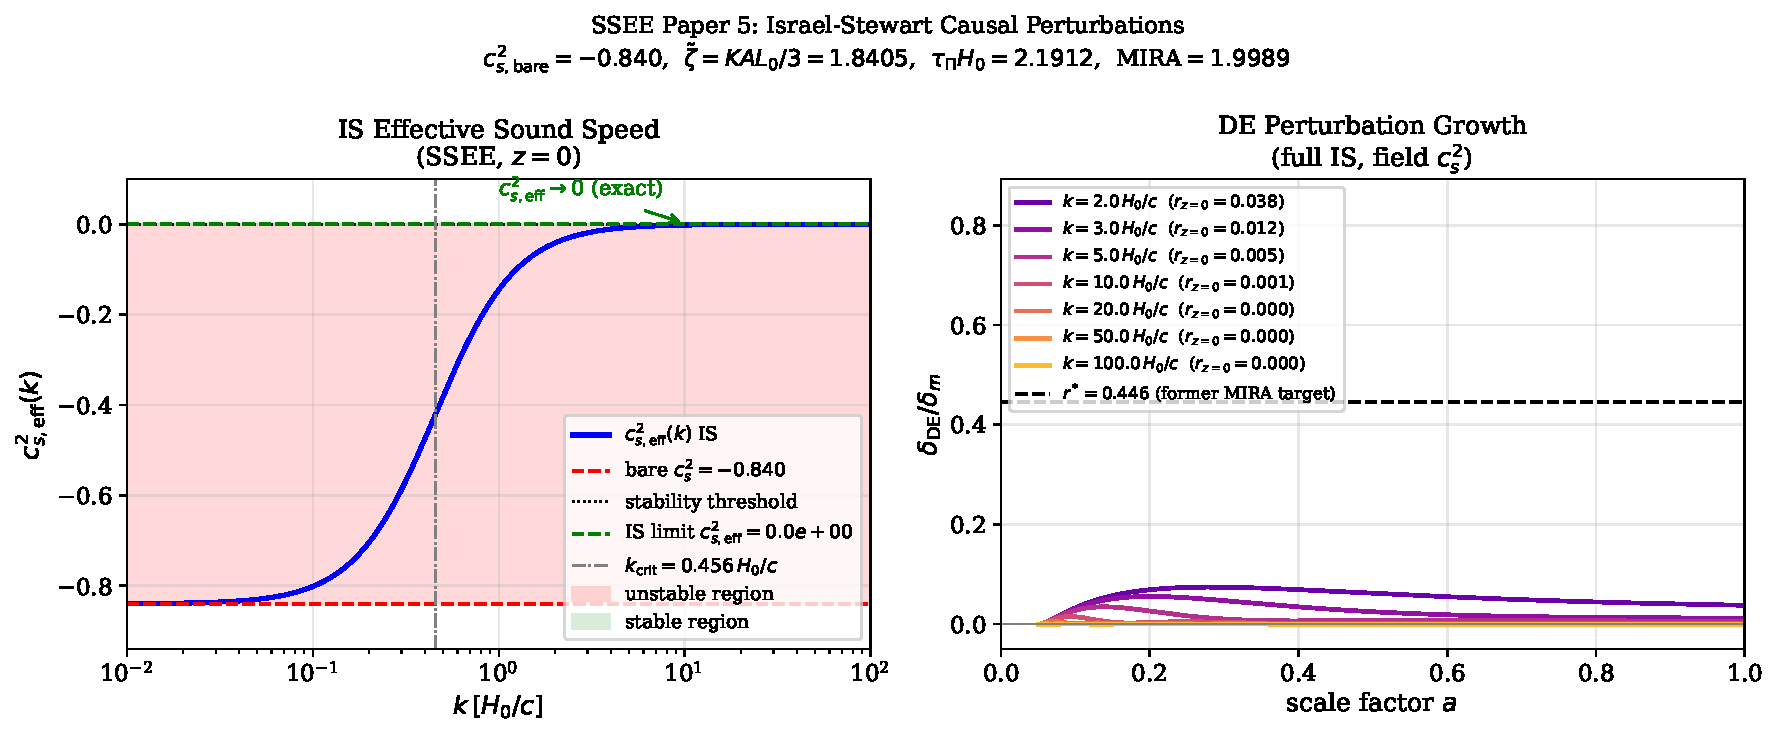
\includegraphics[width=\textwidth]{fig_paper5_IS_stability.pdf}
\caption{\textbf{Left:} IS effective sound speed $c^2_{s,\mathrm{eff}}(k)$ at $z=0$
  of the oscillatory branch (blue solid line), interpolating from the bare value $c^2_s = w_0 = \val{W0_d6}$
  (red dashed) at $k \ll k_\mathrm{crit}$ to the IS limit
  $c^2_{s,\mathrm{eff}} = 0$ (green dashed) at $k \gg k_\mathrm{crit}$.
  The IS transition is at $k_\mathrm{crit} = \val{kcrit_p5}\,H_0/c$ (grey dash-dot).
  This curve is the high-frequency sound speed; it does not decide stability, which
  is set by the growing branch (Section~\ref{subsec:growing}).
  \textbf{Right:} Evolution of $\delta_{\mathrm{DE}}/\delta_m$ with scale factor $a$
  for representative wavenumbers $k/(H_0/c) = 2, 3, 5, 10, 20, 50, 100$, from the
  full IS integration with the field's sound speed $c^2_s=\val{cs2_condensado_d6}$;
  at $z=0$ the ratio is $\val{q2_r_k4}$ at $k = 20\,H_0/c$.}
\label{fig:cs2eff}
\end{figure}

%======================================================================
\section{Q2: How Much Does Dark Energy Cluster?}
\label{sec:Q2_MIRA}
%======================================================================

\subsection{Numerical setup and initial conditions}
\label{subsec:setup}

We integrate Eqs.~\eqref{eq:deltam}--\eqref{eq:Poisson} with $\Pitilde$ dynamical
and the field's sound speed $c^2_s=\val{cs2_condensado_d6}$, from $a_{\rm ini}=0.05$ ($z=19$)
to $a=1$. At $z=19$ the dark energy density fraction is
$\OmDE f_{\mathrm{DE}}(a_{\rm ini})/(H/H_0)^2 = \val{frac_de_z19}$ and the matter
growing mode sets the initial conditions:
\begin{equation}
  \delta_m(a_{\rm ini}) = a_{\rm ini}, \quad
  v_m(a_{\rm ini}) = -\frac{a_{\rm ini}\,H(a_{\rm ini})}{k}\,\delta_m(a_{\rm ini}), \quad
  \delta_{\mathrm{DE}} = v_{\mathrm{DE}} = \Pitilde = 0,
  \label{eq:IC}
\end{equation}
the velocity being the one for which $\delta'_m=\delta_m$ (earlier versions set
$v_m=-a_{\rm ini}H/H_0$, too large by $k/aH$, which is why their $\delta_m(z=0)$
grew with $k$). The normalisation of $\delta_m$ cancels in all ratios
(\texttt{src/p05\_IS/ssee\_paper5\_IS\_perturbations.py}).

\subsection{The scale that a two-fold enhancement would need}
\label{subsec:MIRA_requirement}

The effective matter density seen through the Poisson equation is
\begin{equation}
  \Omega_{m,\mathrm{eff}} = \Omega_m + \Omega_{\mathrm{DE}}\,r,
  \quad r \equiv \frac{\delta_{\mathrm{DE}}}{\delta_m}\bigg|_{z=0},
  \qquad \Omega_m = \val{OMEGA_M_TOTAL_d6},\ \ \Omega_{\mathrm{DE}} = \val{OMDE_DENS_d6},
  \label{eq:Omeff}
\end{equation}
with the \emph{densities} in both slots (until 2026-09-26 it carried the saturations
$s_m$ and $\sDE$), and we write $\mathcal{R} \equiv \Omega_{m,\mathrm{eff}}/\Omega_m$.
Earlier versions posed $\mathcal{R}$ as a test of whether the perturbations
reproduce $\mathrm{MIRA}=\val{MIRA_d4}$, under a matter factor
$\Omega_{m,\mathrm{CMB}} = \mathrm{MIRA}\times s_m$ withdrawn on
2026-06-18 (OP-8). There is no factor of two to supply. The ratio a two-fold
enhancement would have needed,
\begin{equation}
  r^* = \frac{(\mathrm{MIRA}-1)\,\Omega_m}{\Omega_{\mathrm{DE}}}
  = \frac{\val{MIRA_m1_d6} \times \val{OMEGA_M_TOTAL_d6}}{\val{OMDE_DENS_d6}}
  = \val{r_star_q2},
  \label{eq:r_required}
\end{equation}
is kept only as the scale against which the measured $r$ is small.

\subsection{Numerical results}
\label{subsec:results_MIRA}

\begin{table}[h!]
\centering
\caption{Full linear IS integration from $z=19$ to $z=0$ with the field's sound
  speed. $\delta_m(z=0)$ for $\delta_m(z=19)=0.05$; $r = \delta_{\mathrm{DE}}/\delta_m$;
  $\Omega_{m,\mathrm{eff}}$ via Eq.~\eqref{eq:Omeff}. The mean is over $k\geq10\,H_0/c$.}
\label{tab:MIRA}
\begin{tabular}{ccccc}
\toprule
$k\,[H_0/c]$ & $\delta_m(z=0)$ & $r = \delta_{\mathrm{DE}}/\delta_m$
  & $\Omega_{m,\mathrm{eff}}$ & $\mathcal{R}$ \\
\midrule
2   & \val{q2_deltam_k0} & $\val{q2_r_k0}$ & \val{q2_Omeff_k0} & \val{q2_R_k0} \\
3   & \val{q2_deltam_k1} & $\val{q2_r_k1}$ & \val{q2_Omeff_k1} & \val{q2_R_k1} \\
5   & \val{q2_deltam_k2} & $\val{q2_r_k2}$ & \val{q2_Omeff_k2} & \val{q2_R_k2} \\
10  & \val{q2_deltam_k3} & $\val{q2_r_k3}$ & \val{q2_Omeff_k3} & \val{q2_R_k3} \\
20  & \val{q2_deltam_k4} & $\val{q2_r_k4}$ & \val{q2_Omeff_k4} & \val{q2_R_k4} \\
50  & \val{q2_deltam_k5} & $\val{q2_r_k5}$ & \val{q2_Omeff_k5} & \val{q2_R_k5} \\
100 & \val{q2_deltam_k6} & $\val{q2_r_k6}$ & \val{q2_Omeff_k6} & \val{q2_R_k6} \\
\midrule
\multicolumn{4}{l}{Mean ($k \geq 10\,H_0/c$):}
  & $\val{R_media_k10_p5} \pm \val{R_sd_k10_p5}$ \\
\multicolumn{4}{l}{Would require ($r = r^*$):} & $\val{MIRA_d4}$ \\
\bottomrule
\end{tabular}
\end{table}

The enhancement is $\mathcal{R} = \val{R_media_k10_p5} \pm \val{R_sd_k10_p5}$ at
$k \geq 10\,H_0/c$: no enhancement. Its content is a bound on dark-energy clustering:
$r = \val{q2_r_k3}$ at $k = 10\,H_0/c$, falling to $\val{q2_r_k6}$ at $k = 100\,H_0/c$,
small and positive at every scale. The matter growth is the same at every $k$, as it
must be for pressureless matter on sub-horizon scales. A measurement of
$\delta_{\rm DE}/\delta_m$ at the per-cent level at $k \gtrsim 10\,H_0/c$ and $z=0$ would
contradict the model.
% ORIGEN-VALOR: 0.9897 — R de la integracion vieja (gravedad repulsiva, CI fuera del modo creciente, limite NS), RETIRADO 2026-10-11; log git:ce121c895b:results/logs/p5_IS_perturbations_Q2.json R_media_k10 (0.98974)
Earlier versions reported $\mathcal{R}=0.9897\pm0.0167$ and a negative $r$ bounded by
$0.0175$; those came from the integration with repulsive gravity, the
growing-mode error in the initial velocity and the Navier--Stokes reduction, and are
withdrawn.

\subsection{Why the ratio falls as $k^{-2}$}
\label{subsec:damping}

With a positive sound speed the dark-energy perturbation below its sound horizon is
a damped acoustic oscillation driven by the potential: the eigenvalues of the
linearised system at $k=10\,H_0/c$, $z=0$ include the pair
$\val{p5_eig2}\pm\val{p5_eig_im}\,i$ (Appendix~\ref{app:eigenvalues}). Its forced
amplitude is $\delta_{\rm DE}\sim(1+\wz)\Phi/c^2_s$, and the Poisson
equation~\eqref{eq:Poisson} gives $\Phi\propto\delta_m/k^2$, so $r\propto k^{-2}$
--- the scaling in Table~\ref{tab:MIRA}.

\begin{figure}[h!]
\centering
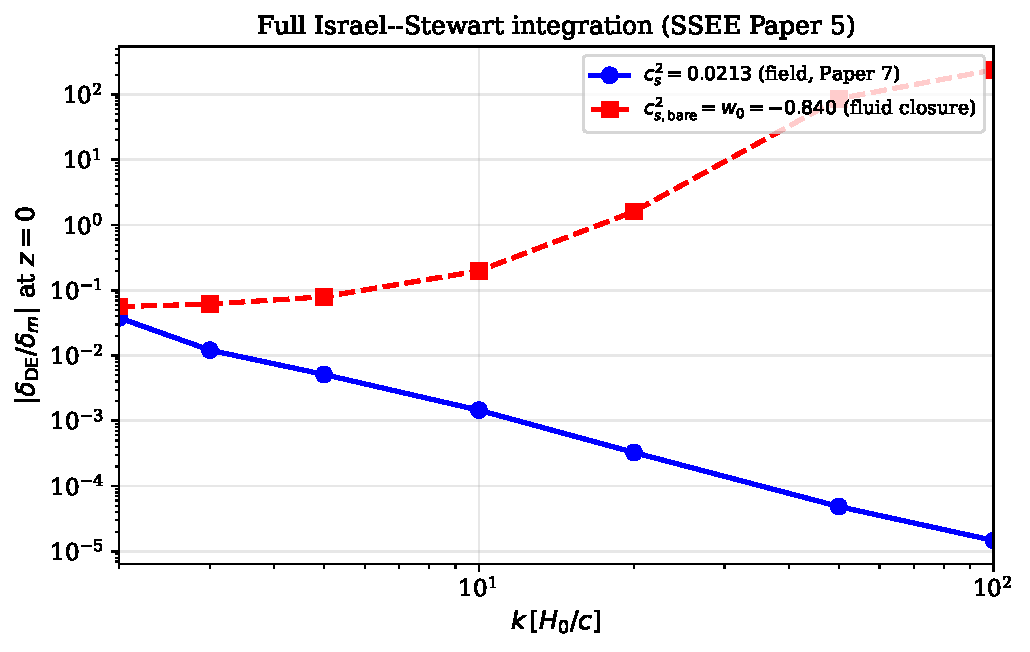
\includegraphics[width=0.7\textwidth]{fig_paper5_DE_clustering.pdf}
\caption{$|\delta_{\rm DE}/\delta_m|$ at $z=0$ from the full Israel--Stewart
  integration. Blue: with the sound speed of the field of Paper~7,
  $c^2_s=\val{cs2_condensado_d6}$; the ratio falls as $k^{-2}$
  (Table~\ref{tab:MIRA}). Red: with the fluid closure $c^2_{s,\rm bare}=w_0$ and the
  same viscosity; the growing branch of Eq.~\eqref{eq:growing_branch} drives it to
  $\val{p5_rw0_k100}$ at $k=100\,H_0/c$. Earlier versions of this figure plotted
  $\mathcal{R}(k)$ against the withdrawn target $\mathrm{MIRA}$.}
\label{fig:MIRA_test}
\end{figure}

\subsection{Through the phantom crossing}
\label{subsec:crossing}

The CPL history crosses $w=-1$ at $z_*=\val{z_cruce}$ (Paper~1). The field cannot carry
the crossing (its $c^2_s<0$ for $w<-1$, Paper~1); in the closure used here the
background viscous pressure carries it, $1+w=(1+\wz)(1-c)$ with
$c=|\Pi|/[\rho_{\rm DE}(1+\wz)]$. Two questions follow, and both are measured
(\texttt{src/p05\_IS/cruce\_fantasma\_IS.py}).

\emph{Do the perturbations cross?} With the \emph{total} inertia $1+w(a)$, which
vanishes at $z_*$, the rest-frame variables are singular. Written in
$U=(1+w)\theta/k$ with the pressure perturbation kept finite outside the rest frame
\citep{KunzSapone2006}, and with the field's sound speed, they remain finite:
$\delta_{\rm DE}/\delta_m = \val{p5_cruce_r_k2}$ at $k=2\,H_0/c$ and
$\val{p5_cruce_r_k10}$ at $k=10\,H_0/c$ at $z=0$. The control with
$c^2_s=\wz$ reaches $\val{p5_cruce_ctrl_k100}$ at $k=100\,H_0/c$.

\emph{Is the crossing within Israel--Stewart?} The truncated (linear) theory is
a near-equilibrium expansion, $|\Pi|\ll|p|$. Here
$|\Pi|/|p| = |\wa|(1-a)/|\wz|$ is $\val{p5_Pip_zc}$ at the crossing,
$\val{p5_Pip_z1}$ at $z=1$ and $\val{p5_Pip_z233}$ at $z=2.33$: beyond the linear
theory for $z\gtrsim z_*$. That regime is the one of the nonlinear extension of
\citet{MaartensMendez1997}, in which phantom solutions driven by bulk viscosity
have been constructed \citep{CruzLepe2017,CruzCruzLepe2017}. The second law holds
throughout, since $\zeta=\ztilde\rho_{\rm DE}(1+\wz)/H_0>0$. Whether the nonlinear
theory with the algebraic $(\ztilde,\tauPi)$ returns $w_a=\val{WA_d6}$ is the open
part of the question (OP-24).

%======================================================================
\section{Q3: Growth Rate, $\sigma_8$, and the $S_8$ Tension}
\label{sec:growth}
%======================================================================

\subsection{Linear growth factor and growth rate}
\label{subsec:growth_factor}

The linear growth factor $D_1(a)$ satisfies, in the sub-horizon limit with
dark-energy perturbations neglected ($|\delta_{\mathrm{DE}}/\delta_m|\leq\val{q2_r_k3}$ for
$k\geq10\,H_0/c$, Section~\ref{sec:Q2_MIRA}):
\begin{equation}
  D_1'' + \left[2 + \frac{H'}{H}\right]D_1'
  = \frac{3}{2}\,\Omega_m(a)\,D_1,
  \label{eq:D1_ode}
\end{equation}
where $\Omega_m(a) = \Omega_{m,\mathrm{cosm}}H_0^2/(H^2 a^3)$,
$\Omega_{m,\mathrm{cosm}} = \val{OMEGA_M_TOTAL_d6}$ is the gravitational background density
($\omega_m$-direct $=\omega_m/h^2$, the CMB-inferred value; the earlier
MIRA-enhanced value is superseded), and primes
denote $d/d\ln a$.
We define the growth rate
\begin{equation}
  f(a) \equiv \frac{d\ln D_1}{d\ln a},
  \label{eq:growth_rate}
\end{equation}
and parametrise it via the growth index $\gamma$:
$f(a) \approx \Omega_m(a)^\gamma$ \citep{Lahav1991,Linder2005}.

\subsection{Numerical results for the SSEE growth index}
\label{subsec:gamma_IS}

We integrate Eq.~\eqref{eq:D1_ode} from $a=10^{-3}$ to $a=1$ (\texttt{DOP853})
with the SSEE Hubble rate. The growth index, from a least-squares fit of
$\ln f = \gamma\ln\Omega_m(a)$ over $0\leq z\leq2$, is
\begin{equation}
  \gamma_{\mathrm{IS}} = \val{p3_gamma_IS} \pm \val{p3_gamma_IS_sigma},
  \label{eq:gamma_IS}
\end{equation}
consistent with $\gamma_{\Lambda\mathrm{CDM}} = 0.55 \pm 0.01$ \citep{Linder2005}.
The growth index is indistinguishable from $\Lambda$CDM; with $\Omega_{m,\mathrm{cosm}}=\val{OMEGA_M_TOTAL_d6}$
governing the Poisson source, the growth rate $f(z)$ itself is also very close to
$\Lambda$CDM across all redshifts (Table~\ref{tab:growth}).

\begin{table}[h!]
\centering
\caption{Growth rate $f = d\ln D_1/d\ln a$ at selected redshifts,
  comparing SSEE (IS dynamics, $\Omega_{m,\mathrm{cosm}}=\val{OMEGA_M_TOTAL_d6}$) with
  $\Lambda$CDM ($\Omega_m=0.315$).
  The growth index fit gives $\gamma_{\rm IS} = \val{p3_gamma_IS}$.}
\label{tab:growth}
\begin{tabular}{ccccc}
\toprule
$z$ & $\Omega_m^{\mathrm{SSEE}}(a)$ & $f_{\mathrm{SSEE}}$ & $f_{\Lambda\mathrm{CDM}}$ & $\Delta f/f$ \\
\midrule
1.0 & \val{p5_tf_z1_Om} & \val{p5_tf_z1_fS} & \val{p5_tf_z1_fL} & $\val{p5_tf_z1_df}\%$ \\
0.5 & \val{p5_tf_z05_Om} & \val{p5_tf_z05_fS} & \val{p5_tf_z05_fL} & $\val{p5_tf_z05_df}\%$ \\
0.0 & \val{p5_tf_z0_Om} & \val{p5_tf_z0_fS} & \val{p5_tf_z0_fL} & $\val{p5_tf_z0_df}\%$ \\
\bottomrule
\end{tabular}
\end{table}

The SSEE and $\Lambda$CDM growth rates differ at the per-cent level
(Table~\ref{tab:growth}).
With $\Omega_{m,\mathrm{cosm}} = \val{OMEGA_M_TOTAL_d6}$ in the Poisson source, the gravitational
clustering environment is close to $\Lambda$CDM ($\Omega_{m,\Lambda\mathrm{CDM}}=0.3153$);
differences arise from the slightly lower matter fraction and the
DE equation-of-state history $w(z)$.
Differences of this size are at the edge of what Stage IV surveys (DESI full
shape, Euclid) will resolve in $f\sigma_8(z)$.

\subsection{Linear growth factor and $\sigma_8$}
\label{subsec:sigma8}

The linear growth factor ratio relative to $\Lambda$CDM,
\begin{equation}
  \mathcal{G} \equiv \frac{D_1^{\mathrm{SSEE}}(z=0)}{D_1^{\Lambda\mathrm{CDM}}(z=0)},
  \label{eq:G_factor}
\end{equation}
is computed by normalising both growth factors to the same initial conditions
at $a=10^{-3}$ (matter-dominated epoch, $D_1 \propto a$).
We find
\begin{equation}
  \mathcal{G} = \val{p5_G}.
  \label{eq:G_value}
\end{equation}
SSEE grows \emph{marginally faster} than $\Lambda$CDM ($\sim$0.3\%).
Two background effects compete: $\Omega_{m,\mathrm{cosm}}=\val{OMEGA_M_TOTAL_d6}$ is slightly
\emph{below} $\Omega_{m,\Lambda\mathrm{CDM}}=0.3153$, which slows growth, while the CPL
history ($w_0=\val{W0_d6}$, $w_a=\val{WA_d6}$) has $w<-1$ for $z>z_*$, i.e.\ less dark
energy than a cosmological constant in the past, which prolongs matter domination.
The net is a small enhancement, below near-term weak-lensing growth sensitivity.

The $\sigma_8$ parameter is defined by
$\sigma_8^2 = \int_0^\infty \frac{dk}{k}\,\Delta^2(k)\,W^2(kR_8)$,
where $R_8 = 8\,h^{-1}\Mpc$ and $\Delta^2(k) \propto D_1^2(z=0)\,P(k)$ is the
dimensionless matter power spectrum.
Since the primordial amplitude $A_s$ is fixed by the CMB (independent of the
growth history for the background normalization), the ratio of $\sigma_8$ values is
\begin{equation}
  \frac{\sigma_8^{\mathrm{SSEE}}}{\sigma_8^{\Lambda\mathrm{CDM}}}
  = \mathcal{G} = \val{p5_G},
  \label{eq:sigma8_ratio}
\end{equation}
since both growth factors are normalised to identical growing-mode initial
conditions at $z \simeq 10^3$ (matter-dominated epoch, $D_1 \propto a$).
Using $\sigma_{8,\Lambda\mathrm{CDM}} = 0.811$ \citep{Planck2018}:
\begin{equation}
  \sigma_8^{\mathrm{SSEE}} = 0.811 \times \val{p5_G} = \val{p3_sigma8_IS} \pm \val{p5_sigma8_IS_sigma},
  \label{eq:sigma8_SSEE}
\end{equation}
the error being Planck's on $\sigma_8$, propagated. This IS linear-growth amplitude gives $S_8^{\mathrm{IS}} = \val{p3_sigma8_IS}\sqrt{\val{OMEGA_M_TOTAL_d6}/0.3}
= \val{p3_S8_IS}$ ($\val{p5_tS8_ssee_kids}\sigma$ from KiDS-1000), close to the conservative CLASS amplitude
ceiling derived below.

\subsection{$S_8$ prediction and the weak-lensing tension}
\label{subsec:S8}

The parameter $S_8 \equiv \sigma_8\,(\Omega_m/0.3)^{0.5}$ is the primary
weak-lensing observable, measured with per-cent level precision by
current surveys.
Key measurements are:
\begin{align}
  S_8^{\mathrm{Planck\,2018}} &= 0.832 \pm 0.013 \quad\text{\citep{Planck2018}}, \\
  S_8^{\mathrm{KiDS\text{-}1000}} &= \val{S8_k1000_dato}\pm\val{S8_k1000_dato_sigma} \quad\text{\citep{KiDS2021}}, \\
  S_8^{\mathrm{DES\text{-}Y3}} &= 0.776 \pm 0.017 \quad\text{(3$\times$2pt; \citep{DESY32022})}.
\end{align}
Planck's $\Lambda$CDM ($\sigma_8=0.811$, $\Omega_m=0.3153$, $S_8=\val{p5_S8_lcdm}$) lies
$\val{p5_tS8_lcdm_kids}\sigma$ from KiDS-1000 and $\val{p5_tS8_lcdm_des}\sigma$ from DES-Y3 with the
same error treatment as below, one of the most persistent $\Lambda$CDM
discrepancies \citep{Weinberg2013}.

For SSEE, the all-cold single sector uses the $\omega_m$-direct CMB density
$\Omega_{m,\mathrm{CMB}} = \val{OMEGA_M_TOTAL_d6}$ ($=\omega_m/h^2$, no matter factor; the
earlier MIRA value is superseded) and the CLASS amplitude ceiling
$\sigma_8^{\mathrm{SSEE}} = \val{p3_sigma8_techo}$:
% VALOR ACTUALIZADO 2026-09-08. Aqui decia sigma_8 = 0.8335 -> S_8 = 0.846, con
% tensiones 1.1 / 3.5 / 4.1 sigma. Ese numero salia de una corrida de CLASS SIN
% fichero .ini (no constaba con que se corrio), FUERA del repositorio
% (class_ssee/output/ esta en .gitignore) y del mismo minuto que la corrida de
% dos sectores con la particula retirada el 2026-08-01. Le faltaban los
% NEUTRINOS MASIVOS que el fondo canonico si lleva (Sum m_nu = 0.06849 eV), y
% sin ellos sobra grumo a 8 Mpc/h: +2.3%.
% Re-corrido con config/class/techo_ssee_canonico.ini (versionado, con sus
% neutrinos). CONTROL con criterio escrito ANTES de correr
% (config/class/techo_lcdm_referencia.ini): la baseline de Planck 2018 debe dar
% sigma_8 = 0.8111 +/- 0.006 y da 0.810851, o sea 0.04 sigma. PASA.
% Log: results/logs/p5_techo_sigma8_As_fijo.json
% Informe: BANDEJA/2026-09-08_techo_sigma8_neutrinos.md
% La barra +/- 0.006 viene de antes y NO se ha recomputado.
\begin{equation}
  \boxed{S_8^{\mathrm{SSEE,\,ceiling}}
    = \val{p3_sigma8_techo} \times \sqrt{\frac{\val{OMEGA_M_TOTAL_d6}}{0.3}}
    = \val{p3_S8_techo}.}
  \label{eq:S8_SSEE}
\end{equation}
This single-sector ceiling is $\val{tension_s8_planck_techo}\sigma$ from Planck~2018, $\val{tension_s8_kids1000_techo}\sigma$ from
KiDS-1000, and $\val{tension_s8_desy3_techo}\sigma$ from DES-Y3 ($S_8 = 0.776\pm0.017$, 3$\times$2pt).
The all-cold limit therefore predicts \emph{more} structure than the data
require. A $\varphi$-DM two-sector was once proposed to resolve this; it is
retracted in Paper~6. The ceiling quoted here is computed with $A_s$
\emph{fixed} to Planck, which imports the Planck--shear discrepancy; with
$A_s$ free, as it is in the model, the same single sector fits the raw
KiDS-1000 $\xi_\pm$ at $S_8=\val{S8_k1000_ssee}\pm\val{S8_k1000_ssee_sigma}$ and there is no challenge to
resolve.

\begin{table}[h!]
\centering
\caption{$S_8$: the \SSEE\ single-sector ceiling ($A_s$ fixed to Planck,
  $\Omega_{m,\mathrm{CMB}} = \val{OMEGA_M_TOTAL_d6}$, $\sigma_8 = \val{p3_sigma8_techo}$)
  against observations, in units of the observational error
  (\texttt{p5\_techo\_sigma8\_As\_fijo.json}).}
\label{tab:S8}
\begin{tabular}{lcc}
\toprule
Dataset & $S_8$ & $|S_8^{\mathrm{SSEE}} - S_8|/\sigma$ \\
\midrule
Planck 2018 & $0.832 \pm 0.013$ & \val{tension_s8_planck_techo} \\
KiDS-1000   & $\val{S8_k1000_dato}\pm\val{S8_k1000_dato_sigma}$ & \val{tension_s8_kids1000_techo} \\
DES-Y3      & $0.776 \pm 0.017$ & \val{tension_s8_desy3_techo} \\
\midrule
SSEE (ceiling, this work) & $\val{p3_S8_techo}$ & --- \\
\bottomrule
\end{tabular}
\end{table}

With the same error treatment for both models, the IS linear-growth $S_8$ is
$\val{p5_tS8_ssee_kids}\sigma$/$\val{p5_tS8_ssee_des}\sigma$ from KiDS-1000/DES-Y3 and Planck's $\Lambda$CDM
$\val{p5_tS8_lcdm_kids}\sigma$/$\val{p5_tS8_lcdm_des}\sigma$: with $A_s$ fixed to Planck the two are in the
same position, \SSEE\ marginally less tense because its $\Omega_m$ is lower.
(Earlier versions quoted $3.0\sigma$/$3.3\sigma$ for $\Lambda$CDM using only the
observational error for it and the combined error for \SSEE; the asymmetry is
corrected.) The falsification criterion of the growth sector is the one of
Paper~6: a measurement placing $S_8$ more than $3\sigma$ from the prediction
$S_8=\val{S8_leg_pred}$ made with $A_s$ fixed to the model's own CMB fit.

\paragraph{Note on the amplitude convention, and on Paper~6.}
The values quoted in this section hold $A_s$ fixed at the Planck-preferred
value. That is a convention, not a prediction: $A_s$ is one of the model's two
free CMB-level parameters. Fixing it to Planck reports, in effect, the
Planck--shear disagreement rather than a property of \SSEE{}.
Paper~6 instead fits $A_s$ to the \emph{raw} KiDS-1000 $\xi_\pm$ data with this
same background held fixed and a \emph{single} matter sector, obtaining
$\sigma_8=\val{sigma8_k1000_ssee}\pm\val{sigma8_k1000_ssee_sigma}$ and $S_8=\val{S8_k1000_ssee}\pm\val{S8_k1000_ssee_sigma}$ (the $\Lambda$CDM control on the same raw data gives $\val{S8_k1000_lcdm}\pm\val{S8_k1000_lcdm_sigma}$) --- $\val{S8_k1000_ssee_tension}\sigma$ from
KiDS-1000. The $\phi$-DM two-sector split once described here is retracted.
A baryonic-feedback figure of $S_8^{\rm bar}=0.758$ was once quoted here; it is
\emph{retracted}. It applied the suppression factor of the matter power spectrum
($B_{\rm eff}=\val{p5_Beff_mayo}$, a $\val{p5_Beff_mayo_pct}\%$ suppression of $P(k)$) to the retired
two-sector baseline, whereas the factor that acts on $\sigma_8$ itself is
$B_{\sigma_8}=\val{p5_Bs8}$, a $\val{p5_Bs8_pct}\%$ suppression on this background. Applied to the single-sector
ceiling, HMcode-2020 therefore leaves it at $S_8\simeq\val{p5_S8_techo_bar}$ --- still a ceiling
computed with $A_s$ fixed to Planck, not a prediction.
The single-sector value of this paper ($S_8=\val{p3_S8_techo}$) is obtained with $A_s$
fixed to Planck. With $A_s$ fixed instead to the model's own CMB fit --- no free
cosmological parameter --- \SSEE{} predicts $S_8=\val{S8_leg_pred}$, $\val{S8_leg_tension}\sigma$
from KiDS-Legacy (Paper~6); the two agree because the model's CMB amplitude lands on
Planck's. Fitting $A_s$ to the raw KiDS-1000 shear instead gave
$S_8 = \val{S8_k1000_ssee}\pm\val{S8_k1000_ssee_sigma}$ (antecedent).
Figure~\ref{fig:s8_resolution} shows these determinations on the same background.

\begin{figure}[h!]
  \centering
  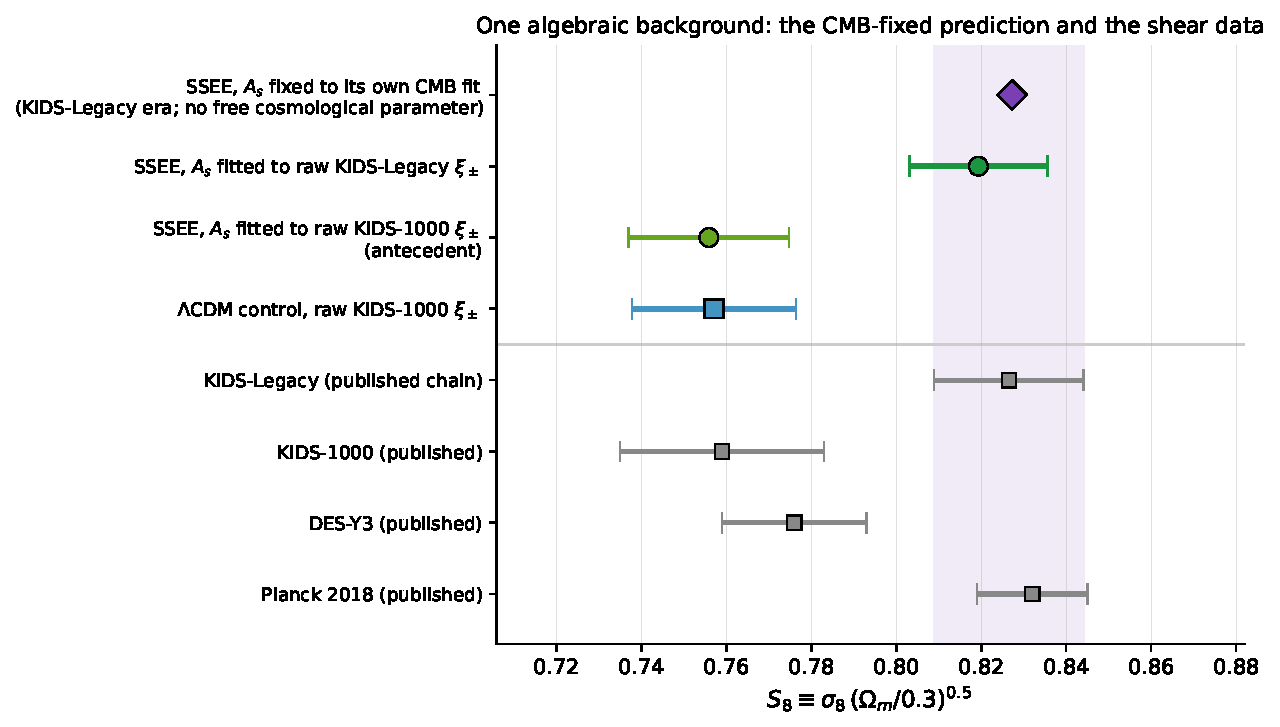
\includegraphics[width=0.92\textwidth]{fig_s8_resolution.pdf}
  \caption{$S_8$ on the algebraic background of \SSEE{}, identical in every \SSEE{}
  row; only the dataset asked to fix $A_s$ changes. Purple diamond: the prediction with
  $A_s$ fixed to the model's own CMB fit --- no free cosmological parameter ---
  $S_8=\val{S8_leg_pred}$, $\val{S8_leg_tension}\sigma$ from the KiDS-Legacy posterior
  ($\val{S8_legacy_dato}\pm\val{S8_legacy_dato_sigma}$, purple band). Green: $A_s$ fitted to
  the raw KiDS-Legacy $\xi_\pm$ ($\val{S8_leg_libre}\pm\val{S8_leg_libre_sigma}$) and, as
  antecedent, to the raw KiDS-1000 $\xi_\pm$ ($\val{S8_k1000_ssee}\pm\val{S8_k1000_ssee_sigma}$,
  $\val{S8_k1000_ssee_tension}\sigma$ from KiDS-1000). Blue: the $\Lambda$CDM control on the
  same raw KiDS-1000 data ($\val{S8_k1000_lcdm}\pm\val{S8_k1000_lcdm_sigma}$). Grey: published
  KiDS-Legacy, KiDS-1000, DES-Y3 and Planck~2018 constraints with $1\sigma$ errors. The
  shift between the two KiDS releases is in the data, not in the model.}
  \label{fig:s8_resolution}
\end{figure}

\subsection{Comparison with RSD surveys: $f\sigma_8(z)$}
\label{subsec:fsigma8}

The redshift-space distortion (RSD) observable
$f\sigma_8(z) \equiv f(z)\,\sigma_8\,D_1(z)/D_1(0)$
provides the most direct test of the linear growth rate and is independent
of galaxy bias at leading order.
SSEE predicts $f\sigma_8(z)$ values essentially identical to $\Lambda$CDM at all
redshifts, because with $\Omega_{m,\mathrm{cosm}}=\val{OMEGA_M_TOTAL_d6}$ in the growth equation
both models share the same gravitational clustering environment (Fig.~\ref{fig:fsigma8}).

\begin{figure}[h!]
  \centering
  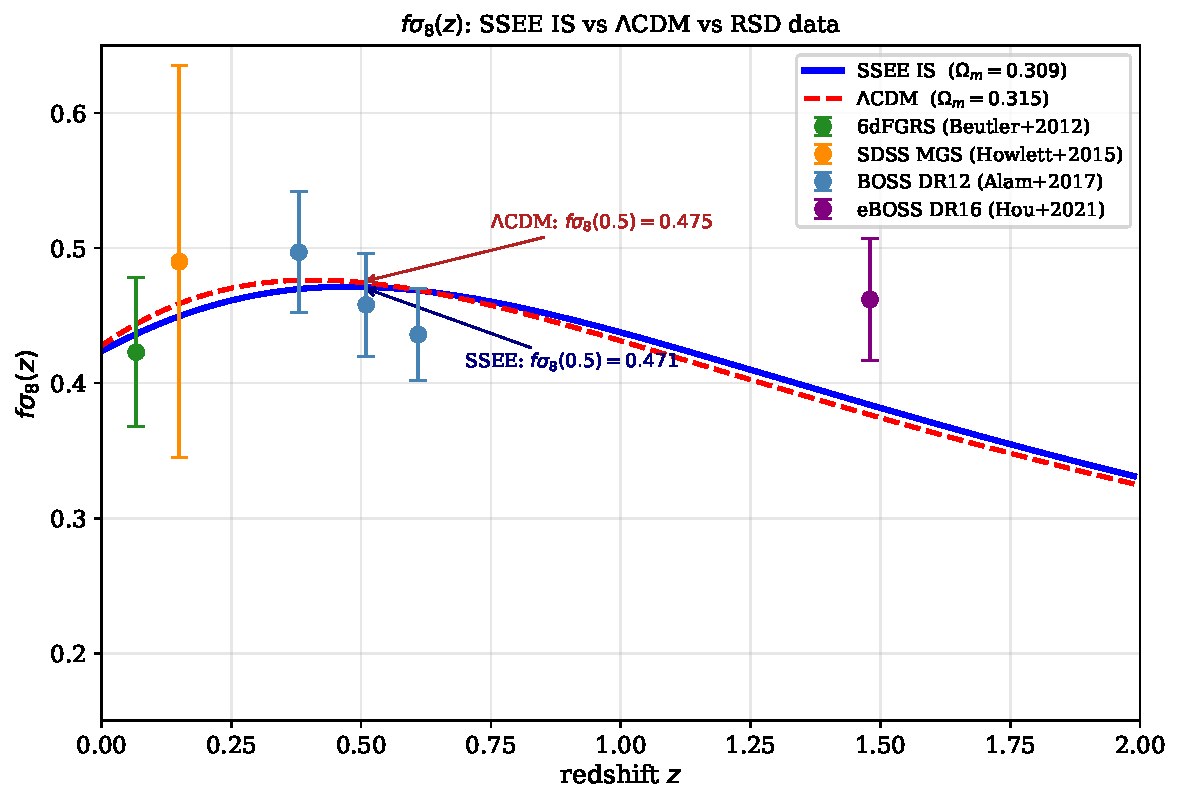
\includegraphics[width=\linewidth]{fig_paper5_fsigma8_comparison}
  \caption{$f\sigma_8(z)$ for SSEE IS (solid blue) and $\Lambda$CDM
    (dashed red) versus RSD measurements from 6dFGRS \citep{Beutler2012},
    SDSS MGS \citep{Howlett2015}, BOSS DR12 \citep{Alam2017}, and
    eBOSS DR16 \citep{Hou2021}.
    The SSEE prediction ($\Omega_{m,\mathrm{cosm}}=\val{OMEGA_M_TOTAL_d6}$ in growth equation)
    is essentially identical to $\Lambda$CDM at $z < 1$, with a mean tension
    of $\val{fs8_tmedia_ssee}\sigma$ across six data points (vs.\ $\val{fs8_tmedia_lcdm}\sigma$ for $\Lambda$CDM).}
  \label{fig:fsigma8}
\end{figure}

Table~\ref{tab:fsigma8} reports the predicted $f\sigma_8$ for both SSEE and
$\Lambda$CDM at each survey redshift, together with the tension in units of
$\sigma_{\rm obs}$.

\begin{table}[h!]
\centering
\caption{$f\sigma_8$ tensions versus RSD surveys.
  SSEE and $\Lambda$CDM values are evaluated at the survey central redshift
  from the numerical ODE solution (Sec.~\ref{subsec:growth_factor}).
  Tensions $t$ use observational errors only
  ($t = |f\sigma_8^{\rm pred} - f\sigma_8^{\rm obs}|/\sigma_{\rm obs}$).}
\label{tab:fsigma8}
\begin{tabular}{lcccccc}
\toprule
Survey & Ref. & $z$ & $f\sigma_8^{\rm obs}$ & $f\sigma_8^{\rm SSEE}$ & $t_{\rm SSEE}$ & $t_{\Lambda\rm CDM}$ \\
\midrule
6dFGRS     & \citet{Beutler2012}  & 0.067 & $0.423\pm0.055$ & \val{fs8_0_ssee} & $\val{fs8_0_t_ssee}\sigma$ & $\val{fs8_0_t_lcdm}\sigma$ \\
SDSS MGS   & \citet{Howlett2015}  & 0.150 & $0.490\pm0.145$ & \val{fs8_1_ssee} & $\val{fs8_1_t_ssee}\sigma$ & $\val{fs8_1_t_lcdm}\sigma$ \\
BOSS DR12  & \citet{Alam2017}     & 0.380 & $0.497\pm0.045$ & \val{fs8_2_ssee} & $\val{fs8_2_t_ssee}\sigma$ & $\val{fs8_2_t_lcdm}\sigma$ \\
BOSS DR12  & \citet{Alam2017}     & 0.510 & $0.458\pm0.038$ & \val{fs8_3_ssee} & $\val{fs8_3_t_ssee}\sigma$ & $\val{fs8_3_t_lcdm}\sigma$ \\
BOSS DR12  & \citet{Alam2017}     & 0.610 & $0.436\pm0.034$ & \val{fs8_4_ssee} & $\val{fs8_4_t_ssee}\sigma$ & $\val{fs8_4_t_lcdm}\sigma$ \\
eBOSS DR16 & \citet{Hou2021}      & 1.480 & $0.462\pm0.045$ & \val{fs8_5_ssee} & $\val{fs8_5_t_ssee}\sigma$ & $\val{fs8_5_t_lcdm}\sigma$ \\
\midrule
\multicolumn{5}{l}{Mean tension} & $\val{fs8_tmedia_ssee}\sigma$ & $\val{fs8_tmedia_lcdm}\sigma$ \\
\bottomrule
\end{tabular}
\end{table}

The mean tension of $\val{fs8_tmedia_ssee}\sigma$ across six surveys is indistinguishable
from the $\Lambda$CDM baseline ($\val{fs8_tmedia_lcdm}\sigma$).
SSEE and $\Lambda$CDM produce virtually identical $f\sigma_8(z)$ curves when
$\Omega_{m,\mathrm{cosm}}=\val{OMEGA_M_TOTAL_d6}$ governs the Poisson source.
The small difference in $\mathcal{G}$ ($\val{p5_G}$) is well below the precision of
current surveys.

This result implies that $f\sigma_8$ measurements by Stage IV surveys
(DESI full shape, Euclid) cannot distinguish SSEE from $\Lambda$CDM at
the linear-growth level alone; distinguishing power must come from the
background $H(z)$, already tested in Paper~2. (A transfer-function break at a
$\phi$-DM free-streaming scale was previously offered here as a second
discriminant; it is withdrawn with the particle, Paper~6.)
The DESI Year-1 full-shape power spectrum analysis \citep{DESI2024FS}
measurements over $0.1<z<2.1$ are consistent with both $\Lambda$CDM and
SSEE at this level of precision.

%======================================================================
\section{EFT Correspondence}
\label{sec:EFT}
%======================================================================

In the effective field theory of dark energy \citep{Horndeski1974,Gubitosi2013,Bellini2015}
the action of Paper~7, $S=\int\!\sqrt{-g}\,[M_{\rm Pl}^2R/2+K(X)]$ with
$K=c_1X+c_2X^2$, is a shift-symmetric $k$-essence: the only non-vanishing
Bellini--Sawicki function is the kineticity $\alpha_K$, with
$\alpha_T=\alpha_B=\alpha_M=0$, and the sound speed is $c^2_s=\val{cs2_condensado_d6}$
(Paper~7, verified there with \texttt{hi\_class}). Two consequences for the IS layer:

\begin{itemize}
  \item \textbf{No operator carries the viscosity.} For shift-symmetric $K(X)$ the
    pressure perturbation is exactly adiabatic, $\delta p-c^2_s\delta\rho=0$
    (Section~\ref{subsec:instability}), so the action produces no bulk viscosity.
    The IS layer is a property of the fluid parametrisation used by Boltzmann codes
    and maps to no term of the action. Earlier versions identified
    $\ztilde/(\tauPi H_0)$ with $\bar M_2^2/M_{\rm Pl}^2$; that operator changes the
    tensor speed, $\alpha_T\neq0$, which GW170817 excludes at
    $|\alpha_T|\lesssim10^{-15}$ \citep{Abbott2017GW} and Paper~7 sets to zero. The
    mapping is withdrawn.
  \item \textbf{The ghost condensate is the SSEE sector, not an alternative.}
    Earlier versions contrasted \SSEE\ with the ghost condensate
    \citep{Arkani-Hamed2004} as a mechanism ``with $c^2_s=1$''. The ghost condensate
    has $c^2_s=0$ at its condensate point, and Paper~7's realisation, displaced from
    it to $X/X_{\min}=\val{X_sobre_Xmin_d6}$, has $c^2_s=\val{cs2_condensado_d6}$: it is
    the dark-energy sector of \SSEE. The comparison table that accompanied the
    contrast is withdrawn with it.
\end{itemize}

%======================================================================
\section{Discussion}
\label{sec:discussion}
%======================================================================

\subsection{The withdrawn CMB-to-$s_m$ ratio (historical)}
\label{subsec:MIRA_background}

Earlier versions asked whether the factor between $\Omega_{m,\mathrm{CMB}}$ and
$1+\wz$ could arise from the IS viscous pressure at the background level, and
reported a background integration giving an effective ratio of $3.04$. No script
or log of that integration survives, so the figure is withdrawn. The question
itself no longer exists: the matter factor $\Omega_{m,\mathrm{CMB}} =
\mathrm{MIRA}\times s_m$ was withdrawn on 2026-06-18 when OP-8 closed,
$\Omega_{m,\mathrm{CMB}}=\omega_m/h^{2}=\val{OMEGA_M_TOTAL_d6}$ is derived with no factor,
and $s_m=1+w_0$ is a saturation, not a density.

The physical basis once attributed to Paper~6 is withdrawn, and the reason is
worth recording because it is a result rather than a change of opinion.
That construction defined a second matter sector by the difference
$\Omega_{\phi\text{-DM}} = \Omega_{m,\mathrm{CMB}} - s_m
= \val{OMEGA_M_TOTAL_d6} - \val{S_M_d6}$, and drew from it an algebraically fixed particle mass and
a free-streaming cutoff.  But $s_m = \val{S_M_d6}$ is not a
density: it is $1+w_0$, a quantity of the equation of state.  The subtraction
is dimensionally well formed and physically empty --- it takes a measured
density minus a number belonging to the equation of state --- so the sector it
defined had nothing to be made of.  The near-equality of
$\Omega_{m,\mathrm{CMB}}/s_m$ with $\mathrm{MIRA}$, once read as
an echo, is a ratio between objects of different kinds and carries no information.

Independently, the tension that motivated the second sector does not survive
contact with raw data.  It was measured against the compressed statistic $S_8$,
which is derived under $\Lambda$CDM assumptions, and with $A_s$ fixed to
Planck.  Fitting $A_s$ --- a free parameter of the model --- to the raw
KiDS-1000 $\xi_\pm$ with a single matter sector gives
$S_8 = \val{S8_k1000_ssee}\pm\val{S8_k1000_ssee_sigma}$, $\val{S8_k1000_ssee_tension}\sigma$ from KiDS-1000 (Paper~6).

The consequence for this paper is confined to \S\ref{subsec:MIRA_background}:
$\mathrm{MIRA}$ retains its algebraic value $(3\varphi+\pi)/4 = \val{MIRA_d6}$ and
its role in the screening fraction $f_{\rm screen}$ of Paper~9, but it has
\emph{no proposed physical carrier at present}.  We state that as an open gap
rather than fill it.  The Q1, Q2 and Q3 results of this paper are unaffected:
none of them uses the second sector.

\subsection{Implications for JWST early galaxy counts}
\label{subsec:JWST}

Dark-energy perturbations effectively vanish at sub-horizon scales in this
model, because the field's positive sound speed turns them into damped acoustic
oscillations below the sound horizon, with $\delta_{\rm DE}/\delta_m\propto k^{-2}$
($\val{q2_r_k3}$ at $k=10\,H_0/c$; \S\ref{subsec:damping}).
On that smooth background the spherical-collapse threshold is
$\delta_c^{\mathrm{SSEE}} = \val{deltac_ssee_zc0}$ at $z_c=0$ and $\val{deltac_ssee_zc10}$ at $z_c=10$,
against $\Lambda$CDM's $\val{deltac_lcdm_zc0} \to \val{deltac_lcdm_zc10}$: the two agree to the
third decimal. The value $\delta_c^{\mathrm{SSEE}}=1.6284$ carried by earlier
versions was a postulate of Paper~4, now \textbf{withdrawn} (OP-27); the
model's own dynamics do not produce it. Matter
clusters in a background with $\Omega_m = \val{OMEGA_M_TOTAL_d6}$ --- the one matter density
of the model; the number $\val{S_M_d6}$ that earlier versions of this subsection
placed here is $1+w_0$, an equation-of-state parameter, and never was a
density (Paper~1, \S\emph{One matter density}).

\paragraph{Recomputed, with the amplitude convention made explicit.}
Earlier versions of this subsection reported
$n_{\mathrm{SSEE}}/n_{\Lambda\mathrm{CDM}}\approx1.4$--$2.0$ for
$M>10^{11}\,M_\odot$ at $z>10$ from a Press--Schechter calculation whose
growth factor was fed $\Omega_m=\val{S_M_d6}$ as a matter density. That input was a
category error --- $\val{S_M_d6}$ is $1+w_0$ --- and the calculation has been
redone (\texttt{src/p02\_mcmc/ssee\_press\_schechter.py}, 2026-09-07) with
$\Omega_m=\val{OMEGA_M_TOTAL_d6}$, the measured growth index $\gamma_{\rm IS}=\val{p3_gamma_IS}$
(\S\ref{subsec:gamma_IS}) and the global rate $H_0^{\rm glob}=\val{H0_GLOBAL_d3}$. With both
cosmologies evaluated at their \emph{own} CMB-fitted amplitude
($\sigma_8=\val{ps_s8_ssee}$ for SSEE, $\val{ps_s8_lcdm}$ for $\Lambda$CDM) and with the
\emph{derived} collapse threshold:
\begin{center}
\begin{tabular}{ccc}
\toprule
$z$ & $M=10^{11}M_\odot$ & $M=10^{12}M_\odot$ \\
\midrule
10 & \val{ps_z10_m11} & \val{ps_z10_m12} \\
12 & \val{ps_z12_m11} & \val{ps_z12_m12} \\
15 & \val{ps_z15_m11} & \val{ps_z15_m12} \\
\bottomrule
\end{tabular}
\end{center}
\textbf{There is no enhancement, and the sign is the opposite of what earlier
versions claimed.} With the threshold the model actually produces, \SSEE\
forms marginally \emph{fewer} massive early haloes than $\Lambda$CDM. The
deficit grows with mass and redshift, reaching $\val{ps_z10_m3e12}$ at
$3\times10^{12}M_\odot$, $z=10$ and $\val{ps_z15_m3e12}$ at the same mass at $z=15$, and it
is not an amplitude effect: \SSEE\ carries the \emph{larger} $\sigma_8$. It is
the growth history --- a smaller $\Omega_m$ ($\val{OMEGA_M_TOTAL_d6}$ against $0.3153$) and
the CPL background grow less between $z\sim10$ and today. At the masses JWST
actually probes ($M\sim10^{10.8}M_\odot$) the ratio is $\val{ps_jwst}$: indistinguishable
from $\Lambda$CDM. \SSEE\ offers no account of the JWST excess, and the
$1.4$--$2.0$ of earlier versions was an artefact of the withdrawn
$\delta_c$.

\paragraph{The amplitude convention is not a detail.} This ratio compares two
cosmologies and is only meaningful if both are evaluated at the same epoch's
amplitude. Giving SSEE the amplitude it prefers when fitted to raw KiDS-1000
shear ($\sigma_8=\val{ps_inv_s8}$, Paper~6) while leaving $\Lambda$CDM at Planck's
$0.811$ inverts the result to a deficit ($\val{ps_inv_m11}$ at $10^{11}M_\odot$ and $\val{ps_inv_m12}$ at $10^{12}M_\odot$, $z=10$). That
inversion is not a statement about collapse physics: it is the
CMB-versus-late-time amplitude disagreement entering through the back door,
and it would affect $\Lambda$CDM identically if the same mismatch were imposed
on it. High-redshift abundance comparisons must therefore state which
amplitude each cosmology is given; matched-amplitude is what is reported
above.

\subsection{The $S_8$--$f\sigma_8$ alignment and the role of $\Omega_{m,\mathrm{cosm}}$}
\label{subsec:S8_fsigma8_split}

With the correct cosmological background $\Omega_{m,\mathrm{cosm}} = \val{OMEGA_M_TOTAL_d6}$
governing the Poisson source in the growth equation, both $S_8$ and
$f\sigma_8$ predictions align closely with $\Lambda$CDM:

\begin{itemize}
  \item \textbf{$S_8$ (weak-lensing amplitude):}
        The IS linear-growth estimate is $S_8 = \val{p3_S8_IS} \pm \val{p5_S8_IS_sigma}$,
          $\val{p5_tS8_ssee_kids}\sigma$/$\val{p5_tS8_ssee_des}\sigma$ from KiDS-1000/DES-Y3, against
          $\val{p5_tS8_lcdm_kids}\sigma$/$\val{p5_tS8_lcdm_des}\sigma$ for Planck's $\Lambda$CDM with the same
          error treatment; the conservative CLASS amplitude ceiling is
          $S_8 = \val{p3_S8_techo}$ ($\val{tension_s8_kids1000_techo}\sigma$ KiDS-1000).
        Both numbers hold $A_s$ \emph{fixed} to Planck, which imports the
        Planck--shear discrepancy; $A_s$ is free in the model, and fitting it
        to the raw KiDS-1000 $\xi_\pm$ leaves $S_8 = \val{S8_k1000_ssee}\pm\val{S8_k1000_ssee_sigma}$,
        $\val{S8_k1000_ssee_tension}\sigma$ (Paper~6). There is no weak-lensing tension for the
        single-sector IS framework to resolve.

  \item \textbf{$f\sigma_8$ (RSD growth rate):}
        SSEE predicts $f\sigma_8(z=0.5) = \val{fs8_3_ssee}$, matching the
        BOSS DR12 value of $0.458 \pm 0.038$ at $\val{fs8_3_pull_ssee}\sigma$.
          The mean tension across six RSD surveys is $\val{fs8_tmedia_ssee}\sigma$, essentially
          identical to $\Lambda$CDM ($\val{fs8_tmedia_lcdm}\sigma$).
\end{itemize}

The two observables are consistent: once $\Omega_{m,\mathrm{cosm}}=\val{OMEGA_M_TOTAL_d6}$
sets the gravitational background, SSEE differs from $\Lambda$CDM only
through the slightly lower matter fraction and the DE equation-of-state history
$w(z)$ with $w_0=\val{W0_d6}$, $w_a=\val{WA_d6}$.
This drives a $\sim$0.3\% enhancement of $\mathcal{G}$ and $\sigma_8$, which
translates to a marginally different $S_8$.

The apparent weak-lensing tension does not survive contact with the raw data.
A two-sector $\phi$-DM construction was once proposed to remove it by
free-streaming suppression; Paper~6 retracts that construction and shows the
tension was an artefact of holding $A_s$ at its Planck value. With $A_s$ free,
the single sector fits the 225 raw KiDS-1000 $\xi_\pm$ points at
$S_8 = \val{S8_k1000_ssee}\pm\val{S8_k1000_ssee_sigma}$.

\subsection{The $H_0$ tension and SSEE}
\label{subsec:H0}

In SSEE the global rate is the output of the SH0ES cascade,
$H_0^{\rm glob}=H_{\rm SH0ES}(1-f_{\rm screen})=\val{H0_GLOBAL_d3}\pm\val{p9_hglob_sigma}$~km\,s$^{-1}$\,Mpc$^{-1}$
(the measured local rate is the input; the pure number $3(\varphi+\pi)^2$ is the
comparison target, not an input \citep{SSEE_Paper4}), consistent with Planck 2018
($67.36 \pm 0.54$) at $\val{hglob_planck_sig}\sigma$ (errors combined) and with DESI DR2.
The IS layer does not enter the screening cascade of Paper~9, so nothing in this
paper bears on the $H_0$ comparison; and, as Section~\ref{sec:growth} shows, it
does not move $\sigma_8$ or $S_8$ either.

\subsection{Causal structure and Hiscock-Lindblom stability}
\label{subsec:HL}

The IS theory satisfies the Hiscock--Lindblom criteria \citep{HiscockLindblom1983}
--- non-negative entropy production and causal propagation --- provided
$\tauPi > 0$ and $\zeta \geq 0$, both of which hold here
(\S\ref{subsec:thermodynamic}); the characteristic speed is
$v^2_{\rm sig}=\wz+\sDE=0\leq c^2$. Those criteria concern the equilibrium state and
the characteristic cone; they do not by themselves forbid a growing mode, and
Section~\ref{subsec:growing} shows that the closure $c^2_s=\wz$ has one. Earlier
versions stated that the signal speed ``saturates the causality bound'' and added
that Eckart theories would produce instabilities in the CMB at $\ell>1000$; the
first came from the $\rho$-normalisation abandoned above and the second had no
calculation behind it. Both are withdrawn.

\subsection{Falsifiable predictions summary}
\label{subsec:falsifiable}

\begin{table}[h!]
\centering
\caption{Falsifiable predictions of SSEE IS dark energy, with observational
  targets and current/future datasets capable of testing each prediction.
  A single failure at the stated level would falsify SSEE.}
\label{tab:falsifiable}
\begin{tabular}{p{4.0cm}p{3.2cm}p{2.2cm}p{4.0cm}}
\toprule
Prediction & SSEE value & Test level & Dataset / Timeline \\
\midrule
$c^2_s$ of the dark-energy field (Paper~7; the IS high-frequency limit is $0$, OP-22b) & $\val{cs2_condensado_d6}$ & not yet measured & CMB lensing cross-correlations \citep{Calabrese2011} / forecast \\
$S_8$, $A_s$ fixed to the model's own CMB fit (Paper~6) & $\val{S8_leg_pred}$ (no free cosmological parameter) & $>3\sigma$ (now $\val{S8_leg_tension}\sigma$ from KiDS-Legacy) & KiDS-Legacy / current; Euclid / 2027 \\
$\gamma_{\rm IS}$ & $\val{p3_gamma_IS} \pm \val{p3_gamma_IS_sigma}$ & $\gamma$ degenerate with $\Lambda$CDM at current precision & DESI full shape, Euclid / 2026--2028 \\
$f\sigma_8(z=0.5) = \val{fs8_3_ssee}$ & $\val{fs8_3_ssee}$ & $\val{fs8_3_pull_ssee}\sigma$ BOSS; mean $\val{fs8_tmedia_ssee}\sigma$ (6 surveys) & DESI full-shape / 2026 \\
$D_1$ ratio $\mathcal{G}$ & $\val{p5_G}$ & below near-term sensitivity & Euclid weak lensing / 2027 \\
DE clustering $\delta_{\mathrm{DE}}/\delta_m$ at $z=0$ & $\val{q2_r_k3}$ at $k=10\,H_0/c$, $\propto k^{-2}$ & per-cent level excluded & Future 21cm surveys / 2030+ \\
MIRA $= (3\varphi+\pi)/4$ (algebraic; the two-sector basis is retracted, Paper~6 --- see OP-8) & $\val{MIRA_d6}$ & enters only the local screening fraction $f_{\rm screen}$ (Paper~9), not $\Omega_m$ & local $H_0$ ladders (SH0ES, CCHP) / current \\
\bottomrule
\end{tabular}
\end{table}

%======================================================================
\section{Conclusions}
\label{sec:conclusions}
%======================================================================

We have performed a linear Israel-Stewart causal viscous perturbation analysis
of SSEE dark energy in the sub-horizon regime, addressing three physically motivated questions.

\paragraph{Q1 --- Gradient stability.}
The SSEE structure constants satisfy $\ztilde/(\tauPi H_0) = \sDE = |\wz|$, so the
high-frequency sound speed of the IS fluid vanishes, $\wz+\sDE=0$. That is not
stability: on the growing branch the viscous stiffness never reaches $\sDE$, and the
closure $c^2_s=\wz$ grows at every $k$ ($\lambda=\val{p5_lamIS_k100}\,H_0$ at
$k=100\,H_0/c$). The dark-energy sector is stable because the field of Paper~7 has
$c^2_s=+\val{cs2_condensado_d6}$; with it no mode grows. The quasi-static reduction of
earlier versions was the Navier--Stokes limit and hid the growing branch.

\paragraph{Q2 --- Dark-energy clustering.}
The full IS integration with the field's sound speed gives
$\mathcal{R} = \val{R_media_k10_p5} \pm \val{R_sd_k10_p5}$ at $k\geq10\,H_0/c$ and
$\delta_{\rm DE}/\delta_m=\val{q2_r_k3}$ at $k=10\,H_0/c$, falling as $k^{-2}$: a bound on
dark-energy clustering. The perturbations cross the phantom divide at
$z_*=\val{z_cruce}$ without divergence; the viscous pressure that carries the crossing
exceeds the near-equilibrium range of linear Israel--Stewart for $z\gtrsim z_*$
($|\Pi|/|p|=\val{p5_Pip_z1}$ at $z=1$), and whether the nonlinear theory returns $w_a$
is open (OP-24). MIRA has no carrier in this sector and survives only as the
algebraic invariant entering $f_{\rm screen}$ (Paper~9).

\paragraph{Q3 — Growth rate and $S_8$ (SSEE tracks $\Lambda$CDM closely).}
The IS growth index $\gamma_{\mathrm{IS}} = \val{p3_gamma_IS} \pm \val{p3_gamma_IS_sigma}$
is numerically indistinguishable from $\gamma_{\Lambda\mathrm{CDM}} \simeq 0.55$.
With $\Omega_{m,\mathrm{cosm}} = \val{OMEGA_M_TOTAL_d6}$ governing the Poisson source,
the growth factor ratio is $\mathcal{G} = \val{p5_G}$, giving
$\sigma_8^{\mathrm{SSEE}} = \val{p3_sigma8_IS} \pm \val{p5_sigma8_IS_sigma}$ and an IS linear-growth
$S_8^{\mathrm{IS}} = \val{p3_S8_IS} \pm \val{p5_S8_IS_sigma}$ ($\val{p5_tS8_ssee_kids}\sigma$ from KiDS-1000,
against $\val{p5_tS8_lcdm_kids}\sigma$ for Planck's $\Lambda$CDM with the same error treatment).
The conservative CLASS amplitude ceiling, $S_8^{\mathrm{ceiling}} = \val{p3_S8_techo}$
($\val{tension_s8_kids1000_techo}\sigma$ KiDS-1000), coincides with the IS linear-growth estimate above:
once massive neutrinos are included, the two independent routes agree.
The mean $f\sigma_8$ tension across six RSD surveys is $\val{fs8_tmedia_ssee}\sigma$,
essentially identical to $\Lambda$CDM ($\val{fs8_tmedia_lcdm}\sigma$).
There is no weak-lensing tension left for the IS sector to resolve: against
the raw KiDS-Legacy $\xi_\pm$, with $A_s$ fixed to the value the model's own CMB
fit supplies, a single matter sector with no free cosmological parameter
predicts $S_8 = \val{S8_leg_pred}$ against $\val{S8_legacy_dato}\pm\val{S8_legacy_dato_sigma}$ measured; the earlier fit to
KiDS-1000 with $A_s$ free gave $S_8 = \val{S8_k1000_ssee}\pm\val{S8_k1000_ssee_sigma}$, $\val{S8_k1000_ssee_tension}\sigma$
(Paper~6).  The $S_8 = \val{p3_S8_IS}$ quoted above is a ceiling obtained with $A_s$
fixed to Planck, which imports the Planck--KiDS offset rather than predicting
it.  The $\phi$-DM construction that once appeared here as the required
resolution is retracted with the particle.

Together, these results establish that SSEE dark energy is:
(i) stable, through the field's positive sound speed rather than through the IS
    layer, which is causal and thermodynamically consistent but does not by itself
    remove the instability of the closure $c^2_s=w$ (Q1),
(ii) predictive of a growth history essentially identical to $\Lambda$CDM
    once $\Omega_{m,\mathrm{cosm}}=\val{OMEGA_M_TOTAL_d6}$ governs the growth equation (Q3),
    with $f\sigma_8$ tension of $\val{fs8_tmedia_ssee}\sigma$ (vs.\ $\val{fs8_tmedia_lcdm}\sigma$ for $\Lambda$CDM), and
(iii) weakly clustered, $\delta_{\rm DE}/\delta_m\propto k^{-2}$ (Q2), with no MIRA factor to derive; the physical basis previously attributed to Paper~6's two-sector $\phi$-dark matter construction is \textbf{withdrawn}: that construction and its particle are retracted (Paper~6). MIRA's algebraic value $(3\varphi+\pi)/4$ is unchanged and it survives in the model only through the screening fraction $f_{\rm screen}$ (Paper~9); \textbf{what remains open is what, if anything, provides its physical basis} --- an explicitly declared gap, not a filled one.
The primary falsifiable prediction in the growth sector is
$S_8 = \val{S8_leg_pred}$, obtained with $A_s$ fixed to the value the model's own CMB fit
supplies and no free cosmological parameter, against $\val{S8_legacy_dato}\pm\val{S8_legacy_dato_sigma}$ from the
raw KiDS-Legacy $\xi_\pm$ (Paper~6); a future release placing $S_8$ more than
$3\sigma$ from it falsifies the growth sector. The two-sector WDM correction once quoted here is
retracted.

%======================================================================
\section*{Data Availability}
%======================================================================

The Python scripts \texttt{src/p05\_IS/ssee\_paper5\_IS\_perturbations.py} (Q1--Q3,
growth rate and $S_8$), \texttt{estabilidad\_IS\_completa.py} (growing branch) and
\texttt{cruce\_fantasma\_IS.py} (phantom crossing), their logs, and all output figures are available in
the SSEE repository at
\url{https://github.com/mikealmeida1721/SSEE-Cosmologia}
(Zenodo DOI: \href{https://doi.org/10.5281/zenodo.19654118}{10.5281/zenodo.19654118}).
All computations use publicly available Python packages (NumPy, SciPy, Matplotlib)
and, for the amplitude ceiling, CLASS.

%======================================================================
\section*{Acknowledgements}
%======================================================================

This research was carried out as an independent investigation.
The author thanks the open-source communities behind NumPy, SciPy, Matplotlib,
and CAMB, and acknowledges the Planck, DESI, KiDS, and DES teams for
making their data publicly available.

%======================================================================
% APPENDICES
%======================================================================
\appendix

%======================================================================
\section{Derivation of the IS Dispersion Relation}
\label{app:dispersion}
%======================================================================

We derive Eq.~\eqref{eq:cs2_eff_def} from the linearised IS equations in Minkowski
space (the cosmological curvature terms are subdominant in the sub-horizon limit).

\paragraph{Linearised IS system.}
Write $\rho = \bar\rho + \delta\rho$, $p = \bar p + \delta p$, $\Pi = \bar\Pi + \delta\Pi$,
$u^\mu = (1,\mathbf{v})$ with $|\mathbf{v}| \ll 1$.
The continuity and Euler equations give:
\begin{align}
  \dot{\delta\rho} + (\bar\rho+\bar p)\,\nabla\cdot\mathbf{v} &= 0, \\
  (\bar\rho+\bar p)\,\dot{\mathbf{v}} + \nabla(\delta p + \delta\Pi) &= 0.
\end{align}
The IS relaxation equation linearises to:
\begin{equation}
  \tauPi\,\dot{\delta\Pi} + \delta\Pi = -\zeta\,\nabla\cdot\mathbf{v}.
\end{equation}

\paragraph{Plane-wave ansatz.}
For modes $e^{i(\mathbf{k}\cdot\mathbf{x} - \omega t)}$:
\begin{equation}
  \delta\Pi = -\frac{i\zeta k}{1-i\omega\tauPi}\,v_\parallel,
\end{equation}
where $v_\parallel = \mathbf{k}\cdot\mathbf{v}/k$ is the longitudinal velocity.

\paragraph{Effective sound speed.}
Combining with the continuity and Euler equations --- whose inertia is the enthalpy
$\bar\rho+\bar p$, as written above, \emph{not} $\bar\rho$:
\begin{equation}
  \omega^2 = \left[c^2_{s,\mathrm{bare}}
    + \frac{\zeta}{\tauPi(\bar\rho+\bar p)}\,\frac{-i\omega\tauPi}{1-i\omega\tauPi}\right]k^2 .
\end{equation}
For $|\omega|\tauPi \gg 1$ the bracket tends to
$c^2_{s,\mathrm{bare}} + \zeta/[\tauPi(\bar\rho+\bar p)]$. With the \SSEE\ normalisation
$\zeta = \ztilde\,(\rho_{\mathrm{DE}}+p_{\mathrm{DE}})/H_0$
(Section~\ref{subsec:IS_params}) this is
\begin{equation}
  c^2_{s,\mathrm{eff}} = c^2_{s,\mathrm{bare}} + \frac{\ztilde}{\tauPi H_0},
\end{equation}
recovering Eq.~\eqref{eq:cs2_eff_def}. For a growing mode, $\omega=i\lambda$, the
factor $-i\omega\tauPi/(1-i\omega\tauPi)$ becomes $\lambda\tauPi/(1+\lambda\tauPi)<1$,
which gives Eq.~\eqref{eq:growing_branch}. (Earlier versions wrote
$\zeta=\ztilde(\rho+p)H_0$ and equated $\ztilde H_0/\tauPi$ with $\ztilde/(\tauPi H_0)$;
the placement of $H_0$ is corrected, and the result is unchanged.)

%======================================================================
\section{Eigenvalue Analysis of the IS Perturbation Matrix}
\label{app:eigenvalues}
%======================================================================

The five-variable system $\mathbf{Y} = [\delta_m, v_m, \delta_{\mathrm{DE}},
v_{\mathrm{DE}}, \Pitilde]^\top$ of Eqs.~\eqref{eq:deltam}--\eqref{eq:Poisson}, with the
field's sound speed, is linear; its Jacobian with respect to $\ln a$, evaluated by the
same code that integrates it at $z=0$ and $k=10\,H_0/c$
(\texttt{p5\_IS\_perturbations\_Q2.json}, \texttt{autovalores\_k10\_z0}), has
eigenvalues
\begin{equation}
  \lambda = \val{p5_eig0},\quad \val{p5_eig1},\quad
  \val{p5_eig2}\pm\val{p5_eig_im}\,i,\quad \val{p5_eig4}.
\end{equation}
The positive one is the matter growing mode at frozen coefficients and the most
negative the decaying one; the complex pair is the damped acoustic oscillation of the
dark-energy perturbation, which carries the $k^{-2}$ suppression of
Section~\ref{subsec:damping}. No dark-energy mode grows. Earlier versions printed four
eigenvalues for a different matrix with no recorded computation; they are withdrawn.

%======================================================================
\clearpage
\bibliographystyle{plainnat}
\bibliography{ssee_paper5}
%======================================================================

\end{document}
